% !TEX TS-program = xelatex
% !TEX encoding = UTF-8

% This is a simple template for a XeLaTeX document using the "article" class,
% with the fontspec package to easily select fonts.

\documentclass[oneside,10pt]{book} % use larger type; default would be 10pt

% other LaTeX packages.....

%-------------------------------------------------
% Geometry (et sidenotes) : format tufte light
%-------------------------------------------------

\usepackage{sidenotes}

%\usepackage{mwe}

%\usepackage[showframe]{geometry}
\usepackage{geometry}

% option classique
\geometry{letterpaper, left=2cm, right=3in, top=50pt,bottom=50pt, marginparsep=20pt, marginparwidth=2in,  footskip=40pt}

% Option pour faire un document A5
%\geometry{paperwidth=6in, paperheight=9in, left=2cm, right=2in, top=50pt,bottom=50pt, marginparsep=20pt, marginparwidth=1.5in,  footskip=40pt}
 
\renewcommand{\baselinestretch}{1.1} 
\usepackage{placeins} % floatbarrier
\usepackage{fullwidth}
 
\makeatletter
%\renewcommand{\@sidenotes@adjust}{%
% \checkoddpage%
% \ifoddpage%
% %
% \else%
% %\hspace{\@sidenotes@extrawidth}%    %% this was originally there
% \fi}
%%
%% or
%%
\let\@sidenotes@adjust\relax
\makeatother

\setlength\parindent{0pt}
%\usepackage{marginnote}
%\renewcommand*{\raggedleftmarginnote}{}
%\renewcommand*{\raggedrightmarginnote}{}

% Margin Caption (done with sidenotes package)
% UTILISER \sidecaption pour une caption
%\usepackage[margincaption,rightcaption,ragged,wide]{sidecap}
%\usepackage[margincaption,outercaption]{sidecap}
%\sidecaptionvpos{figure}{t} 
%\sidecaptionvpos{table}{t}
% format des captions des figures
%\captionsetup[SCfigure]{format=plain, ...}
%\captionsetup[SCtable]{format=plain, ...}
%-------------------------------------------------
% cadre
%-------------------------------------------------

\usepackage{tikz}
\usepackage[framemethod=TikZ]{mdframed}
\usetikzlibrary{positioning}  
\usepackage{placeins} % FLoatbarrier to force float

\usepackage{xcolor}
%\hypersetup{colorlinks}% uncomment this line if you prefer colored hyperlinks (e.g., for onscreen viewing)
\usepackage{units}
% Typesets the font size, leading, and measure in the form of 10/12x26 pc.


\newcommand{\measure}[3]{#1/#2$\times$\unit[#3]{pc}}
\newcommand{\coefGraph}{1} % Taille du graphe dans les marges; sert uniquement pour Epub, sinon = 1 x textwidth
%\usepackage{multicol} %multicolum for Definition
\newcommand{\largecoefGraph}{1.2} % Taille du graphe dans les marges en proportion de textwidth; sert uniquement pour Epub, sinon = textwidth; remplacer \textwidth par \coefGraph\textwidth
%\usepackage[table]{xcolor}
%\usepackage[xcdraw]{xcolor}
%\usepackage[dvipsnames]{xcolor}
%\usepackage{amsmath,amssymb,amsthm}
%\usepackage{mathtools}
%\usepackage{mathspec}
%\usepackage{xltxtra,xunicode}
\newcommand{\myinnertopmargin}{0pt} % marge qui sert pour les définitions et proprietés




%-------------------------------------------------
% url
%-------------------------------------------------

\usepackage{blindtext}
\usepackage{hyperref}
\usepackage{url}


%-------------------------------------------------
% tableau
%-------------------------------------------------

% pour mettre des tableaux au bon endroit avec l'option H
%\usepackage{float}
% grands tableaux... pratiques
\usepackage{longtable}
 % pour faire des beaux tableaux
\usepackage{booktabs}

 
%-------------------------------------------------
% caractère
%-------------------------------------------------




\usepackage[sc]{mathpazo}
\linespread{1.05}         % Palladio needs more leading (space between lines)

\usepackage{fontspec} % Font selection for XeLaTeX; see fontspec.pdf for documentation
\defaultfontfeatures{Mapping=tex-text} % to support TeX conventions like ``---''


%\setmainfont{Charis SIL} % set the main body font (\textrm), assumes Charis SIL is installed
%\setsansfont{Deja Vu Sans}
%\setmonofont{Deja Vu Mono}

 % format des fonts comme Tufte
 \usepackage{xunicode} % Unicode support for LaTeX character names (accents, European chars, etc)
\usepackage{xltxtra} % Extra customizations for XeLaTeX
\usepackage{amsmath}
\usepackage{amsthm}
% \usepackage{fontspec}
%\setmainfont[Renderer=Basic, Numbers=OldStyle, Scale = 1.0]{TeX Gyre Pagella}
%\setsansfont[Renderer=Basic, Scale=0.90]{TeX Gyre Heros}
%\setmonofont[Renderer=Basic]{TeX Gyre Cursor}
% Palatino for main text and math
%\usepackage[osf,sc]{mathpazo}

% Helvetica for sans serif
% (scaled to match size of Palatino)
%\usepackage[scaled=0.90]{helvet}

% Bera Mono for monospaced
% (scaled to match size of Palatino)
%\usepackage[scaled=0.85]{beramono}
 
%\setmainfont[Numbers=OldStyle, Scale = 1.0]{TeX Gyre Pagella}
%\setsansfont[Scale=0.90]{TeX Gyre Heros}
%\setmonofont{TeX Gyre Cursor}

% pour le chinois
\usepackage{xeCJK}

%-------------------------------------------------
% caractère
%-------------------------------------------------

%\usepackage{biblatex} %pour citer des numero de page
\usepackage[utf8x]{inputenc}

\usepackage[english,main=french]{babel}



\babelprovide[import]{arabic}
\babelfont[arabic]{rm}{Amiri}
\babelprovide[import]{greek}
\babelfont[greek]{rm}{EB Garamond}
% ex
% \foreignlanguage{greek}{Ἰουδαῖοί τε καὶ προσήλυτο.}
%\babelprovide[import]{greek}
%\babelfont[greek]{rm}[RawFeature=+calt]{SimonciniGaramondPro}
\usepackage{arabtex}
%babel-greek
%\usepackage[sc]{mathpazo}

%\linespread{1.05}         % Palladio needs more leading (space between lines)
%\usepackage[T1]{fontenc}
%\renewcommand{\cftsecfont}{\rmfamily\mdseries\upshape}
%\renewcommand{\cftsecpagefont}{\rmfamily\mdseries\upshape} % No bold!

%TARabe dans Name


%Recherche \hypertarget et remplacer par \vide
% \protect\hyperlink par \vide
%\texorpdfstring par RIEN
% \RL : \TArabe
% rechercher \footnote{ et remplacer par \sn{
% rechercher Al Gazali
% package pour faire des réferences à des labels pour le chapitre théologiens
 
%-------------------------------------------------
% bibliography
%-------------------------------------------------

% 
%\usepackage{natbib}
\usepackage{natbib}
\bibliographystyle{unsrtnat}
\bibliographystyle{kluwer}
%\usepackage[notes,backend=biber]{biblatex-chicago}

%\usepackage[style=reading]{biblatex}
%\usepackage[citestyle=reading,bibstyle=authortitle]{biblatex}

%\addbibresource{Theo.bib}

%\bibliography{sample}
%\bibliography{siam}

%\newcommand*{\sidecite}[1]{\sidenote{[\cite{#1}].\citeauthor{#1} - \citetitle{#1}}



 %--------------------------------------------------------------
% Table des matières
%--------------------------------------------------------------
 \usepackage{titletoc}
%%%%% TABLE OF CONTENTS
\setcounter{tocdepth}{1}

\usepackage{etoc}
%%% ToC (table of contents) APPEARANCE
%\usepackage[nottoc,notlof,notlot]{tocbibind} % Put the bibliography in the ToC
%\usepackage[titles,subfigure]{tocloft} % Alter the style of the Table of Contents

\usepackage{cleveref} % referece



\usepackage{eurosym}  %Euro
\usepackage[super]{nth} %for \nth{1} to give 1st
\usepackage{array} % permet de centrer les tableaux\

% Prints the month name (e.g., January) and the year (e.g., 2008)




%\splittopskip=5cm 

 
%-------------------------------------------------
% édition
%-------------------------------------------------
\usepackage{comment}

%-------------------------------------------------
% multi colonnage
%-------------------------------------------------
\usepackage{multicol}





%--------------------------------------------------------------
% Frame
%--------------------------------------------------------------

\usepackage[framemethod=TikZ]{mdframed}

\usepackage{thmtools}
%\usepackage{amsthm}

\usepackage{blindtext} % avoid to cut theorem
% avoid to have theorem or definition in the list of theorm
\makeatletter
\newcommand{\theosep}{\parsep}
\renewcommand{\theosep}{20pt}


%--------------------------------------------------------------
% Titre des listes de théorèmes
%--------------------------------------------------------------

\renewcommand{\listtheoremname}{List of Important Theorems}

\makeatletter
\def\ll@theorem{%
  \protect\numberline{\csname the\thmt@envname\endcsname}%
  \ifx\@empty\thmt@shortoptarg
    \thmt@thmname
  \else
    \thmt@shortoptarg
  \fi}
\def\l@thmt@theorem{} 
 \makeatother
 

% avoid to have theorem or definition in the list of theorm
\makeatletter
\patchcmd\thmt@mklistcmd
  {\thmt@thmname}
  {\check@optarg{\thmt@thmname}}
  {}{}
\patchcmd\thmt@mklistcmd
  {\thmt@thmname\ifx}
  {\check@optarg{\thmt@thmname}\ifx}
  {}{}
\protected\def\check@optarg#1{%
  \@ifnextchar\thmtformatoptarg\@secondoftwo{#1}%
}

 
\makeatother

% format of theorem


            
\declaretheoremstyle[
    headfont=\scshape, 
    notebraces={\scshape : }{.},
    bodyfont=\normalfont,
    headpunct={},
    postheadspace=\newline,
%    postheadhook={\textcolor{red}{\rule[.6ex]{\linewidth}{0.4pt}}\\},
    spacebelow=\parsep,
    spaceabove=\parsep,
    mdframed={
            backgroundcolor=white!20, 
            splittopskip = \topskip,
            linecolor=blue!30, 
            linewidth = 2pt,
            innertopmargin=\myinnertopmargin,
            roundcorner=1pt, 
            innerbottommargin=6pt, 
            skipabove=\parsep,     
            skipbelow=\parsep} 
    ]{Definitionstyle}
    
\declaretheoremstyle[
    headfont=\scshape, 
    notebraces={\scshape : }{.},
    bodyfont=\normalfont,
    headpunct={},
    postheadspace=\newline,
%    postheadhook={\textcolor{red}{\rule[.6ex]{\linewidth}{0.4pt}}\\},
    spacebelow=\parsep,
    spaceabove=\parsep,
    mdframed={backgroundcolor=white!20, 
            splittopskip = \topskip,
            linecolor=red!30, 
            linewidth = 2pt,
            innertopmargin=\myinnertopmargin,
            roundcorner=1pt, 
            innerbottommargin=6pt, 
            skipabove=\parsep,     
            skipbelow=\parsep} 
    ]{Propertystyle}

%,    postfoothook=
% example environment - thmtools
\declaretheoremstyle[
    headfont=\scshape, 
    notebraces={\scshape : }{.},
    bodyfont=\normalfont,
    headpunct={},
    postheadspace=\newline, 
%    postheadhook={\textcolor{red}{\rule[.6ex]{\linewidth}{0.4pt}}\\},
    spacebelow=\parsep,
    spaceabove=\parsep
]{Exercisestyle}
% example environment - thmtools








\declaretheorem[ style = Exercisestyle, numbered=no,name = Property]{property}
\declaretheorem[ style = Propertystyle, name = {Property} ]{Prop}
\declaretheorem[ style = Propertystyle, name = Theorem, sibling=Prop]{Theo}
\declaretheorem[ style = Propertystyle, name = Theorem, sibling=Prop]{theorem}
\declaretheorem[ style = Propertystyle, name = Lemma, sibling=Prop]{lemma}
\declaretheorem[ style = Exercisestyle, numbered=no,name = {Remark}]{rem}
\declaretheorem[ style = Definitionstyle, name = {Definition}]{definition}
\declaretheorem[ style = Definitionstyle, name = {Definition}, sibling=definition]{Def}
\declaretheorem[ style = Exercisestyle, name = Exercise]{exercise}
\declaretheorem[ style = Exercisestyle, name = Exercise, sibling=exercise]{Exercise}
\declaretheorem[ style = Exercisestyle, name = Exercise, sibling=exercise]{Exc}
\declaretheorem[ style = Exercisestyle, name = Exercise, sibling=exercise]{Exo}
\declaretheorem[ style = Exercisestyle, name = Problem, sibling=exercise]{problem}
\declaretheorem[ style = Exercisestyle, name = Example]{example}
\declaretheorem[ style = Exercisestyle, name = Example, sibling=example]{Ex}
\makeatother


%--------------------------------------------------------------
% Code
%--------------------------------------------------------------

%% Permet de mettre du code
\usepackage{listings}
\lstdefinestyle{mystyle}{
    basicstyle=\ttfamily\footnotesize,
    breakatwhitespace=false,         
    breaklines=true,                 
    captionpos=b,                    
    keepspaces=true,                 
    numbers=left,                    
    numbersep=5pt,                  
    showspaces=false,                
    showstringspaces=false,
    showtabs=false,                  
    tabsize=2
}
\lstset{%
	aboveskip=\topsep,
	belowskip=\topsep,
	xleftmargin=\parindent}

\lstset{style=mystyle}





\newcommand{\bi}{\begin{itemize}}
 \newcommand{\ei}{\end{itemize}}
  \newcommand{\be}{\begin{Ex}}
 \newcommand{\ee}{\end{Ex}}
 \newcommand{\mn}[1]{\marginnote{\footnotesize #1}}
  \newcommand{\sn}[1]{\sidenote{\footnotesize #1}}

\newcommand{\mzt}{\emph{muʿtazilite}}  
\newcommand{\CD}{\emph{la Cité de Dieu }}  

\newcommand{\CB}{\emph{Cedric Baylocq }} % nom du professeur
%Recherche \hypertarget et remplacer par \vide
% \protect\hyperlink par \vide
%\texorpdfstring par RIEN
% \RL : \TArabe
% rechercher \footnote{ et remplacer par \sn{
% rechercher Al Gazali
%\newcommand\TArabe[1]{\foreignlanguage{arabic}{\RL}}
\newcommand\TArabe[1]{\foreignlanguage{arabic}{#1}}
\newcommand{\vide}[1]{}

\renewcommand{\listtheoremname}{Liste des Definitions}

% Prints the month name (e.g., January) and the year (e.g., 2008)
\newcommand{\monthyear}{%
  \ifcase\month\or January\or February\or March\or April\or May\or June\or
  July\or August\or September\or October\or November\or
  December\fi\space\number\year
}

\newcommand{\tnote}{\textsuperscript}


% Inserts a blank page
\newcommand{\blankpage}{\newpage\hbox{}\thispagestyle{empty}\newpage}


% Prints an epigraph and speaker in sans serif, all-caps type.
\newcommand{\openepigraph}[2]{%
  %\sffamily\fontsize{14}{16}\selectfont
  \begin{fullwidth}
  \sffamily\large
  \begin{doublespace}
  \noindent\allcaps{#1}\\% epigraph
  \noindent\allcaps{#2}% author
  \end{doublespace}
  \end{fullwidth}
}
 


 

% Prints argument within hanging parentheses (i.e., parentheses that take
% up no horizontal space).  Useful in tabular environments.
\newcommand{\hangp}[1]{\makebox[0pt][r]{(}#1\makebox[0pt][l]{)}}
\newcommand{\hangstar}{\makebox[0pt][l]{*}}
%%
% Prints an asterisk that takes up no horizontal space.
% Useful in tabular environments.



% Macros for typesetting the documentation
\newcommand{\hlred}[1]{\textcolor{Maroon}{#1}}% prints in red
\newcommand{\hangleft}[1]{\makebox[0pt][r]{#1}}
\newcommand{\hairsp}{\hspace{1pt}}% hair space
\newcommand{\hquad}{\hskip0.5em\relax}% half quad space

\newcommand{\ie}{\textit{i.\hairsp{}e.}\xspace}
\newcommand{\eg}{\textit{e.\hairsp{}g.}\xspace}
\newcommand{\na}{\quad--}% used in tables for N/A cells

% Prints an epigraph and speaker in sans serif, all-caps type.





%%
\usepackage{graphicx} % support the \includegraphics command and options

\title{ISTR}
\author{Notes du Cours}
%\date{} % Activate to display a given date or no date (if empty),
         % otherwise the current date is printed 

\begin{document}

%\citestyle{verbose}


\maketitle

%-------------------------------------


\pagenumbering{roman} 
\setcounter{page}{1}
\begin{fullwidth}
\tableofcontents
\end{fullwidth}

\pagenumbering{arabic} 
\setcounter{page}{1}
 
\mainmatter


\part{Christologie, Culture dans l'histoire}
\chapter{Introduction}

\mn{Xavier Gué, 2022, Christologie, Culture dans
l’histoire 
Mardi de 17h à 19h les 18/01 ; 25/01 ; 1/02 ; 8/02 ; 15/02 ; 8/03 ; 15/03 ; 22/03 ; 29/03 ;
5/04 ; 12/04 ; 19/04.
 }
 
 \section{Plan}
 
 \begin{itemize}
     \item A. Prolégomènes I : déconstruction
     \item B. Prolégomènes II : une théorie de la tradition christologique.
     \item C. La christologie façonnée dans la tradition d’Israël : Les christologies du NT
     \item D. La christologie se définit dans le monde grec I (IIe
-IIIe s.)
     \item E. La christologie se définit dans le monde grec II (IVe
-Ve s.)
     \item F. La christologie se définit dans le monde gréco-romain III (Ve s.)
     \item G. La christologie médiévale et moderne façonnée par la « romanité »
     \item H. La christologie dans une culture moderne marquée par l’histoire
     \item I. La christologie anthropologique dans un monde moderne sécularisé
 \end{itemize}


\section{Validation du cours}
Merci de suivre les normes universitaires, voir le document joint : « Normes de présentations
de mémoires »
Vous avez deux possibilités pour valider le cours :
\paragraph{1. Travail à partir de l’ouvrage de M. SACHOT}\mn{\cite{Sachot:InventionChrist}}
M. SACHOT, L’invention du Christ. Genèse d’une religion, Paris, Odile Jacob, 2011
.
a) Choisir une partie de l’ouvrage
- Le mouvement chrétien, homélie du judaïsme, p.13-100
- Le mouvement chrétien, philosophie dans le monde hellénistique, p. 101-162
- Le christianisme, religion romaine, p.163-225.
b) En faire un résumé (5 pages)
c) Evaluation personnelle (2-3 pages)
\paragraph{2. Rédaction d’une dissertation de 8 pages}
Vous choisissez une question montrant comment la christologie est interrogée par une
culture/autre tradition religieuse. Vous travaillez en vous appuyant sur un article ou un autre
texte.
Votre sujet et le texte doivent être au préalable validés par le professeur.
Votre travail écrit doit être déposé sur l’ENT (espace dédié) et la date limite pour la
remise de votre travail est le 8 mai 2022

\paragraph{Alternative} regarder une approche christologique dans une culture, par exemple perse ou chinoise. 
%----------------------------------------------------------------------------------------------------------------------------------------------------------------------
\chapter{Prolégomènes I : déconstruction}

%----------------------------------------------------------------------------------------------------------------------------------------------------------------------
\section{Introduction générale}

%----------------------------------------------------------------------------------------------------------------------------------------------------------------------
\section{La Christologie commme un savoir sur le Christ}
\paragraph{Post-Modernité}
\begin{Def}[Post-modernité]
Contexte où les grands récits fondateurs ne sont plus opérants, créant des vérités partiels
\end{Def}
\mn{J.F. Lyotard, Lipovesky \textit{Les post-modernes se situent dans la perspective de surmonter le désenchantement du monde, après la désagrégation des repères culturels ou religieux, le relativisme des sciences, la crise de l'idée de progrès, l'humanité confrontée aux faillites écologiques, économiques et sociales, et l'échec patent des utopies révolutionnaires.}}

risque de relativisme


\paragraph{universalité vs contre-culture}. Soit on dit que le Christ est l'unique sauveur, on développe une contre-culture chrétienne, qui n'est plus en dialogue avec le monde, soit on vise l'universalité mais avec le risque de relativisme du Christ.


Bernard Sesboué  :
\begin{quote}
    Question de l'unicité du Christ. Jésus de Nazareth, unique médiateur.
    Ac 4,12
    Ces affirmations neo-testamentaires semblent refuser le dialogue avec les autres religions.
    Question théologique la plus forte du XX\textsuperscript{ème}
    \sn{Sesboué, Introduction à la Théologie, 2017, p. 202-203}
\end{quote}

\paragraph{Passer par l'histoire} reconnaître que la christologie s'est toujours construit dans un dialogue avec les cultures. A chaque génération, il nous faut reinterpréter notre foi, redire notre foi en Christ dans le contexte d'aujourd'hui.

\begin{Ex}[Consubstantiel]
peut être plus juste mais incompréhensible.
\end{Ex}

\paragraph{Jésus-Christ ne va pas de soi}, la christologie vient d'un dialogue.

\section{La christologie comme un savoir sur le Christ}

Culture comme langage, si une langue vit sans culture, elle meurt.

\subsection{Le traité du verbe incarné}
\paragraph{Le traité du verbe incarné} On enseignait non pas la christologie mais le traité du Verbe incarné. Le terme christologie est apparu au XX. On pensait que dès le début, l'identité de Jésus était bien définie. Avec les temps modernes, on redécouvre l'\textit{écart} entre Jésus et le Christ. Pour connaître qui est le Christ, il faut non seulement une catéchèse mais un dialogue, une contemplation. Historiquement, cela s'est aussi passé comme cela.

\paragraph{Historiquement, une approche d'en haut} Christologie descendante, partant de la vision de Dieu. Dès le début. Christologie johannique, épiphanique. On ne tient pas compte de l'histoire, l'histoire est le support de cette manifestation. Entre Jésus et Dieu, pas de discontinuité, Jésus est le Christ dès le début et il l'a révélé au monde.  

\paragraph{Le problème est que sa mort et sa résurrection n'ont rien à faire avec le Christ}. Son histoire ne nous dit pas qui il est puisque nous savons ce qu'il est dès le début. Or, on ne peut pas dire qui est un homme avant sa mort, \textit{du fait de sa liberté}. L'identité narrative \sn{Ricoeur, Temps et Récit. L'homme dit qu'il est à travers son récit.} 

\paragraph{Cette christologie va exploser avec la modernité}


%----------------------------------------------------------------------------------------------------------------------------------------------------------------------
\section{la prise de conscience entre Jésus historique et le Christ de la Foi}




\subsection{L’origine d’une conscience nouvelle}
\paragraph{Question récente} jusqu'au XVIII, on pensait que l'Evangile racontait l'histoire. On ne faisait pas de différence entre Jésus et le Christ. Or, Jésus-Christ est \textit{kerygme} et acte de foi.

\paragraph{On sépare le Christ des Evangiles} par rapport au christ des dogmes, puis le Christ des Evangiles du Jésus de l'histoire. Prise en compte de la distance. Ces questions sont récentes mais pas récentes-récentes. 
\bi 
\item au XVI : Lelio Sozzini (1525, 1562), le Sozzinialisme, mouvement qui remet en question la Trinité (et a donné ensuite le mouvement unitarien, Michel Servet\sn{\href{https://fr.wikipedia.org/wiki/Michel_Servet}{Notice Wikipedia de M. Servet}}, brulé par les Calvinistes à Genève). Dieu est unique. Tout un travail sur les sources scripturaires pour contrer ce mouvement.
\item Reimarus \sn{\href{https://fr.wikipedia.org/wiki/Hermann_Samuel_Reimarus}{Reimarus - notice Wiki}}. Une partie de ces oeuvres publiée par Lessing en 1778, un christ politique pour prendre le pouvoir, mais il est arrêté et crucifié. Les disciples continuent la lutte mais de façon spirituelle, en en faisant une religion. Reimarus part des \textit{contraduction de la foi}. 
\ei 

\subsection{La recherche historique sur la vie de Jésus au XIXe}
Pour répondre à ces questions, plusieurs périodes : 

\paragraph{LebensJesusForschung} Recherche qui va mobiliser beaucoup d'énergie. On va opposer deux approches, soit on rebâtit notre foi sur l'histoire (LebensJesuForschung),  cachée par les dogmes et les traditions, soit on part du Jésus de la Foi et c'est cela qui compte. Enlever la gangue théologique et mythique. Idée de la pêche : le vrai Jésus est au milieu et autour des couches, les disciples, l'Eglise, mon curé : il faut percer les différentes couches pour arriver au noyau. 

\paragraph{Théologie libérale} au sens de reprendre sa liberté au nom de la raison. Geert Theissen, p. 47. 
\begin{quote}
    
    un nimbe... qui le transfigure. 
\end{quote}
\begin{Ex}
on a un peu la même chose pour de Gaulle : tout le monde se réfère à lui, on en a fait un mythe. 
\end{Ex}

\paragraph{L'échec des vies de Jésus} Après avoir déconstruit, il faut reconstruire mais la difficulté et de ne pas projeter dans la reconstruction sa propre vision. 
\begin{Ex}[vision de F. Schleiermacher]
Jésus était tellement en lien avec Dieu qu'il vivait le Royaume de Dieu intérieurement, qu'il a transmis à ces disciples.
\end{Ex}

\paragraph{Réaction : idée religieuse} ou christologique du sauveur. Approche idéaliste. Jésus  ne fait qu'incarner un idéal qu'il nous faut incarner à notre tour. 
\begin{Ex}[E Kant]
L'homme agréable à Dieu qui a mis en action la morale universelle. Maintenant qu'on connait la morale, on n'a plus besoin du Christ. On le détache de son histoire. 
\end{Ex}
David Strauss et au XX, R. Bultmann, développent ceci, mais avec le risque de l'idéologie. 


\subsection{La « deuxième quête » : de 1953 à 1985}

\paragraph{Une troisième periode} On ne peut pas s'arrêter au Kerygme, il faut montrer le lien entre le Christ de la Foi et le Christ historique. La grande figure est Käsemann (1953-1985). Il ne s'agit pas de faire une biographie historique mais de s'assurer du passage du Jésus de l'histoire au Christ de la Foi. On développe une méthode pour valider ce qui est authentique.

\paragraph{Les critères d'historicité}
\begin{Prop}[Les critères de validité]
Différents critères ont été développés : 
\bi
\item Critère d'embarras. 
\item Critère de discontinuité, ce qui n'est pas enseigné dans le judaisme de son époque ni les premières communautés 
\item Critère d'attestation multiple 
\ei 
\end{Prop}




\subparagraph{critère d'embarras}\sn{D'après PAGOLA, J. A, \emph{Jésus. Approche historique}, Paris 2013,
510-511.}
Les faits, les comportements ou les paroles de Jésus, qu'il aurait été
difficile aux chrétiens d'inventer postérieurement, car cela leur aurait
créé des difficultés, jouissent d'une grande crédibilité historique. On
observe à l'occasion comment ce matériel « embarrassant » est atténué,
voire supprimé au fur et à mesure de la transmission. \textit{Ex : Jean-Baptiste. Comment Jésus a pu se faire baptiser par Jean ?}, \textit{l'arrivée imminente du Royaume de Dieu}

\subparagraph{critère de discontinuité}
On peut raisonnablement attribuer à Jésus les actes et les paroles qui
ne peuvent dériver du judaïsme de son époque ni de l'Église primitive.
Ce critère est particulièrement utile pour connaître ce qu'il y a de
plus original et de plus irréductible dans son message et dans ses
comportements, mais il ne couvre pas tout. Il serait absurde de
l'utiliser de manière absolue et exclusive, car nous serions confrontés
à un Jésus « irréel », réduit au minimum, artificiellement isolé de son
peuple et déconnecté du mouvement auquel il a donné naissance.: \textit{Abba pour s'adresser à Dieu, repas avec des publicains et des pécheurs, }
\subparagraph{critère d'attestation multiple}
Les actes et les paroles de Jésus jouissent d'une plus grande
crédibilité historique lorsqu'ils ont été conservés dans plus d'une
source littéraire indépendante (par ex. dans Marc, la source Q, Jean,
Paul) ; et sous plus d'une forme littéraire (aphorismes, paraboles,
récits de guérison). Mais une tradition peut être authentique même si
elle n'est recueillie que par une seul source (Mc 14,36 : invocation
araméenne Abba). : quand on a une référence en Marc, Q et Jean, Paul. et sous plus d'une forme littéraire : Jésus au Temple, guérison, Annonce du Royaume. 
\subparagraph{critère de cohérence}
Après avoir réuni un ensemble de matériaux en conformité avec les
critères précédents, il est possible de retenir d'autres faits ou
paroles de Jésus s'ils s'intègrent dans la « base de données » déjà
établie, car ils ont de grandes chances d'être historiques.

Ce critère concerne également, la cohérence de la condamnation de Jésus
: « en regard de l'issue violente à laquelle aboutit la carrière de
Jésus, les paroles et les actes qui permettent d'expliquer
l'exaspération contre lui, son procès et sa crucifixion, acquièrent un
fort coefficient de probabilité historique » \sn{(Durand, 48 qui reprend J.
Meier, II, 15).}

\subparagraph{critères secondaires}

On peut citer d'autres critères secondaire qui n'offrent pas les mêmes
garanties que les précédents : des vestiges d'expressions araméennes,
des sémitismes (qui pourraient provenir de chrétiens juifs) ; une «
couleur local » palestinienne (qui peut aussi refléter le contexte d'un
groupe de chrétiens palestiniens) un récit marqué de détails concrets et
vivants (critère insuffisant).




\paragraph{Christologie fondamentale} ou christologie d'en bas. On part du Jésus de l'histoire et comment notre Foi est fondée sur Jésus. Dans la vie de Jésus, il y a une \textit{christologie cachée}. La discontinuité entre Jésus et le Christ annoncé par les apôtres n'est pas totale. 
\begin{Ex}
Jésus par exemple parlait avec autorité. Sa résurrection confirme son autorité. 
\end{Ex}

Certes, certains aspects étaient cachés mais sont révélés par la résurrection.


\subsection{La « Third Quest » de 1985 à aujourd’hui}
\paragraph{Limites de l'approche} En cherchant la discontinuité, on risque d'opposer le Christ à un judaisme légaliste et finalement deshumanisée \sn{cf Marguerat. Un crypto-anti judaisme.}

\paragraph{un troisième moment : redécouvrir le contexte juif} à partir des années 1985. Senders (1977) dans le monde anglosaxon, insiste sur l'enracinement de Jésus au sein même de la Foi juive. Pas un débat contre le judaisme mais un débat au sein du Judaisme.  A cela, s'ajoute un antijudaisme latent \sn{\textit{The Aryan Jesus: Christian Theologians and the Bible in Nazi Germany}
Susannah Heschel}
1905 : Wellhausen 
\begin{quote}
    Jésus n'est pas un chrétien mais un juif.
\end{quote}
Cette phrase résonne comme un coup de tonnerre. 
Dans les années 80, on redécouvre le judaisme de Jésus. 


%----------------------------------------------------------------------------------------------------------------------------------------------------------------------

 \section{L’interprétation vivante que fait Jésus de sa propre tradition religieuse}
\subsection{Jésus, un homme dont la vie est commandée par sa foi au Dieu d’Israël}

\paragraph{Un exemple, Geert Theissen} écrit une thèse : 
\begin{quote}
« Jésus historique vivait dans un mythe. Il attendait l'irruption du
règne de Dieu et se présentait lui- même comme le représentant de ce
règne de Dieu {[}\ldots{]} Il historicisait par là un mythe du temps de
la fin. Une attente qui se référait à un temps incertain de l'avenir
(proche) se changeait alors dans une expérience actuelle dans
l'histoire. L'unité liant ensemble mythe et histoire commençait donc
déjà chez le Jésus historique » (Theissen, 49).
\end{quote}

\begin{Def}[mythe]
Dieu intervient dans l'histoire.
\end{Def}

\subsection{Le mythe dans la prédication du Jésus historique : l’annonce du règne de Dieu}
\begin{quote}
    

« La prédication de Jésus contient dans son noyau un mythe : un mythe du
temps de la fin qui est pour le monde un temps déterminant où Dieu
s'imposera contre toutes les autres puissances surnaturelles, Satan et
les démons, pour transformer la situation actuelle instable qui est
celle du malheur en une situation de salut » (Theissen, 51).
\end{quote}

\begin{quote}
    « ce mythe n'est rien d'autre que du monothéisme juif conséquent : à la
fin Dieu sera le Dieu un et unique, à côté duquel il n'y aura plus
d'autres puissances susceptibles de limiter sa seigneurie -- et il
réalisera enfin son salut en Israël et dans la création tout entière.
L'annonce du règne de Dieu est une dramatisation mythique du premier
commandement, avec cette différence simplement que l'exode hors de
l'Egypte a été relayé par l'exode hors de la situation oppressante du
présent et la référence au règne de Dieu qui fait irruption » (Theissen,
51).
\end{quote}


\begin{quote}
    « L'avenir mythique est présent dans l'activité de Jésus d'une triple
manière : Il est présent par \emph{la victoire sur le mal}. Jésus
interprète ses exorcismes comme le fait que le règne de Dieu l'emporte
contre Satan et ses puissances (Mt 12,28). Satan est déjà tombé du ciel
(Lc 10,12). Il s'agit incontestablement de deux affirmations mythiques,
mais elle sont mises en rapport avec des expériences historiques et
concrètes : ici avec des exorcismes et les guérisons. L'avenir mythique
est présent en outre comme \emph{l'accomplissement du passé}. Ce que les
générations avaient attendu avec impatience advient maintenant en
présence de témoins oculaires (Mt 13,16s. : « en vérité, je vous le dis,
beaucoup de prophètes et de justes ont souhaité voir ce que vous voyez
et ne l'ont pas vu, entendre ce que vous entendez et ne l'ont pas
entendu ! »). Le temps est accompli, le règne de Dieu est devenu proche
(Mc 1,14s.). Enfin, l'avenir mythique est présent dans le temps présent
comme \emph{un germe caché}. Le règne de Dieu est `au milieu de vous'
(ou `en vous') (Lc 17,20s.). Il s'impose comme une semence qui `se
développe' rapidement, on ne sait comment, jusqu'à la moisson (Mc
4,26-29) » (Theissen, 52-53).
\end{quote}


Quelques éléments : 
\begin{itemize}

\item Comprendre Jésus dans sa Foi au Dieu d'Israël. Jésus vivait dans un \textit{mythe}, celui de l'Apocalypse juive : il attendait le Règne de Dieu et se comprend dans ce Règne de Dieu, avenir proche.  Jésus concrétisait ce mythe. (Texte 49).Jésus n'a pas voulu une nouvelle religion, c'est une revitalisation du Judaisme, il a vécu radicalement sa Foi au Dieu d'Israël. 
\item Jésus annonce le \textit{Règne de Dieu}. Dimension mythique (intervention de Dieu), d'un monde de malheur en monde de Salut. A la fin, le Dieu sera... Dramatisation mythique du premier commandement. 
\item Une deuxième métaphore, l'image de Dieu comme Père. On remarque que Dieu annonce le Règne de Dieu mais pas comme d'un Roi mais d'un Père. "Notre Père, que ton Règne vienne". 
\item Dans l'AT, Règne de Dieu associé à la victoire sur les paiens. Mais chez Jésus, règne de Dieu est là \textit{sans que les paiens soient vaincus} : "coexistence possible entre Pilate et le Règne"; un afflux de tous les paiens. Seul l'ennemi, c'est Satan. \textsc{Une démilitarisation}.
 
\end{itemize}

\subsection{La transformation « historique » du mythe}



\begin{quote}
    « Chez Jésus, le règne de Dieu est déjà présent de façon cachée, sans
que les païens aient été vaincus. Le règne de Dieu et la domination des
Romains peuvent coexister un certain temps dans le temps présent. C'est
pourquoi la fusion des temps du présent et de l'avenir signifie
davantage qu'un changement dans la forme. Cela est confirmé par
l'attente qui porte sur le futur : pour le futur également, aucune
victoire sur les païens n'est attendue, mais un afflux de tous les
païens (\ldots) venus de tous les points cardinaux. (\ldots) Seuls Satan
et ses démons sont vaincus par le règne de Dieu (Mt 11,28par) »
(Theissen, 55)
\end{quote}

\begin{quote}
    « Le bouleversement par lequel s'inaugure le règne de Dieu est un
bouleversement au niveau métaphysique -- la fin de la domination des
démons -- et un bouleversement à l'intérieur du peuple : c'est aux
pauvres (Mt 5,3), aux enfants (Mc 10,14) qu'appartient le royaume de
Dieu ; les publicains et les prostituées y entreront avant les pieux (Mt
21,32). (\ldots) Il s'agit bien plutôt d'une `démilitarisation' »
(Theissen, 55).
\end{quote}



\begin{Synthesis}[Vision de Theissen]
Jésus vit dans la Foi d'un Dieu unique du judaisme, avec à la fin la victoire de Dieu. Tension entre l'histoire d'Israël et que Dieu intervient dans l'histoire (mythique). Ses conflits avec ses contemporains se situaient au sein du Judaisme. 
historisation du mythe de Règne de Dieu. Expérience concrète. Parabole : image d'une réalité mythique pas encore présente. 
\textbf{Jésus va devenir un mythe}
\end{Synthesis}

\subsection{Mythe et autocompréhension de Jésus}

\begin{quote}
   « C'est à travers les moyens de sa religion seulement que Jésus pouvait
exprimer le rôle qu'il s'attribuait à lui-même (\ldots) Ce qui est
déterminant pour l'autocompréhension de Jésus, ce n'est pas tel ou tel
titre, mais l' `historicisation' du mythe du temps de la fin dans
l'ensemble de son activité. Elle entoura sa personne \emph{d'un éclat
surnaturel}. Elle lui conféra un rôle déterminant dans le drame entre
Dieu et l'homme dans le temps présent : il faisait du règne de Dieu une
expérience historique dans le  présent : des expériences concrètes du présent devenant une présence
mythique réelle du règne de Dieu, tandis que des paraboles et des
actions symboliques, devenaient les images d'une réalité mythique qui
n'était pas (encore) présente » (Theissen, 72-73). 
\end{quote}

\begin{quote}
  « Cet éclat surnaturel -- généré par un mythe dans lequel vivaient Jésus
et ses disciples -- était la cause de ce charisme par lequel Jésus
fascinait ses adeptes et irritait ses adversaires » (Theissen, 72).
Theissen considère donc Jésus comme un charismatique juif revivifiant la
tradition juive. « Sa prédication était rigoureusement monothéiste »
(Theissen, 72).  
\end{quote}

 \begin{Synthesis}
Processus historique de la Christologie : un processus qui conduit à la vérité. Penser la manière dont on fait ce processus. La théorie de la Tradition et de la transmission théologique. 
La Théologie Chrétienne de la religion a existé avant que le terme existe, comment ce regard, plutôt négatif, a pu évoluer, avec une critique interne. 
\end{Synthesis}
Nous verrons que la première culture où Jésus a été annoncé est la culture juive.


%----------------------------------------------------------------------------------------------------------------------------------------------------------------------

 \section{Conclusion}
\subsection{En résumé : une plus grande prise en compte de la judaïté de Jésus}

%----------------------------------------------------------------------------------------------------------------------------------------------------------------------

\section{Eléments bibliographiques :}

BERNARD, D., \emph{Les disciples juifs de Jésus du Ier siècle à Mahomet.
Recherches sur le mouvement ébionite}, Paris 2017.

DETTWILER, A. (éd.), \emph{Jésus de Nazareth. Études contemporaines},
Genève 2017.

EHRMAN, B. D., \emph{Jésus avant les évangiles. Comment les premiers
chrétiens se sont rappelé, ont transformé et inventé leurs histoires du
Sauveur}, tr. par J.-P. PRÊVOST, Paris 2017.

GOWLER, D., \emph{Petite histoire de la recherche du Jésus de
l'Histoire}, Paris 2009.

HURTADO, L. W., \emph{Le Seigneur Jésus Christ. La dévotion envers Jésus
aux premiers temps du christianisme}, Paris 2009.

MARGUERAT, D., \emph{Vie et destin de Jésus de Nazareth}, Paris, Seuil,
2019.

MEIER, J. P., \emph{Un certain juif. Jésus. Les données de l'histoire}.
I, \emph{Les sources, les origines, les dates}. II, \emph{La parole et
les gestes}. III, \emph{Attachements, affrontements, ruptures}. IV,
\emph{La loi et l'amour}, Paris 2004-2009.

MIMOUNI, S. C., \emph{Le judaïsme ancien et les origines du
christianisme}, Paris 2017. PAGOLA, J. A., \emph{Jésus. Approche
historique}, Paris 2013.

THEISSEN, G., \emph{La religion des premiers chrétiens}, tr. par J.
HOFFMANN, Paris -- Genève 2002.

 
 


%--------------------------------------------------------------------------------------------------------------
\section{Annexes}

\subsection{De Jésus à la christologie : reconstruction historique}
 
 
\emph{Le contexte historique et
culturel} : Le monde et la religion juifs (et païens) en Galilée,
Samarie et Judée
$$\downarrow$$
\emph{Les éléments historiques
concernant la vie de Jésus} : Jésus né en 4 avant JC (Jean-Baptiste,
prédication du Royaume et guérisons)
$$\downarrow$$
\emph{Les éléments historiques
concernant la mort de Jésus} (en avril 29) : Jésus est crucifié sous
Ponce Pilate. Causes ?
 
$$\downarrow$$

 
\paragraph{{[}résurrection{]} : un événement qui échappe à l'histoire tout
en changeant l'histoire. Mais c'est à la lumière de la résurrection que
la christologie est vraiment
née.} 
$$\downarrow$$


 
\emph{Expérience de quelques
disciples} : Jésus est vivant. En quoi consiste cette expérience ?
Apparition (évangiles), vision (Paul), prise de conscience et foi ?
$$\downarrow$$
\emph{Les disciples de Jésus commencent à annoncer publiquement que
Jésus est ressuscité} : C'est un fait historique.
$$\downarrow$$
\emph{Histoire des traditions}
: des traditions orales sur l'histoire et le destin de Jésus circulent
dans l'Empire.
 $$\downarrow$$
\emph{La rédaction des écrits autour de Jésus (par des juifs)} : de 50 à
150 environ. On pense que les évangiles ont été rédigés entre 60 (Marc)
et 90 (Jean) donc par la deuxième génération voire la troisième des
disciples. Mais il y a d'autres écrits dits « évangiles ».
$$\downarrow$$


Le christianisme tend à se distinguer du judaïsme (moitié du IIe siècle
?)
 
$$\downarrow$$

\emph{Canon des Ecritures} (IIIe s.) : on distingue clairement les
écrits canoniques des écrits dits apocryphes.
 
 

\hypertarget{christologies-et-cultures-dans-lhistoire-2-proluxe9gomuxe8nes-ii}{%
\chapter{Prolégomène II : Théorie de la tradition christologique}\label{christologies-et-cultures-dans-lhistoire-2-proluxe9gomuxe8nes-ii}}





\hypertarget{eluxe9ments-bibliographiques}{%
\section{Eléments bibliographiques}\label{eluxe9ments-bibliographiques}}


ALETTI, J.-N., \emph{Jésus-Christ fait-il l'unité du NT ?}

ALETTI, J.-N., « Mystère » dans Dictionnaire critique de théologie.
CONCILE VATICAN II, \emph{Constitution dogmatique} Dei Verbum.

GUARDINI, R., \emph{L'essence du christianisme}.

PANNENBERG, W., \emph{Esquisse d'une christologie}, Paris, Cerf,
1993\textsuperscript{2}. VINCENT DE LERINS, \emph{Comminotorium}.

ZUMSTEIN, J., \emph{L'évangile selon st Jean}.


%-----------------------------------------------------------------------------------------------------

\section{Introduction} 




  On ne peut pas éluder la question Christologique de la façon dont on a été amené à poser la question : \textit{herméneutique}
%-----------------------------------------------------------------------------------------------------
  \section{Une théorie de la tradition christologique}
  

    \subsection{Qu'entend-t-on par théorie de la tradition christologique ?}
    

\paragraph{Tradition au sens de transmission} 
\begin{Def}[Tradition Christologique]
  Transmet ou on annonce le Christ en présentant dans un contexte particulier Jésus le Christ.
\end{Def}
Le Christ est toujours transmis.
\begin{Def}[Théorie]
  Rechercher les règles, les lois.
\end{Def}
  
  \paragraph{Quelle est la logique ?} Il n'y a évidemment pas de questions si on postule qu'il n'y a pas d'évolution. Mais si cette annonce est \textit{dialogale}, elle va évoluer.
  
  \paragraph{A partir de l'histoire de la Christologie} Quelles sont les Lois qui sous-tendent cette histoire.
    
    \subparagraph{Phase fondamentale ou originelle} Phase où l'on va réfléchir au Christ à la suite de sa mort et sa Résurrection, dans le contexte de son époque (Judée, I er siècle).
    
    \subparagraph{Phases ultérieures} Faut il répéter les mêmes choses ou réintérpéter ? Comment penser la façon dont ces christologies ultérieures ont concilier la phase fondamentale (le NT) et la culture de l'époque ?

\subsection{Une théorie classique du développement théologique}

On a progressivement penser les choses.
    
      
      \paragraph{la théorie d'un développement homogène}
      
      \subparagraph{Vincent de Lérins} Depuis le XVI, on a redécouvert un texte de Vincent de Lérins (V) \sn{Vincent de Lérins, \textit{Commonitorium}} : développement organique des vérités de la Foi, toujours dans le même sens. Il développe un moyen de voir comment fonctionne les vérités de Foi par rapport aux nouveautés, hérétiques :  \emph{Quod ab omnibus, quod ubique, quod semper ?} (par tous, partout, toujours) : universalité, antiquité, unanimité. 
      
      \begin{quote}
          «  Ce  progrès  constitue  vraiment  pour  la  foi  un  progrès  et  non  une  altération  ;  le  propre  du progrès  étant  que  chaque  chose  s’accroît  en  demeurant  elle-même,  le  propre  de  l’altération qu’une  chose  se  transforme  en  une  autre.  Donc  que  croissent  et  que  progressent  largement l’intelligence,  la  science,  la  sagesse  (…)  mais  à  condition    que  ce  soit  exactement  selon  leur nature  particulière,  c’est-à-dire  dans  le  même  dogme,  dans  le  même  sens,  dans  la  même pensée.  Qu’il  en  soit  de  la  religion  des  âmes  comme  du  développement  des  corps.  Ceux-ci déploient  et  étendent  leurs  proportions  avec  les  années,  et  pourtant  ils  restent  constamment  les mêmes  (…)  Rien  de  nouveau  n’apparaît  chez  l’homme  âgé  qui  aurparavant  déjà  n’ait  été caché  dans  l’enfant»  (Vincent  de  Lérins,  Commonitorium, ch. 23).   
      \end{quote}
      \subparagraph{des critères difficiles} Ces critères sont compliqués à appliquer en pratique, mais cela donne des directions. 
      \begin{Ex}[Immaculée Conception]
        pas toujours cru, comme Thomas d'Aquin.
      \end{Ex}
  
      \subparagraph{Développement homogène} Existe-t-il un progrès du dogme ? Progrès et non une altération ? progrès : chaque chose progresse en \textit{demeurant elle-même} : le progrès est organique. Une altération : on change de nature. Progrès : dans le même dogme, dans le même sens.
      
      \subparagraph{Maurice Blondel (XX) } on passe de l'implicite vécu à l'explicite connu. Toutes les vérités de Foi, elles sont vécus avant d'être connus. 
      
      \subparagraph{Dei Verbum : modèle subjectivo-ecclésiale} DV8 : On utilise le mot "prise de conscience" plutot que progrès organique. Dans le contexte optimiste des 30 glorieuses..
      \begin{quote}
Cette Tradition qui vient des Apôtres progresse dans l’Église [12], sous l’assistance du Saint-Esprit ; en effet, la perception des réalités aussi bien que des paroles transmises s’accroît, soit par la contemplation et l’étude des croyants qui les méditent en leur cœur (cf. Lc 2, 19.51), soit par l’intelligence intérieure qu’ils éprouvent des réalités spirituelles, soit par la prédication de ceux qui, avec la succession épiscopale, ont reçu un charisme certain de vérité. Ainsi l’Église, tandis que les siècles s’écoulent, tend constamment vers la plénitude de la divine vérité, jusqu’à ce que soient accomplies en elle les paroles de Dieu.
      \end{quote}
 
    
      
      \paragraph{les limites d'une telle théorie}
      
    \subparagraph{Monde clos}      On est toujours dans un cercle clos, sans véritable dialogue avec le Monde. \textit{Autoréférencés}. Tout progrès n'est que le développement de ce qui est en germe. Est-ce suffisant de penser comme cela ?
    
    \subparagraph{Une approche qui garde sa pertinence en soulignant l'aspect définitif de la Révélation en Christ} On avait une approche théorique, de \textit{déduire les choses}, descendantes, déductives et descendantes. 
    \begin{Ex}
      En latin, et on l'applique au chinois même s'il n'y a pas de terme de Dieu en chinois.
  
    \end{Ex} 
    
    
    \subparagraph{Urs von Balthasar} Il éclaire des aspects tout à fait nouveau de la vérité infinie. Des choses nouvelles peuvent apparaître. 
    
    
    \subsection{Introduire une dimension dialogale dans la théorie du
    développement organique}
    
    Il faut rééquilibrer l'approche.
    \paragraph{Ecart entre l'annonce du Christ et l'histoire de Jésus} Cet écart n'est il pas le modèle de tous les écarts d'application du Christ dans une nouvelle culture. 
    Il nous faut recevoir d'une nouvelle manière le Christ; une christologie. 
    La représentation que nous avons du Christ doit mourir pour renaître à de nouvelles représentations. Toujours une continuité mais purifiée. 
  
  \paragraph{Difficulté à transmettre le Christ sans transmettre la culture} On a souvent transmis la culture occidentale en transmettant l'Evangile. Deux contre-exemples intéressants : 
  \begin{itemize}
      \item \textsc{Matteo Ricci} face à une culture Chinoise beaucoup plus sophistiquée, Matteo Ricci décide de s'acculturer
      \item l'intérêt de regarder les \textit{hérésies} (cf Arianisme et Barbares) pour voir si le discours sur le Christ doit s'adapter, en revenant au mystère du Christ.
  \end{itemize}
  
  \paragraph{Revenir au mystère du Christ}
%-----------------------------------------------------------------------------------------------------
  \section{Le mystère du Christ }

A l'origine de la Christologie, il y a \textit{l'expérience du Christ comme mystère}, dans le sens Paulinien, la venue salvifique de Dieu, sa Révélation : 

  
  \begin{Def}[mystère]
  le mystère n'est pas ce qui nous est caché, mais Dieu se révèle comme mystère, c'est à dire dans sa dimension paradoxale, quelque chose qui nous saisit et pas quelque chose que nous pouvons saisir.
  \end{Def}
   \begin{quote}
       Le mystère en christianisme est un fait qui relève de l'histoire du salut. Le Nouveau Testament, et particulièrement saint Paul, emploie le terme "mystère de Dieu" (Col 2, 2) pour parler de "toute l'histoire sainte, depuis la venue du Christ ici-bas jusqu'à sa Parousie. L’Évangile est la \textit{révélation} de ce mystère [...]". Le mystère, dans la foi chrétienne, n'est pas ce qu'on ne peut comprendre, mais ce qu'on n'a jamais fini de comprendre, et qui ne peut être compris de façon ultime que dans la foi. \sn{Wikipedia}
   \end{quote}
    
\subsection{L'expérience de la résurrection de Jésus}
    
    \paragraph{Jésus est le Juste} celui qui est ajusté au Père
    
    \paragraph{Eschatologie} Pas une action divine parmi d'autres, une action eschatologique (définitive) qui met en jésus un terme à l'histoire. "on célèbre la fin du monde chaque année à Pâques." 
    \paragraph{Règne de Dieu} Le jour du Ywhw, sachant l'attente apocalyptique juive. Désormais le Règne de Dieu est advenu. Alors, si Dieu est maitre de l'histoire, alors l'histoire dit qui il est. Et la Résurrection de Jésus d'entre les morts, nous dit qui Dieu est : 
  \begin{quote}
    Rm  10,9  :  «  Si  tes  lèvres  confessent  que  Jésus  est  Seigneur  (divinité)  et  si  ton  cœur  croit  que Dieu l’a  ressuscité  des  morts, tu seras  sauvé».   
    
    Jn 14,9  :  «  Qui  me  voit, voit  le  Père  »   
    
    Jn 10,30  :  «  Le  Père  et  moi  nous  sommes  un  » 
\end{quote}
    
    \begin{Prop}[Unité de Jésus]
    Le révélateur ne peut pas être différent au Révélé, d'où Jésus est un avec son Père
    \end{Prop}
    Dieu n'a pas seulement ressuscité un homme, il s'est révélé par cet acte : \textit{auto-révélation de Dieu}. Si Dieu se révélait par un intermédiaire, on n'aurait pas une connaissance de Dieu mais de son intermédiaire.
    \paragraph{Jésus est Seigneur} Affirmation de l'unité du Christ et de Dieu.
    
    \begin{Def}[intermédiaire et médiateur]
    Un intermédiaire, n'est ni Dieu ni homme
    Un médiateur, est Dieu et homme.
    \end{Def}
    Pour Arius, le Christ est un intermédiaire mais pas un médiateur.
        Le Christ est un avec Dieu et un avec l'humanité.
    
\subsection{L'expérience de l'unité de cet homme crucifié, Jésus, avec Dieu}
    
    \paragraph{Résurrection} On pense souvent uniquement à ce qu'il arrive à Jésus : réveil, se mettre debout. Mais il y a aussi une possibilité d'être nouvelle pour le Christ.
    \begin{quote}
        «  Dans  la  résurrection  de  Jésus,  une  nouvelle  possibilité  d’être  homme  a  été  atteinte,  une possibilité  qui  intéresse  tous  les  hommes  et  ouvre  un  avenir,  un  avenir  d’un  genre  nouveau pour  les  hommes  (…)  Ou  bien  la  résurrection  du  Christ  est  un  événement  universel  ou  elle n’est  pas, nous  dit  Paul  »  \sn{Ratzinger, \textit{ Jésus  de  Nazareth}**, 278}.   
    \end{quote}
   Si cela ne nous concerne pas, tant mieux pour lui mais pour nous ? Expérience de Paul que le Christ est uni à tous les hommes dans cette expérience. 
   \begin{quote}
       1  Co  15,16.20  :  «  Car  si  les  morts  ne  ressuscitent  pas,  le  Christ  non  plus  n’est  pas ressuscité… Mais  non,  le  Christ  est  ressuscité  d’entre  les  morts,  prémices  de  ceux  qui  se  sont endormis  ». 
   \end{quote}
    

\paragraph{Le maillon : les disciples} qui commencent historiquement à témoigner que le Christ est ressuscité. 


\subsection{L'expérience de l'unité dynamique de cet homme, Jésus, avec
    tous les hommes}
    

\paragraph{Unité} entre le Christ et Dieu est attestée. Mais l'Unité entre le Christ et tous les hommes, une expérience dynamique, marquée par l'histoire. \textit{Tout homme est enclos en lui}. Un évènement collectif attendu (la Ressurection des morts) se manifeste en un seul individu, le Christ. Comment le penser ? Les temps sont accomplis, proximité du Royaume en Jésus-Christ, plus besoin de se marier... et les années passent. 

\paragraph{Le salut est universel} et nous avons à l'annoncer. pas à rendre le salut universel. 

\paragraph{Repas avec ses disciples}, figure de la communion avec tous les hommes. 
Lc 24, 31
Jn 21
1 Co 15 "pour la multitude"

\paragraph{Toute l'humanité rentre dans la vie divine} 1Co15, 45 : "dernier Adam". Jésus devient le \textit{type } de l'humanité. Adam annonçait l'humanité nouvelle qui est le Christ, premier né de toute créature (Col 1,15),  
  
 \begin{quote}
     «  Par  son  incarnation,  le  Fils  de  Dieu  s’est  en  quelque  sorte  uni  lui-même  à  tout  homme  »  (GS 22, 2). 
 \end{quote}
 
 Idée de cette union de toute l'humanité, non pas par force. Cette proximité s'exprime sous le forme de l\textit{alliance}, de tout homme avec Dieu, \textit{inclusion } de tout homme.
    
\subsection{Le mystère du Christ comme mystère du salut}
    
    \paragraph{Expérience d'un double lien}, lien entre le Christ avec Dieu, et lien entre le Christ et tout homme. Le lien \textit{salvifique} de Jésus.
    La Résurrection fait voir de façon fulgurante ce lien qui nous sauve, et c'est ainsi que le Royaume de Dieu vient. Les disciples font cette expérience de la Résurrection, originale et vont l'essayer de l'exprimer : "il se fait voir".
    Cette expérience s'impose aux témoins. 
    
    On ne comprendrait pas la mission des disciples non pas par l'ordre de Jésus (de toutes les nations, faites des disciples), pourquoi il y a ce mandat ? la réalité, c'est que Jésus est proche de tous les hommes. \textsc{Cette Union avec le monde est présente dès la Résurrection et avant la rencontre}. Christ est ressuscité : on n'a pas à les convaincre, le Christ est déjà présent dans leur vie. Les disciples avaient trouvé la perle, ils ont été bousculés, témoins de l'évènement.
    
    \begin{quote}
            «  Puisque  le  Christ  est  mort  pour  tous  et  que  la  vocation  dernière  de  l’homme  est  réellement unique,  à  savoir  divine,  nous  devons  tenir  que  l’Esprit-Saint  offre  à  tous  (…)  la  possibilité d’être  associé  au mystère  pascal  »  (GS  22,5). 
    \end{quote}

     
  
    
\subsection{Le mystère du Christ et la règle de foi christologique
    (matrice)}
    
  
     \paragraph{Jésus est le Médiateur}, vraiment uni à Dieu et à tous les hommes. La bonne nouvelle, c'est qu'en étant en communion avec Dieu, nous recevions la vie, et la vie en plénitude. Dans les lettres de Paul, le mystère dans Col et Eph est équivalent à la bonne nouvelle
     
     \begin{quote}
         «  En  Col  et  Ep,  lettres  plus  tardives,  sans  supprimer  le  mot  ‘Evangile’  de  son  vocabulaire, Paul  lui  adjoint  un  autre  vocable,  celui  de  ‘mystère’,  pour  décrire  le  contenu  de  son  annonce  : ‘Priez  aussi  pour  moi,  afin  qu’il  me  soit  donné  d’ouvrir  la  bouche  pour,  avec  assurance,  faire connaître  le  mystère  de  l’Evangile’  (Ep  6,19).  S’il  ne  s’étend  pas  davantage  sur  le  sens  de cette  expression,  c’est  parce  qu’il  a  plus  longuement  parlé  ‘du  mystère’  dans  les  chapitres précédents  (Ep  2-3),  en  soulignant  ses  dimensions  christologique  et  ecclésiologique.  Ce  qui vient  d’être  dit  sur  Ep  vaut  a  fortiori  pour  Col,  où  la  composante  christologique  du  mystère  est 2 Christologies  et  cultures  dans  l’histoire  ISTR  2021-2022 3 dominante  [voir  Col  1,24  –  2,5],  et  qu’on  peut  résumer  ainsi  :  Christ  parmi  les  nations  (Col 1,27) \sn{J.-N. Aletti,  Jésus-Christ  fait-il  l’unité  du NT  ?  p. 31}. 
     \end{quote}
    
     
     \paragraph{Unité Salvifique de Dieu} parce qu'il est Un avec Dieu et \textit{un avec tous les hommes}
     
     \paragraph{Reconnaissance paradoxale du Christ ressuscité} à la fois dans sa corporeité et dans sa liberté.
     \begin{quote}
         Mystérieuse existence du ressuscité; ... corporeité (il mange du poisson), montrant son union avec nous, et sa profonde liberté \sn{REVOIR J. Ratzinger, Jésus de Nazareth}
     \end{quote}

    \paragraph{La théologie n'est pas à son service} La question de la transmission du mystère du Christ se pose donc, alors que le mystère est doublement paradoxal, comment éviter que le mystère s'affadisse. 
    
    
    
%-----------------------------------------------------------------------------------------------------
\section{La christologie : transmettre le mystère du Christ pour faire croire en Christ} 

  Si le Christ nous sauve, être avec lui nous permet d'être en communion avec lui, comment transmettre ?
  
  \paragraph{Nous ne l'avons pas vécu, expérimenté} 
  
    
    
\subsection{A l'origine de la christologie : de l'évidence à
    l'in-évidence}
    
  
  \paragraph{De l'évidence à l'in-évidence} A l'origine de la Christologie, c'est évident. mais la parousie se fait attendre. Quand les premiers disciples ont dû s'adapter. 1 Th 4, 13-18 \sn{Thessalonicien : premier récit du NT}
  \begin{quote}
     1  Th  4,13-18  :  «  Nous  ne  voulons  pas,  frère,  vous  laisser  dans  l’ignorance  au  sujet  des  morts, afin  que  vous  ne  soyez  pas  dans  la  tristesse  comme  les  autres,  qui  n’ont  pas  d’espérance.  Si  en effet  nous  croyons  que  Jésus  est  mort  et  qu’il  est  ressuscité,  de  même  aussi  ceux  qui  sont morts,  Dieu,  à  cause  de  ce  Jésus,  à  Jésus  les  réunira.  Voici  ce  que  nous  vous  disons,  d’après une  parole  du  Seigneur  :  nous,  les  vivants,  qui  seront  restés  jusqu’à  la  venue  du  Seigneur, nous  ne  devancerons  pas  du  tout  ceux  qui  sont  morts….Réconfortez-vous  donc  les  uns  les autres  par cet  enseignement  »   
  \end{quote}
  Par la suite, il faudra se rendre à l'évidence, le Seigneur n'est pas venu. On élabora le récit Christologique, pour aider les générations suivantes à attendre la Parousie, moins kerygmatique et plus pédagogique. Pourquoi on a mis par écrit uniquement au bout d'une génération ?
  
  \paragraph{La conclusion de l'Ev. de Jn} est exemplaire. Jn 20, 30-31
  
  \begin{quote}
      Jn  20,30-31  :  «  Jésus  a  opéré,  sous  les  yeux  de  ses  disciples  bien  d’autres  signes  qui  ne  sont pas  rapportés  dans  ce  livre.  Ceux-ci  l’ont  été  pour  que  vous  croyiez  que  Jésus  est  le  Christ,  le Fils  de  Dieu, et  pour que, en croyant, vous  ayez  la  vie  en son nom  ». 
  \end{quote}
    
    
    \paragraph{On passe du voir à la Foi / Croire}
    Ainsi, lorque le disciple arrive au tombeau : 
    \begin{quote}
        Jn 20,8  :  «  il  \textbf{vit}  et  crut  »   
    \end{quote}
    En revanche, St. Thomas n'a pas vu, il passe au \textit{croire} : 
    \begin{quote}
            Jn 20,29  :  «  Parce  que  tu m’as  vu, tu as  cru  ;  bienheureux ceux qui, sans  avoir vu, ont  cru  »   
    \end{quote}
    Zumstein, c'est l'expérience du tombeau vide pour les premiers disciples, doit être mis en récit pour les futurs croyants. Un discours a besoin d'être implémenté pour ceux qui n'ont pas vu. Elle rend évident ce qui n'était pas évident : \textsc{La christologie nait d'un éloignement}. Ainsi, la conversion de Paul : 
   \begin{quote}
       Ac  26,13.15-16  :  «  Vers  midi,  je  vis,  ô  roi,  venant  du  ciel  et  plus  éclatante  que  le  soleil  qui resplendit  (…)  Le  Seigneur  dit  :  ‘Je  suis  Jésus,  que  tu  persécutes.  Mais  relève-toi  et  tiens-toi debout.  Car  voici  pourquoi  je  te  suis  apparu  :  pour  t’établir  serviteur  et  témoin  de  la  \emph{vision dans  laquelle  tu viens  de  me  voir}  ». 
   \end{quote}
    Mais après cela ne va plus s'imposer, écluse.
    
\subsection{La double tâche de la christologie}

\paragraph{la première interprétation est l'interprétation elle-même} pour les premiers chrétiens. 

\paragraph{mais ensuite il faudra renouveler cette interprétation}
  \begin{quote}
      «  Dieu,  qui  parla  jadis,  ne  cesse  de  converser  avec  l’Epouse  de  son  Fils  bien-aimé,  et  l’Esprit Saint,  retentit  dans  l’Église  et,  par  l’Église,  dans  le  monde,  introduit  les  croyants  dans  la  vérité tout  entière  »  (DV  8). 
  \end{quote}



    \begin{Synthesis}
    On transmet un contenu et aussi la manière dont on interpréte le contenu : c'est la tache de la théologie
    \end{Synthesis}
    
%-----------------------------------------------------------------------------------------------------
  \section{Penser la logique de la tradition
  christologique}

  Nous avons sans cesse à ce que cette Parole du Christ soit reçue. 
  
  
  
    
    \subsection{Principe dialogal et principe introspectif de la christologie}
    
  La théorie de la tradition christologie s'appuie sur un double principe \textsc{en tension} : 
  \begin{itemize}
     
      \item un principe introspectif.   Ce mystère a été donné une fois pour toute. Contempler cet événement et s'en nourrir. Nous n'avons pas à attendre une autre révélation.
       \item un principe dialogal. C'est d'abord un mystère, donc ce n'est pas un objet connu. il s'agit sans cesse de le redécouvrir. Pas uniquement un problème de \textit{traduction} mais le mystère du Christ s'éclaire des rencontres avec les autres cultures et traduction. C'est aussi prendre au sérieux le fait que Dieu continue à parler (Dei Verbum 8).
       \begin{quote}
    « Dieu, qui parla jadis, ne cesse de converser avec l'Epouse de son Fils
bien-aimé, et l'Esprit- Saint, retentit dans l'Église et, par l'Église,
dans le monde, introduit les croyants dans la vérité tout entière » (DV
8).
\end{quote}
Le dialogue atteste le fait que le Christ est concret pour tout homme et toute culture : \textit{il est universel} et cela doit se vérifier dans sa capacité à s'assumer dans différentes cultures. 
  \end{itemize}

\begin{Synthesis}[principe dialogal]
Le Christ est pour tout les hommes. Mais pour que cela se manifeste, il faut que le Christ se fasse proche de l'homme dans sa culture et histoire : un indien, africain : sa langue mais aussi sa vision du monde. A la différence des droits de l'homme qui sont un peu abstraits, il doit être concret et nous parler.
\end{Synthesis}
    
    
    Ce n'est pas facile de tenir les deux principes : il y a une prise de risque à chaque fois qu'on annonce à une nouvelle culture.
    \begin{itemize}
        \item soit on s'abime dans une culture, et on fait de la christologie "ethnique"
        \item soit on reste "abstrait".
    \end{itemize}
    
    
    \begin{Synthesis}
    le Christ est totalement inculturé mais aussi libre de chaque culture et fidèle à Jésus-Christ.
    Les grandes affirmations théologiques ne font pas système mais portent une tension paradoxale en elles.
    \end{Synthesis}

    
    \subsection{Les deux phases de la tradition christologique}
    

    
      
      \paragraph{La première phase : le NT}
      
      on est passé du Christ pascal au kerygme du NT. Ce passage scripturaire est normative. Elle est une règle pour nous car sans ce canon, pas d'accès au Christ.
      Et pourtant : 
      \begin{quote}
          Et pour vous qui suis-je ?
      \end{quote}
    
    Cela prend du temps de découvrir qui est le Christ (cf secret messianique)
      
      \paragraph{La seconde phase : l'histoire des christologies}
      
      Si en 70 ans du NT, on trouve plusieurs christologies,  comment ne pas concevoir que la transmission de l'annonce du Christ prenne des formes variées, toujours fidèles au Christ mais inculturées.
      Elles ne partent plus de l'expérience du Christ mort et résuscité, mais elles se nourrissent : 
      \begin{itemize}
          \item des représentations du Christ passées, qui doivent "mourir" et "ressuscité"
          \item et l'Esprit Saint qui agit dans les cultures et le temps.
      \end{itemize}
      Ce dialogue se répète quand le Christ est annoncé dans d'autres visions du monde. 
    
  
    
    \subsection{Plan du cours}
    
  



%-----------------------------------------------------------------------------------------------------
\section{Textes} 


\begin{quote}
    « Cette Tradition qui vient des apôtres se poursuit dans l'Église, sous
l'assistance du Saint- Esprit : en effet, la perception des choses aussi
bien que des paroles transmises s'accroît, soit par la contemplation et
l'étude des croyants qui les méditent en leur cœur (\ldots), soit par
l'intelligence intérieure qu'ils éprouvent des choses spirituelles, soit
par la prédication de ceux qui, avec la succession épiscopale, reçurent
un charisme certain de vérité. Ainsi l'Église, tandis que les siècles
s'écoulent, tend constamment vers la plénitude de la divine vérité,
jusqu'à ce que soient accomplies en elle les paroles de Dieu » (DV 8).
\end{quote}

\begin{quote}
    Rm 10,9 : « Si tes lèvres confessent que Jésus est Seigneur (divinité)
et si ton cœur croit que Dieu l'a ressuscité des morts, tu seras sauvé
».
\end{quote}

\begin{quote}
    Jn 14,9 : « Qui me voit, voit le Père »

Jn 10,30 : « Le Père et moi nous sommes un »
\end{quote}



\begin{quote}
    1 Co 15,16.20 : « Car si les morts ne ressuscitent pas, le Christ non
plus n'est pas ressuscité\ldots Mais non, le Christ est ressuscité
d'entre les morts, prémices de ceux qui se sont endormis ».
\end{quote}

\begin{quote}
    « Par son incarnation, le Fils de Dieu s'est en quelque sorte uni
lui-même à tout homme » (GS 22, 2).
\end{quote}

\begin{quote}
    « Puisque le Christ est mort pour tous et que la vocation dernière de
l'homme est réellement unique, à savoir divine, nous devons tenir que
l'Esprit-Saint offre à tous (\ldots) la possibilité d'être associé au
mystère pascal » (GS 22,5).
\end{quote}

\begin{quote}
    « En Col et Ep, lettres plus tardives, sans supprimer le mot `Evangile'
de son vocabulaire, Paul lui adjoint un autre vocable, celui de
`mystère', pour décrire le contenu de son annonce : `Priez aussi pour
moi, afin qu'il me soit donné d'ouvrir la bouche pour, avec assurance,
faire connaître le mystère de l'Evangile' (Ep 6,19). S'il ne s'étend pas
davantage sur le sens de cette expression, c'est parce qu'il a plus
longuement parlé `du mystère' dans les chapitres précédents (Ep 2-3), en
soulignant ses dimensions christologique et ecclésiologique. Ce qui
vient d'être dit sur Ep vaut a fortiori pour Col, où la composante
christologique du mystère est
dominante {[}voir Col 1,24 -- 2,5{]}, et qu'on peut résumer ainsi :
Christ parmi les nations (Col 1,27) \sn{J.-N. Aletti, \emph{Jésus-Christ
fait-il l'unité du NT ?} p. 31.}
\end{quote}

\begin{quote}
   1 Th 4,13-18 : « Nous ne voulons pas, frère, vous laisser dans
l'ignorance au sujet des morts, afin que vous ne soyez pas dans la
tristesse comme les autres, qui n'ont pas d'espérance. Si en effet nous
croyons que Jésus est mort et qu'il est ressuscité, de même aussi ceux
qui sont morts, Dieu, à cause de ce Jésus, à Jésus les réunira. Voici ce
que nous vous disons, d'après une parole du Seigneur : nous, les
vivants, qui seront restés jusqu'à la venue du Seigneur, nous ne
devancerons pas du tout ceux qui sont morts\ldots.Réconfortez-vous donc
les uns les autres par cet enseignement » 
\end{quote}

\begin{quote}
    Jn 20,30-31 : « Jésus a opéré, sous les yeux de ses disciples bien
d'autres signes qui ne sont pas rapportés dans ce livre. Ceux-ci l'ont
été pour que vous croyiez que Jésus est le Christ, le Fils de Dieu, et
pour que, en croyant, vous ayez la vie en son nom ».

Jn 20,8 : « il vit et crut »

Jn 20,29 : « Parce que tu m'as vu, tu as cru ; bienheureux ceux qui,
sans avoir vu, ont cru »
\end{quote}



\begin{quote}
   Ac 26,13.15-16 : « Vers midi, je vis, ô roi, venant du ciel et plus
éclatante que le soleil qui resplendit (\ldots) Le Seigneur dit : `Je
suis Jésus, que tu persécutes. Mais relève-toi et tiens-toi debout. Car
voici pourquoi je te suis apparu : pour t'établir serviteur et témoin de
la vision dans laquelle tu viens de me voir ». 
\end{quote}





 


 
\chapter{La christologie façonnée dans la tradition d'Israël I}
 
 
 \mn{Christologies et cultures dans l'histoire
3 le 1/2/22 Les christologies du NT}
  % --------------------------------- 
\section{Eléments bibliographiques :}

\emph{Le Nouveau Testament est-il anti-juif ?}, CE 108, Paris 1999.

BROWN, R., \emph{Jésus dans les quatre évangiles, introduction à la
christologie du Nouveau Testament}, Paris, Cerf, coll. Lire la Bible,
1996, 311 p.

CULLMANN, O., \emph{Christologie du Nouveau Testament}, Neuchâtel 1966.
DUPONT, J., \emph{Etudes sur les Actes des Apôtres}, Paris 1967.

ID., \emph{Nouvelles études sur les Actes des Apôtres}, Paris 1984.

EHRMAN, B. D., \emph{Jésus avant les évangiles. Comment les premiers
chrétiens se sont rappelé, ont transformé et inventé leurs histoires du
Sauveur}, tr. par J.-P. PRÊVOST, Paris 2017.

HURTADO, L. W., \emph{Le Seigneur Jésus Christ. La dévotion envers Jésus
aux premiers temps du christianisme}, Paris 2009.

MARGUERAT, D. -- NORELLI, E. -- POFFET, J-M., \emph{Jésus de Nazareth.
Nouvelles approches d'une énigme}, Genève 1998.

RATZINGER, J., \emph{La foi chrétienne hier et aujourd'hui}, Paris
1996\textsuperscript{2}. RUNACHER, C., \emph{Saint Marc. La Bible tout
simplement}, Paris 2001.

SCHNACKENBURG, R. -- SMULDERS, P., \emph{La christologie dans le Nouveau
Testament et le dogme. Mysterium Salutis. Dogmatique de l'histoire du
salut 10}, Paris 1974, 9-226.

SCHRÖTER, J., \emph{Jésus de Nazareth. A la recherche de l'homme de
Galilée}, Genève, 2018. SILLY, R. (dir.), \emph{L'Ecole biblique de
Jérusalem. Dictionnaire Jésus}, Paris 2021.

THEISSEN, G., \emph{La religion des premiers chrétiens}, tr. par J.
HOFFMANN, Paris -- Genève 2002. TRIMAILLE, M., \emph{La christologie de
saint Marc}, Paris 2001.

TROCMÉ, É., \emph{L'évangile selon saint Marc}, Genève 2000.
 
 % ---------------------------------
\hypertarget{introduction}{%
\section{Introduction}\label{introduction}}

 Comment le mystère du Christ s'est exprimé dans l'ambiance culturel du judaisme ?
 Le mystère de Jésus a été annoncée fut donc la culture biblique le judaïsme du 2nd temple et avec aussi sa dimension aussi l'apocalyptique juive tardive. On a retrouvé un certain nombre de textes intertestamentaires  : les manuscrits de la mer morte par exemple pour apporter un certain nombre de connaissances là-dessus sur l'environnement et les mouvements juifs à l'époque. 
 Le concept clé a été celui de Christ Messie :  Jésus est le Christ. Ainsi pour exprimer le mystère de Jésus les christologie du Nouveau Testament ont largement assumé l'idée biblique de Christ messie tout en transformant cette idée à partir de l'histoire et du destin de Jésus Christ.
 \begin{itemize}
     \item les premiers témoins 
     \item comment les disciples de la 2nde génération la 3e ont-ils fait mémoire de l'histoire et du destin de Jésus à partir de leurs traditions religieuses et de la situation dans laquelle ils se trouvaient
 \end{itemize}

   % ------------------------------------------------------
  \section{L'interprétation que les premiers disciples font de Jésus  après Pâques}
   La première génération dit \textbf{de ce que le Christ est devenu} après la Resurrection et non pas sur sa vie même.
 \begin{Ex}
 Si on enlève les Evangiles, on ne garde que quelques fragments historiques : descendant de David (Rm 1, 3), mariage (1 Co 10), la Cène (1 Co) et qu'il est mort Crucifié et qu'il est apparu vivant. 
 \end{Ex}  
 C'est donc à la seconde génération, progressivement, qu'on a reconstitué les récits que nous trouvons dans l'Evangile
   
 On appelle cette théologie, théologie de \textsc{l'exaltation}. Mais il y a un problème de méthode car on a peu de textes de la première génération. Il faut travailler les \textit{matériaux de réemploi}, les hymnes,... qui sont des couches plus anciennes. 
 
 On pense que certaines traditions ont été reprises et intégrées.
   
     
    \subsection{Jésus devient le Christ, le Fils de Dieu}
     
   
     
    \subsection{Les traits constitutifs d'une christologie de l'exaltation}
     
     Selon Schnackenburg, à la Resurrection, Dieu confie une dignité et un pouvoir au Christ : 
     \begin{itemize}
         \item Ps 2, 7 Intronisation royale
         \begin{quote}
             Je publierai le décret; L'Eternel m'a dit: Tu es mon fils! Je t'ai engendré aujourd'hui. 
         \end{quote}
         \item Ps 110
         \item Philippiens : \emph{Kurios}
     \end{itemize}
     
      \paragraph{Intronisation royale} On a donc intronisation et exhaltation. On pense par exemple que Ac 2 est archaique car l'Esprit Saint normalement, c'est au baptème. Tension : 
\begin{quote}
    Ac 2,32-33 : « Ce Jésus, Dieu l'a ressuscité, nous tous en sommes
témoins. Exalté par la droite de Dieu, il a donc reçu du Père l'Esprit
Saint promis et il l'a répandu comme vous le voyez et l'entendez ».
\end{quote}
A partir du Ps 110,1, on va montrer que c'est fondé. cf Ac 2 : 
\begin{quote}
    
Ac 2,34-36 : « David, qui n'est certes pas monté au ciel, a pourtant dit
: Le Seigneur a dit à mon Seigneur : assieds-toi à ma droite jusqu'à ce
que j'aie fait de tes adversaires un escabeau sous tes pieds. Que toute
la maison d'Israël le sache donc avec certitude : Dieu l'a fait et
Seigneur et Christ, ce Jésus que vous, vous aviez crucifié ».
\end{quote}
L'intronisation royale est fondée sur ce Psaume, il était Seigneur et Christ. On identifie Jésus à David, ou plutôt au Messie Royal annoncé à Israel.


\paragraph{Jésus-Christ est \emph{kurios}} Que cela veut dire ? Dieu l'a fait Seigneur et Christ. Dieu est mentionné d'abord car cela découle du Ps 110. Puis, on découle du fait qu'il est Seigneur, le fait qu'il est Messie. 

\paragraph{Engendrement du Christ}  une autre interprétation, celle de l'engendrement du Christ :  
\begin{quote}
Ac 13,33 : « Il a ressuscité Jésus, comme il est écrit au psaume second
: Tu es mon fils, Moi aujourd'hui, je t'ai engendré ».
\end{quote}
On a rapproché la parole à Nathan (2 Sa) : le Roi devient fils de Dieu. le \emph{syntagme} \textit{Fils de Dieu} dans le sens de \textit{Roi}, de \textit{Messie}. \mn{Pour les Juifs, Israel est fils de Dieu, car Dieu a choisi Israel comme son Peuple. Le Roi est une figure individuelle mais qui représente le Peuple. }
Ici, tout se joue au moment de la Resurrection.



 
     
    \subsection{L'originalité de ce Messie}

On a tout de suite rattaché le Christ à l'Ecriture de l'AT. Mais il y a des aspects inattendus : 
\begin{itemize}
    \item La façon dont Jésus atteint la Royauté, non pas par la force mais par la mort infamante sur la Croix. Comment pouvoir expliquer un tel messie. Certes, dans Is 53, on a une image du Christ souffrant. Mais cela reste déroutant.
    \item le salut est specifique en Ac 5, 31. 
    \begin{quote}
        30 Le Dieu de nos pères a ressuscité Jésus, que vous avez tué, en le pendant au bois.
31 Dieu l'a élevé par sa droite comme Prince et Sauveur, pour donner à Israël la repentance et le pardon des péchés.
    \end{quote}
    \item ce Messie Roi est un récit eschatologique. Son élevation correspond à sa resurrection.
    Jacques Dupont : l'Eglise affirme le côté définitif. Mais dans certains passages, la victoire définitive n'est pas tout à fait acquise. Mais dimension eschatologique qui n'était pas dans la Tradition Juive : seul Dieu intervient pour mettre fin à l'histoire. 
    "Fils de l'homme"; Dn 7, 14 Figure de Daniel,  figure divine. 
\end{itemize}   
Les traditions s'agglutinent en Christ et dépassent ce qui était attendu. 


    \subsection{La christologie entre judaïsme et dépassement du judaïsme}
     
   le qualificatif de \textit{fils de Dieu} chez Paul n'a pas le sens de Dieu, mais Kurios a un sens plus fort.  On passe du \textit{théocentrisme} au Christocentrisme. 
   
   \paragraph{Culte binitaire}
   \begin{Def}[binitaire]
   Le Binitarisme est une théologie chrétienne de deux personnes, personas ou aspects dans une substance/ Divinité (ou Dieu).
   
   \end{Def}
   Teischen.
   \paragraph{L'universalisme religieux} : Jésus et ses disciples étaient imprégnés de Judaisme mais très tôt, les disciples vont ouvrir le judaisme dans un sens universel.
   
   \paragraph{Développement des souvenirs du Christ} 

Selon Theissen, on assiste à un processus de théologisation de \textit{Jésus}. On va raconter l'Evangile pour développer la théologie sous jacente. On va reconnaitre que dans son activité terrestre, Jésus est le Messie.   
   % ------------------------------------------------------
  \
  \section{L'interprétation de Jésus de la deuxième génération
  chrétienne : la christologie de
  Marc}


     
    \subsection{Le souvenir de Jésus dans Marc}
     
   Un souvenir est marqué par le présent. Ecrit entre 60 et 70 après Jésus Christ. Le premier texte évangélique. Ce n'est plus une théologie \textit{exaltée} mais un évangile : récit et parole de Jésus. Ce qu'il a fait dans son ministère terrestre. Il est bien le Christ, le Fils de Dieu, pas seulement par sa Résurrection mais \textit{dès son Baptême}. 
     
    \subsection{Le dévoilement de Jésus comme « Fils de Dieu »}
    \paragraph{Comme Columbo} Le lecteur connait des le début la nature du Christ mais pour les disciples, c'est révélé progressivement : 
   
     \begin{quote}
         Mc 1,1 : « Commencement de l'Evangile de Jésus Christ Fils de Dieu ». Mc
1,11 : « Tu es mon Fils bien-aimé, il m'a plu de te choisir ».
     \end{quote}
On insiste aussi sur le Baptême.
\paragraph{la foi des démons} Les démons connaissent la nature de Jésus (une foi pas féconde) : 
\begin{quote}
    Mc 3,11 : « Les esprits impurs, quand ils le voyaient, se jetaient à ses
pieds et criaient : `Tu es le Fils de Dieu'. » 

// Mc 5,7 : « D'une voix
forte il crie : `Que me veux-tu, Jésus, Fils du Dieu Très-Haut ? ».
\end{quote}
\paragraph{Confession de Pierre à Césarée} Important mais il faut garder le secret car ce n'est pas tout à fait la vraie foi pour déconstruire nos représentations.
\begin{quote}
   Mc
8,29 : « Tu es le Christ » (dans Mt 16,16 : « Tu es le Christ, le Fils
du Dieu vivant »).  
\end{quote}
\paragraph{la nuée} Cela vient de Dieu
\begin{quote}
    Mc 9,7 : « Celui-ci est mon Fils bien-aimé. Ecoutez-le ».

\end{quote}

\paragraph{devant le Grand Prêtre}, le représentant d'Israël. il peut le dire car \textit{les jeux sont faits}, on ne peut plus se tromper (la Croix)
\begin{quote}
    Mc 14,61-62 : « De nouveau le Grand Prêtre l'interrogeait ; il lui dit :
`Es-tu le Messie le Fils du Dieu béni ?' Jésus dit : `Je le suis' ».
\end{quote}
\paragraph{Centurion} Face à Jésus, le centurion le confesse comme fils de Dieu, non pas \textit{en dépit} mais \textit{à cause} de sa mort : 
\begin{quote}
    Mc 15,39 : « Vraiment, cet homme était le Fils de Dieu ».
\end{quote}
Il ne faut pas penser ici à Dieu, mais au Messie. Curieux du passé "était". 



\begin{Synthesis}
L'expression \textit{Fils de Dieu} n'est donc pas défini à priori mais par ce que le Christ a vécu dans sa vie : identité narrative. C'est Jésus lui-même qui va définir le sens ultime du Christ.
\end{Synthesis}
A la fois inculturé dans la Foi Juive mais va la dépasser dans sa vie et sa mort. Mais les Juifs ont une pré-compréhension du Messie et peuvent se méprendre.

Ici, on est peut être dans une communauté dans la persécution. Pour reconnaître le Christ comme Christ, faut il aussi être éprouvé ? \mn{Intéressant}
La connaissance de Jésus ce n'est pas uniquement une connaissance livresque, c'est en le suivant, en l'expérimentant dans notre vie et notre chair. 
\begin{Synthesis}
Faire de sa vie une christologie
\end{Synthesis}
      On peut montrer que Messie, on est élu par Dieu, oint par l'onction, et intronisé par les épreuves (comme David). Ici, en Marc, on a cette même démarche. 

    Jésus par sa vie et sa mort transforme la vision du Messie.
    
    
    
    
 
    \subsection{La signification de « Fils de Dieu » et de « Christ » dans Mc}
     
     
     \paragraph{Fils de Dieu / Christ } Que ce signifie Fils de Dieu,  Messie pour les disciples, qui accomplit la mission de Dieu. Expressions synonymes. 
     
     \paragraph{Mais un Messie serviteur et prophète} On va aller un peu plus loin. Le secret messianique (Mc 8,30) s'explique par la manière qu'incarne Jésus du Christ, ne correspond pas aux attentes du Peuple. Mais avec la notion de pouvoir que Jésus ne veut pas. D'où la dimension du Serviteur.
     Le Baptême se lit avec l'arrière plan d'Is 42 : 
     \begin{quote}
         Voici mon serviteur, que je soutiendrai, Mon élu, en qui mon âme prend plaisir. J'ai mis mon esprit sur lui; Il annoncera la justice aux nations. 2Il ne criera point, il n'élèvera point la voix, Et ne la fera point entendre dans les rues.…
     \end{quote}
     En Is 53, le serviteur devient souffrant.
     
     Dans la Transfiguration,  ne répète pas le baptême : "Ecoutez le", dimension prophétique de Jésus (cf Dt 18,15-18).
     
     \begin{Synthesis}
     Jésus apprait comme Obeissant à Dieu, comme serviteur et prophète et non comme un Roi politique
     \end{Synthesis}
     Pourtant, d'autres éléments sont en faveur d'une interprétation transcendante de \textit{fils de Dieu}
     
    \subsection{« Fils de Dieu » dans sa signification eschatologique : le
    Fils de l'homme}
     Selon certains exégètes, il faut penser \textit{fils de Dieu} comme une notion \textit{inclusive}, qui dit quelque chose de la relation à Dieu. Or, dans Mc, la dimension messianique est lié à la dimension eschatologique, qu'on ne trouve pas dans les récits de l'AT. 
     Par exemple, dans le récit du Baptême, les "cieux se déchirent" : Is 63, 19. Dimension eschatologique : Dieu descend et se fait proche de l'homme. 
     
     \begin{quote}
         qui est donc celui là pour que même les eaux lui obeissent ?
         marche sur les eaux
         Ego Eimi. je suis (cf Ex 3, 14)
         Guérison
     \end{quote}
\begin{Synthesis}
    Toutes ces indications soulignent la souveraineté, transcendante de Jésus. Dès le départ, Jésus a le pouvoir divin par une \textit{retroprojection} de la mort au resurrection de Jésus au baptème : une certaine divinisation du Christ. 
\end{Synthesis}

   % ------------------------------------------------------
  \hypertarget{linterpruxe9tation-de-jean-une-christologie-qui-se-suxe9pare-du-judauxefsme}{%
  
   % ---------------------------------
  \section{L'interprétation de Jean : une christologie qui se sépare du
  judaïsme}\label{linterpruxe9tation-de-jean-une-christologie-qui-se-suxe9pare-du-judauxefsme}}

   
 
   
     
    \subsection{Une certaine fidélité de Jean avec la tradition d'Israël}
     
   
     
    \subsection{L'accomplissement de la logique de la résurrection de Jésus}
     
   
     
    \subsection{Le Jésus de Jean : un dédoublement de Dieu au sein du monde}
     
   
     
    \subsection{Le passage du théocentrisme juif au christocentrisme chrétien}
     
   
     
    \subsection{La christologie johannique s'émancipe du judaïsme}
     
   
 
 % ---------------------------------
\hypertarget{conclusion}{%
\section{Conclusion}\label{conclusion}}

\hypertarget{textes}{%
\section{Textes}\label{textes}}

 



 

\hypertarget{le-christ-comme-duxe9doublement-de-dieu-dans-le-monde-chez-jn}{%
\subsubsection{Le Christ comme « dédoublement » de Dieu dans le monde
chez
Jn}\label{le-christ-comme-duxe9doublement-de-dieu-dans-le-monde-chez-jn}}

 
Jn 7,28-29 : « Vous me connaissez ! Vous savez d'où je suis ! Et
pourtant je ne suis pas venu de moi- même. Celui qui m'a envoyé est
véridique, lui que vous ne connaissez pas. Moi, je le connais parce que
je viens d'auprès de lui et qu'il m'a envoyé ».

Jn 8,12 : « Je sais d'où je viens et où je vais ; tandis que vous, vous
ne savez ni d'où je viens ni où je vais ».

Jn 1,1.14 : « Au commencement était le Verbe et le Verbe était tourné
vers Dieu, et le Verbe était Dieu {[}\ldots{]} Et le Verbe s'est fait
chair et il a habité parmi nous et nous avons vu sa gloire, cette gloire
que, Fils unique plein de grâce et de vérité, il tient du Père ».

Jn 10,33 : « Toi qui es un homme tu te fais Dieu ».

Jn 10, 36 : « A celui que le Père a consacré et envoyé dans le monde,
vous dites : `tu blasphèmes', parce que j'ai affirmé que je suis le Fils
de Dieu »

Jn 10,10 : « moi et le Père nous sommes un ».

Jn 1,14 : « Cette gloire que, Fils unique plein de grâce et de vérité,
il tient du Père »

Jn 1,18 : « Personne n'a jamais vu Dieu ; Dieu Fils unique qui est dans
le sein du Père, nous l'a dévoilé ».

Jn 3,16 : « Dieu, en effet, a tant aimé le monde qu'il a donné son Fils,
son unique, pour que tout homme qui croit en lui ne périsse pas mais ait
la vie éternelle »

Jn 3,18 : « Parce qu'il ne pas cru au nom du Fils unique de Dieu » 1 Jn
4,9 : « Dieu a envoyé son Fils unique dans le monde ».

Jn 1,1.18 et 20,28 : Jésus est appelé Dieu.
 

 

 
\chapter{Ière partie : La christologie se définit dans le monde grec
(IIe-IIIe s.)}

 
\mn{Christologies et cultures dans l'histoire
4} 
La christologie du Logos

\section{Eléments bibliographiques :}

BOVON, F., GEOLTRAIN, P., KAESTLI, J.-D. (dir.), \emph{Écrits apocryphes
chrétiens I et II}, La Pléiade, Gallimard, Paris 1997 et 2005.

BULTMANN, R., \emph{Le christianisme primitif dans le cadre des
religions antiques}, Paris 1969. CLÉMENT D'ALEXANDRIE, \emph{Le
Pédagogue I et III}, Sources Chrétiennes, Paris 1960 et 1970.

DORÉ, J., « Les christologies patristiques et conciliaires » dans
LAURET, B. -- REFOULÉ, F. (dir.),

\emph{Initiation à la pratique de la théologie ** Dogmatique} I, Paris
1982, 185-262.

FÉDOU, M., \emph{La voie du Christ, Genèses de la christologie dans le
contexte religieux de l'Antiquité du IIe siècle au début du IVe siècle},
Paris 2006.

IRENÉE DE LYON, \emph{Contre les Hérésies. Dénonciation et réfutation de
la prétendue gnose au nom menteur}, tr. par A. ROUSSEAU, Paris
1991\textsuperscript{3}.

JONAS, H., \emph{La religion gnostique}, tr. par L. ÉVRARD, Paris 1978.

KLAUCK, H.-J., \emph{L'environnement religieux gréco-romain du
christianisme primitif}, Paris 2012.

MAHÉ, J-P., POIRIER, P-H. (dir.), \emph{Écrits gnostiques. La
bibliothèque de Nag Hammadi}, La Pléiade, Gallimard, Paris 2007.

MACMULLEN, R., \emph{Christianisme et paganisme du IV\textsuperscript{e}
siècle au VIII\textsuperscript{e} siècle}, Paris 1998. POUDERON, B.,
\emph{Les apologistes grecs du II\textsuperscript{e} siècle}, Paris
2005.

RATZINGER, J., \emph{La foi chrétienne hier et aujourd'hui}, Paris
1996\textsuperscript{2}.
 
\hypertarget{introduction}{%
\section{Introduction}\label{introduction}}

\paragraph{Un monde avec des croyances variées} S. Augustin décrira :
\begin{quote}
    une religion civique, politique, 
    une religion mythologique
    une religion, une sagesse philosophique
\end{quote}
Le Christianisme devait s'adapter pour répondre aux besoins et au contexte, traduire dans une autre langue. \textit{traduttore traditore} certes.

\paragraph{la christologie s'adapte}
\paragraph{Phase 1 : traduction} On va adopter le langage de l'autre (image,...) non pas pour faire plaisir pour pour l'annonce de la Bonne Nouvelle. 
\paragraph{Phase 2 : on se démarque} on montre les spécificités chrétiennes : rester fidèle à la Révélation. 
\paragraph{Phase 3 : on demeure marqué par les concepts fondamentaux de l'autre} La christologie prend forme dans une nouvelle culture. Jamais une opération lisse. On oublie certains aspects de la christologie initiale pour en déployer d'autre.
\begin{Synthesis}
Si le Christ est universel, il doit être transmissible.
\end{Synthesis}

En s'inculturant dans le monde grec, la théologie va se \textsc{spiritualiser} et s\textsc{universaliser}. On va adopter une matrice de la culture grecque, la \textsc{la philosophie}, la raison, le logos, la vérité. \mn{Matrice pour la culture chinoise ? unicité ?}

Comment la bonne nouvelle fait son irruption dans le monde grec ?
Trois étapes : 
\begin{itemize}
    \item La confrontation avec la Religion civique : penser le monothéisme.
    \begin{Def}[hénotheisme]
    polytheisme organisé : Un dieu suprême avec des dieux par \textit{administration}. 
    \end{Def}
    \item La confrontation avec la culture gnostique en rappelant la réalité de l'incarnation. On ne sort jamais indemne du combat et de la lutte
    \item La théologie du logos, universalité. 
\end{itemize}

\section{{La confrontation avec le monde religieux païen : polythéisme
  et mythologie}}
  
 \subsection{Le choix du logos contre le mythos}
   
\paragraph{Le logos} les chrétiens ont choisi de s'inculturer dans le monde grec à partir de la raison, du logos, choix conscient des chrétiens alors qu'ils pouvaient choisir le mythos. \sn{Thèse de Ratzinger} 
\begin{quote}
    La prédication chrétienne se trouvait dans un monde saturé de Dieu,... comme Israël face aux autres Nations. La Chrétienté primitive a fait un choix, le Dieu des philosophes contre le Dieu des Religions, choix audacieux. \sn{RATZINGER, J., \emph{La foi chrétienne hier et aujourd'hui}, Paris
1996}
A aucun de ces Dieux, mais nous vénérons le Dieu des philosophes.
\end{quote}
C'est une réponse contre les théologiens libéraux comme Harnack, qui voulaient retrouver la source originelle, cachée par le monde hellenistique.

\paragraph{En se coupant de la vérité} et en s'attachant aux coutumes.

\paragraph{Monogène : deux Dieux ?} Les pères apologistes vont essayer de répondre à ces questions. 
Athénagore d'Athènes \sn{ATHENAGORE, \emph{Supplique}, X,1-5., fin II} va répondre à ceux qui disent que Jésus est le fils comme les autres religions. La confrontation avec les religions païennes
\begin{quote}
« Ce n'est pas à la façon des poètes qui, dans leurs fables, présentent
les dieux comme n'étant en rien meilleurs que les hommes, que nous avons
conçu notre doctrine d'un Dieu qui soit aussi un Père ou celle du Fils ;
mais le Fils de Dieu est le \emph{Logos} du Père en idée et en énergie :
tout a été fait par son opération et son intermédiaire, puisque le Père
et le Fils ne font qu'un. Et comme le Fils est dans le Père, et le Père,
dans le Fils, dans une unité et une puissance spirituelle, le Fils de
Dieu est \textsc{l'intelligence et la raison (logos) du Père.}
(\ldots) Il est le premier à être issu du Père, non pas qu'il soit né

-- car dès l'origine Dieu, qui est \textsc{intelligence éternelle},
portait en lui son Logos, puisqu'il est éternellement raisonnable
(logikos) -, mais parce que alors que toute la matière était dénuée de
qualité, comme une terre non travaillée (\ldots) \textsc{il a procédé
du Père pour leur servir d'idée et d'énergie} (\ldots). »

\end{quote}
On ne dit pas que le Logos est le fils de Dieu. Défend aussi l'universalité. 

\paragraph{mais le culte chrétien semble contredire Athenagore}. Le culte peut être \textit{polylatrie}. \textit{Celse}, Philosophe romain : 
\begin{quote}
    ils rendent un culte excessif à son Fils.
\end{quote}
Origène va répondre à Celse, \sn{Origène, \textit{contre Celse, VIII}} :
\begin{quote}
car nous lui ajoutons foi. lorsqu'il dit: 
\begin{quote}
    Avant qu'Abraham fût, je suis; et encore, 
    
    Je suis la vérité (Jean, VIII, 58 et XIV,6)
\end{quote} 
Il n'y a aucun parmi nous d'un esprit assez grossier pour croire que la vérité ne fût pas un être qui subsistât avant la venue de Jésus-Christ. Ainsi nous adorons le Père de la vérité, et le Fils qui est la vérité, les considérant comme deux choses à l'égard de leur \emph{hypostase} (ou subsistance), mais comme une seule et même chose à l'égard de leur accord, de la conformité de leurs sentiments et de la parfaite union de leur volonté. De sorte que qui a vu le Fils qui est le rejaillissement de la gloire et le caractère de l'hypostase (ou la subsistance) de Dieu, a vu Dieu en voyant celui qui est l'image de Dieu (II Cor.,IV, 4) . Celse veut encore que parce que nous rendons nos hommages et à Dieu et à son Fils, il suive de là que, selon nous, ce n'est pas Dieu seul qu'il faut servir, mais que l'on doit aussi servir ses ministres.
\end{quote}



\subsection{Contre l'idée d'un engendrement charnel, l'engendrement
    spirituel du Fils}
    
  
    
    \subsection{La véritable image contre les images païennes}
    
    \paragraph{les statues, L'image de Dieu est spirituelle} réflexe iconoclase, car il y a de l'idolatrie. Clément d'Alexandrie \sn{CLEMENT D'ALEXANDRIE, \emph{Protreptique}, X, 98,1-4.}.
\begin{quote}
    La véritable image de Dieu est spirituelle.
\end{quote}    
Face aux images paiennes, présenter le Christ, image de Dieu : 
\begin{quote}
« `Image de Dieu' est son Logos\ldots, et image du Logos est l'homme
véritable, l'esprit qui est dans l'homme, et qui est dit, à cause de
cela, avoir été fait `à l'image' de Dieu et `à sa ressemblance',
assimilé au divin Logos par l'intelligence de son cœur et , par là,
raisonnable. Mais les statues à figures humaines ne sont qu'une image
terrestre de l'homme tel qu'on le voit, né de la terre, et elles
n'apparaissent que comme une reproduction passagère bien éloignée de la
vérité. »
\end{quote}
    
      
      \paragraph{Le Logos façonne des images de Dieu}
      
      \paragraph{L'image de Dieu dans le monde, ce sont les croyants} Ce sont les êtres vivants. Plus on est proche du logos, plus notre raison est assimilée au logos divin, et plus nous devenons ressemblant à Dieu et nous devenons des icônes.
      
      \paragraph{Homme devient Dieu par l'action intérieure du logos} Le Christ va rendre visible Dieu, car il est le \textit{logos incarné}. Et nous, de façon dégradée, nous rendons visible Dieu.
      
      \paragraph{L'homme intérieur}{Clément parle de la vraie gnose} Ce dialogue parle aux paiens. 

\subsection{Conclusion}

Michel Feydou : 
\begin{quote}
    Refus de l'idolatrie s'enracine dans le logos. 
    l'image la plus parfaite : le Christ. \ldots vrais autels, véritables statues.
\end{quote}
  
  Mais il y a un risque, celui de la gnose, quand on spiritualise la christologie, à mettre en avant le logos et pas la \textit{sarx}, la chair.
  
 ~
  \hypertarget{la-religiosituxe9-gnostique-et-la-christologie-gnostique-du-logos}{%
  \section{La religiosité gnostique et la christologie gnostique du
  Logos}\label{la-religiosituxe9-gnostique-et-la-christologie-gnostique-du-logos}}

  
  
  
    
    \subsection{L'origine obscure du gnosticisme}
    
    \mn{COurs du 15/2/22}
  
    
    \subsection{Qu'est-ce que la gnose ?}
    
   \subparagraph{On le connait par ses contradicteurs} Irénée de Lyon. Mais les manuscrits de Nag Hammadi nous apprend aussi bcp de choses.
   
   \subparagraph{Harnack} La gnose serait récente et une dérive hellenistique du christianisme.
   
   \subparagraph{Bultmann} Prologue de Saint Jean a un susbtrat gnostique \sn{Das Evangelium von Johannes}. Jean contre le gnosticisme en montrant l'incarnation. cf  "Apocryphe de Jean" \sn{(ou Livre des secrets de
Jean) 26,15-27,15 » dans \emph{Ecrits gnostiques},
223.}

   
   
       \begin{quote}
        
 


Ennoia, la pensée de l'Esprit

« C'est lui (l'Esprit) qui se pense lui-même dans propre lumière qui
l'entoure. C'est lui qui est la source d'eau vivre, la lumière pleine de
pureté. La source de l'Esprit s'écoula, venant de l'eau vive de la
lumière. Et {[}il{]} organisa tous les éons et leurs ordres. En toutes
formes il pensa sa propre image en la voyant dans l'eau de lumière pure
qui l'entoure.

Et son Ennoia devint une œuvre, se manifesta et se tint devant lui dans
le flamboiement de la lumière. Elle est la puissance manifestée
antérieurement à toutes choses.

Elle est la Pronoia de toutes choses qui brille dans la lumière, l'image
de l'Invisible. Elle est la puissance parfaite, Barbélô, l'éon parfait
de gloire qui glorifie (l'Esprit) pour l'avoir manifestée. Et quand elle
le pense, elle est Prôtennoia, son image ».



    \end{quote}
   \paragraph{Influences orientales} La gnose ne serait pas la première hérésie chrétienne mais lui préexisterait. Hans Jonas décrit la gnose comme une \textit{religiosité particulière} qui serait très présente autour du Ie siècle. Elle se distingue de la Foi juive vetero-testamentaire (croyance en la Création) et la philosophie stoicienne qui se sent en harmonie avec le monde (non pas un \emph{chaos} mais un \emph{Cosmos} organisé par le \emph{logos}. Ici, la gnose est plus pessimiste sur le monde et en fin d'Antiquité, serait très présente.
   
   \subparagraph{Forme religieuse syncrétiste} métissé.
   
    
    \subsection{La doctrine gnostique}
    
    \begin{Def}[Gnose]
    de \emph{gnosis}, la connaissance en Grec, nébuleuse qui affirme que le salut se fait par la connaissance.
    \end{Def}
    Attention, le mot connaissance a plus de sens pour les Grecs : initiation, sagesse,...

    Clément nous transmet les questions d'un bon gnostique\sn{\textsc{Clément d'Alexandrie}, \emph{Extraits de Théodote} 78,2.} : 
    
    \begin{quote}
        


« Qui étions-nous ?

Que sommes-nous devenus ? Où étions-nous ?

Où avons-nous été jetés ?

Vers quel but nous hâtons-nous ? D'où sommes-nous libérés ?

Qu'est-ce que la génération ? Et la régénération ? »

« Eugnoste, NH III,3 » dans \emph{Ecrits gnostiques}, 592-594
    \end{quote}
      
      \subparagraph{Face à  une religion essentiellement rituelle}, en regardant ces questions, on voit que les questions vont de la dégradation à la regénération : un état originel mais nous avons été jeté dans un monde, malheureux mais pas totalement sans espoir. Il existe une possibilité de revenir à l'état originel, via un \textit{chemin}, la \emph{gnose}, la connaissance de notre véritable perception et de la réalité des choses.
      
      \subparagraph{parenté avec le Christianisme} Chute et remontée. Mais vision négative du monde, un dualisme, état sans corps. Et choix initial du christianisme lors de la rencontre du monde grec de choisir une voix spirituelle et philosophique
      
      \paragraph{L'idée de Dieu} 
      \sn{Ecrit de Nag Hammadi, Pleiade} 
      
      \begin{quote}
          « Celui qui est indicible, nulle principauté l'a connu, nulle autorité,
nulle puissance subalterne, nulle créature depuis la fondation du monde
si ce n'est lui seul. Celui-là est immortel ; il est immortel ; il est
éternel parce que sans engendrement {[}\ldots{]} Il est inengendré parce
que sans principe {[}\ldots{]} Il est innommé. Il n'a pas d'apparence
humaine {[}\ldots{]} Il est illimité. Il est insaisissable. Il est en
permanence Un. Il est inconcevable, étant seul à se concevoir. Il est
incommensurable. Il est impénétrable. Il est tout entier intellect,
pensée et délibération, réflexion et discours intérieur et puissance ». \sn{NH 3,3}
      \end{quote}
    
      
      \paragraph{Le drame divin}
      
      Drame au sein même de la divinité. L'origine du mal s'explique à l'intérieur de la divinité, la création n'est pas voulu, un accident ou une erreur. 
      \subparagraph{Dévolution du Divin} la seule réalité initiale, c'est le monde divin. Tout un mythe sur la rupture dans le divin, et cette rupture, cette chute, c'est l'homme.
      
      \begin{Def}[eon]
          les émanations de Dieu, qui se dégradent, jetées à l'extérieur.
      \end{Def}
    Un couple d'Eon, \emph{Sophia} et \emph{Esprit} qui sortent et de leur union, est créé  \emph{Yaldabaöth}, le démiurge qui créé le monde. 
      Il crée le monde avec des puissances et des autorités. Mais garde une trace du divin. 
     \paragraph{l'anthropologie gnostique}
     le corps est une prison (plus gnostique que platonicien). 
     A l'âme de l'homme, on va l'enfermer dans un corps. Car dans l'âme de l'homme, il y a quelque chose de divin et on l'enferme dans une sorte de prison.
     
     \subparagraph{Il y a quelque chose de lumineux dans l'homme} mais il ne peut pas en sortir. Vision tripartite de l'homme. Le corps de l'homme n'est pas bon pour lui mais l'empêche de se souvenir qu'il n'est pas de ce monde.
     
     \subparagraph{les pneumatiques, les psychiques et les charnels}. Le pneumatique doit sortir du corps.
    
  
    
    \subsection{Le Christ comme le sauveur gnostique}
    
    Le Christ est le \textit{révélateur} de ce que nous sommes. 

      \paragraph{Le salut gnostique}
      Irénée \sn{\textsc{Irénée de Lyon}, \emph{Contre les hérésies}, I, 21,4. Voir aussi
\emph{l'Evangile de la vérité} NHC I/3 24,28-25,19.} : 
    \begin{quote}
       

« La `rédemption' parfaite, c'est la connaissance même de la Grandeur
inexprimable : puisque c'est par l'ignorance que sont sorties la
déchéance et la passion, c'est par la gnose que sera aboli tout l'état
des choses issu de l'ignorance. C'est donc bien la gnose qui est la
`rédemption' de l'homme intérieur. Cette `rédemption' n'est ni
somatique, puisque le corps est corruptible, ni psychique, puisque l'âme
aussi provient de la déchéance et n'est que l'habitacle du pneuma ; elle
est donc nécessairement pneumatique ; de fait, par la gnose est racheté
l'homme intérieur ou pneumatique ».

    \end{quote}
      Le vocabulaire "résonne" pour des chrétiens mais de façon particulière.
      Si on se connaît vraiment soi-même, on est déjà sauvé (livre de Thomas). 
      Ces lumières qui nous habitent vont sortir de notre condition grâce au Christ et vont revenir à leur origine, le \textit{plérôme}.
      
      \subparagraph{Ignorance} un défaut pour les grecs. Ce qui pose question sur l'ignorance du Christ.
      
      \paragraph{La christologie docète}
      C'est la christologie gnostique : le Christ n'est pas vraiment homme.
      \begin{Def}[docétisme]
          de \emph{dokein}, sembler, paraître, le christ est apparu sous l'apparence d'un corps mais n'est pas mort et donc n'est pas ressuscité.
      \end{Def}
      Il a dû se déguiser.
      
      \subparagraph{Cosmogonie} 7 cieux \sn{cf 2 Co 11, 7 : troisième ciel}, avec des douanes, le plérôme au centre. Pour arriver jusqu'au monde, la descente du sauveur, il doit se déguiser pour tromper les puissances célestes en se déguisant comme elles.
      
      \subparagraph{Déguisé depuis le baptême} le Logos est apparence, j'ai revêtu Jésus, une enveloppe. Jésus est un corps.
  
        Saint Irénée : 
        \begin{quote}
           Les Anges qui occupent le ciel  inférieur, celui que nous voyons, ont  fait  tout  ce que  renferme le  monde  et se sont partagé  entre  eux  la  terre  et  les  nations  qui  s'y  trouvent.  Leur  chef  est  celui  qui  passe  pour  être  le  Dieu  des  Juifs. Celui-ci  ayant  voulu  soumettre  les  autres  nations  à  ses  hommes  à  lui,  c'est-à-dire  aux  Juifs,  les  autres  Archontes se  dressèrent  contre  lui  et  le  combattirent.  Pour  ce  motif  aussi  les  autres  nations  se  dressèrent  contre  la  sienne. Alors  le  Père  inengendré  et  innommable,  voyant  la  perversité  des  Archontes,  envoya  l'Intellect,  son  Fils premier-né  — c'est  lui  qu'on  appelle  le  Christ  —  pour  libérer  de  la  domination  des  Auteurs  du  monde  ceux  qui croiraient  en  lui.  Celui-ci  apparut  aux  nations  de  ces  Archontes,  sur  terre,  sous  la  forme  d'un  homme,  et  il accomplit  des  prodiges.  Par  conséquent,  il  ne  souffrit  pas  lui-même  la  Passion,  mais  un  certain  Simon de  Cyrène fut  réquisitionné  et  porta  sa  croix  à  sa  place.  Et  c'est  ce  Simon  qui,  par  ignorance  et  erreur,  fut  crucifié,  après avoir  été  métamorphosé  par  lui  pour  qu'on  le  prît  pour  Jésus  ;  quant  à  Jésus  lui-même,  il  prit  les  traits  de  Simon et,  se  tenant  là,  se  moqua  des  Archontes.  Étant  en  effet  une  Puissance  incorporelle  et  l'Intellect  du  Père inengendré,  il  se  métamorphosa  comme  il  voulut,  et  c'est  ainsi  qu'il  remonta  vers  Celui  qui  l'avait  envoyé,  en  se moquant d'eux,  parce  qu'il  ne  pouvait  être  retenu  et  qu'il  était  invisible  à  tous.  Ceux  donc  qui  "savent"  cela  ont été  délivrés  des  Archontes  auteurs  du  monde.  Et  l'on  ne  doit  pas  confesser  celui  qui  a  été  crucifié,  mais  celui  qui est  venu  sous  une  forme  humaine,  a  paru  crucifié,  a  été  appelé  Jésus  et  a  été  envoyé  par  le  Père  pour  détruire, par  cette  "économie",  les  œuvres  des  Auteurs  du  monde.  Si  quelqu'un  confesse  le  crucifié,  dit  Basilide,  il  est encore  esclave  et  sous  la  domination  de  ceux  qui  ont  fait  les  corps  ;  mais  celui  qui  le  renie  est  libéré  de  leur emprise et connaît  l' "économie" du Père inengendré.  \textit{Irénée, III, 1}
        \end{quote}
    
    La résurrection : le baptême est le début de l'illumination, de l'ascension : à partir du moment où l'on prend conscience de qui nous sommes, on commence à se tourner vers le Père. Une compatibilité entre Gnosticisme et Christianisme.
    Au II, on avait équivalence entre Esprit et Logos.
    
    \begin{Synthesis}
        Le gnosticisme n'attache pas d'importance particulière à l'Unicité du Christ. Le caractère eschatologique de la venue du Christ est secondaire pour eux.
    \end{Synthesis}
    
    
    \paragraph{Réaction Chrétienne}
Très rapidement, l'Eglise va s'opposer au gnosticisme. Par exemple, Ignace d'Antioche (deb II) \sn{\textsc{Ignace d'Antioche}, \emph{Aux Tralliens} IX, 1-2.} :
\begin{quote}
« Soyez donc sourds quand on vous parle d'autre chose que de
Jésus-Christ, de la race de David, {[}fils{]} de Marie, qui est
\emph{véritablemen}t né, qui a mangé et a bu, qui a été
\emph{véritablement} persécuté sous Ponce Pilate, qui a été
\emph{véritablement} crucifié, et est mort, aux regards du ciel, de la
terre et des enfers, qui est aussi \emph{véritablement} ressuscité
d'entre les morts ».
\end{quote}
4 fois \textit{véritablement}. il montre ici qu'il est véritablement homme. Parce qu'il est dans un climat où on spiritualise le Christ.

Il ajoute \sn{\textsc{Ignace d'Antioche}, \emph{Aux Smyrniotes} I-III et IV, 2.}
\begin{quote}
« Et il a véritablement souffert, comme aussi il s'est véritablement
ressuscité, non pas, comme disent certains incrédules, qu'il n'ait
souffert en apparence\ldots Car si c'est en apparence que cela a été
accompli par notre Seigneur, moi aussi c'est en apparence que je suis
enchaîné\sn{Il va être tué à Rome} » 
\end{quote}

\paragraph{Une certaine perméabilité} La Tradition Chrétienne doit s'interroger sur les reprises du gnosticime dans la Foi Chrétienne, en particulier sur la négativité du Corps. Même si on réfute, on est toujours marqué par l'adversaire. 
\begin{quote}
    Des éléments gnostiques... intégrés dans le système chrétien. ... assecha le mouvement gnostique. \sn{KLAUCK, H.-J., L’environnement religieux gréco-romain du christianisme primitif, Paris 2012}
\end{quote}

    
    \subsection{Conclusion}
    
  
 ~
  \hypertarget{la-christologie-orthodoxe-du-logos}{%
  \section{La christologie « orthodoxe » du
  Logos}\label{la-christologie-orthodoxe-du-logos}}

  
  4 points : 
  \begin{itemize}
      \item Ce logos est un avec Dieu
      \item Logos par qui Dieu crée
      \item il est universel
      \item il est sauveur de tout l'homme
  \end{itemize}
  Certains pères de l'Eglise vont essayer de créer une Christologie à partir du Logos.
  
    
    \subsection{Le Logos un avec le Père, créateur et principe du monde}
  
  \paragraph{Intelligence du Père} Et donc lié au Père.
  
  \begin{quote}
V. — Dieu était dans le principe, et nous avons appris que le principe, c’est la puissance du Logos. Car le maître de toutes choses, qui est lui-même le support substantiel de l’univers, était seul en ce sens que la création n’avait pas encore eu lieu; mais en ce sens que toute la puissance des choses visibles et invisibles était en lui, il renferme en lui-même toutes choses par le moyen de son Logos. Par la volonté de sa simplicité, sort de lui le Logos, et le Logos, qui ne s’en alla pas dans le vide, est la première œuvre du Père. \begin{quote}
    « C’est lui, nous le savons, qui est le principe du monde. Il provient d’une distribution, non d’une division. Ce qui est divisé est retranché de ce dont il est divisé, mais ce qui est distribué suppose une dispensation volontaire et ne produit aucun défaut dans ce dont il est tiré. »
\end{quote} Car, de même qu’une seule torche sert à allumer plusieurs feux, et que la lumière de la première torche n’est pas diminuée parce que d’autres torches y ont été allumées, ainsi le Logos, en sortant de la puissance du Père, ne priva pas de Logos celui qui l’avait engendré. Moi-même, par exemple, je vous parle, et vous m’entendez, et moi qui m’adresse à vous, je ne suis pas privé de mon logos parce qu’il se transmet de moi à vous, mais en émettant ma parole, je me propose d’organiser la matière confuse qui est en vous, et comme le Logos, qui fut engendré dans le principe, a engendré à son tour, comme son œuvre,[33] en organisant la matière, la création que nous voyons, ainsi moi-même, à l’imitation du Logos, étant régénéré et ayant acquis l’intelligence de la vérité, je travaille à mettre de l’ordre dans la confusion de la matière dont je partage l’origine. Car la matière n’est pas sans principe ainsi que Dieu, et elle n’a pas, n’étant pas sans principe, la même puissance que Dieu, mais elle a été créée, elle est l’œuvre d’un autre, et elle n’a pu être produite que par le créateur de l’univers.

      Tatien\sn{ TATIEN, Discours aux Grecs V, 1, o. c..}
  \end{quote}
  
  On commence à penser (mais à préciser) la Création et le Logos.
  
  Théophile d'Antioche \sn{Évêque d’Antioche sous Marc , il a laissé trois livres adressés à un païen, autrement inconnu, Autolycus. Comme Justin, Théophile avait écrit contre les hérésies : Contre Marcion, Contre Hermogène (traités perdus, mais dont se servit Tertullien, selon toute apparence, dans ses ouvrages homonymes).} : 

    
    \begin{quote}
        
(10)… Dieu engendra son Verbe (Logos)\sn{Théophile d’Antioche, À Autolycus 2, 10.22 [27]}, qui était immanent (endiathetos) en son sein, et le produisit avec sa Sagesse avant toute chose. Il eut ce Verbe comme ministre de toutes ses œuvres, et par son intermédiaire il a tout fait. On l’appelle Principe, parce qu’il est le Principe et le maître de tout ce qui a été créé par son intermédiaire. C’est lui, Esprit de Dieu, Principe et Sagesse et Force du Très-Haut, qui descendait sur les prophètes et racontait par leur bouche ce qui concerne la création du monde et tout le reste : les prophètes n’existaient pas quand le monde fut, mais la Sagesse de Dieu demeurant en lui, mais le Verbe Saint de Dieu qui est sans cesse présent avec lui. Voilà pourquoi la Sagesse, par la bouche du prophète Salomon, prononce ces mots : \begin{quote}
    « Quand il organisa le ciel, j’étais avec lui ; et tandis qu’il consolidait les assises de la terre, je l’assistais dans ce travail » (Pr 8, 27-29).
\end{quote}
(22)… Dieu, le Père de toutes choses, n’est pas localisable et ne se trouve pas dans un lieu, car il n’y a pas de lieu où il cesse d’être ; mais son Verbe, par lequel il a créé toutes choses, qui est sa Puissance et sa Sagesse, s’est revêtu de la figure du Père et Seigneur de l’Univers : c’est lui qui venait dans le Paradis sous la figure de Dieu et qui s’entretenait avec Adam. Car l’Écriture Sainte elle-même nous enseigne qu’Adam disait qu’il avait entendu sa voix. Quelle autre voix serait-ce que le Verbe de Dieu, qui est aussi son Fils ? non dans le sens où poètes et mythographes disent que des fils des dieux naissant d’unions charnelles, mais suivant ce que la vérité rapporte du Verbe qui existe toujours immanent (endiathetos) au sein de Dieu.
Avant que rien ne fût, il tenait conseil avec lui qui est son intelligence et son sentiment. Et quand Dieu décida de faire tout ce qu’il avait délibéré, il engendra ce Verbe au-dehors (prophorikos), premier-né de toute créature (Col 1, 15), sans être privé lui-même du Verbe, mais ayant engendré le Verbe et s’entretenant toujours avec son Verbe.
D’où l’enseignement que nous donnent les Saintes Écritures, et tous les inspirés, entre autres Jean, quand il dit : \begin{quote}
    « Dans le principe était le Verbe ; et le Verbe était en Dieu » (Jn 1, 1)
\end{quote} . Il montre qu’au début, il n’y avait que Dieu, et qu’en lui était le Verbe. Puis il dit : \begin{quote}
    « Et le Verbe était Dieu ; tout par lui a existé et sans lui n’a pas existé une seule chose » (Jn 1, 1-3)
\end{quote}. Le Verbe est donc Dieu et il est né de Dieu ; et, chaque fois que le veut le Père de toutes choses, ce Père l’envoie à tel lieu ; il s’y rend, s’y fait entendre et voir, comme son envoyé, et se trouve dans un lieu.
 

    \end{quote}
    Distinction ferme entre le Dieu Père et son Verbe. Trop ferme sans doute, jusqu’à faire du Verbe le ministre du Père dans la création et la révélation (comme Justin, Théophile réfère au Logos les théophanies de l’Ancien Testament). D’où la saveur subordinatienne, accentuée par l’impression que, avant sa génération, le Verbe immanent n’était en Dieu qu’un attribut impersonnel. Mais cette impression est sans doute fausse, et l’érudition contemporaine est plus nuancée touchant le prétendu simplisme des conceptions de Théophile.
    
    
    Logos proféré (engendré), c'est l'intelligence du Père que l'on va proférer, sortir de nous même, et qui devient \emph{Parole}.
    
    \paragraph{Origène} reprend une génération plus tard cette approche \sn{traité sur les principes} ;
    \begin{quote}
        ... Nous disons que la Parole et Sagesse est née de Dieu sans que rien ne sorte corporellement. [comme la volonté procède de l'Intelligence] \mn{revoir}
    \end{quote}
    
    \subparagraph{Différence avec Plotin} Chez Plotin, le Logos descend de l'UN alors que dans le Christianisme, il n'y a pas d'inégalité.
    
    
    \subparagraph{Ce qui est compliqué} c'est de penser le passage du Un, (Dieu) au multiple (peuple) et la médiation. Dans la pensée neoplatonicienne... Origène repense 1/Multiple avec le Christ, comme premier de la nouvelle création. 
    
    
    
    \subsection{Universalité du Logos et le thème des « semences du Verbe »}
    
    \paragraph{Montrer que le Christianisme n'est pas une religion régionale} mais universelle. La matrice grecque,c'est le Logos, qui permet d'universaliser Jésus.
    Si le Christ est Logos, on peut affirmer qu'il est partout dans le monde.
    
   
    
      
      \paragraph{Le thème du Logos disséminé : Justin et les autres}
      
     \subparagraph{Semence du logos ou du verbe} Justin \sn{165, Naplouse, conversion (mais avec le Christ, pas une rupture mais un accomplissement), Présente une apologie à l'empereur} et Clément d'Alexandrie.
    
    \subparagraph{Justin} développe une théorie proche des chrétiens anonymes \sn{JUSTIN, \emph{Apologie}, 46,3-4.} 
    \begin{quote}
« Ceux qui ont vécu selon le Logos sont chrétiens, même s'ils ont été
tenus pour athées, comme par exemple, chez les Grecs, Socrate,
Héraclite, et d'autres pareils, et, chez les Barbares, Abraham, Ananias,
Azarias, Misaël, Elie et quantité d'autres, dont nous renonçons pour
l'instant à énumérer les œuvres et les noms (\ldots). Dès lors aussi,
ceux qui, parmi les hommes des temps passés, ont vécu loin du Logos,
furent mauvais, ennemis du Christ, meurtriers de ceux qui vivaient selon
le Logos, tandis que ceux qui ont vécu et qui vivent encore selon le
Logos sont chrétiens, sans crainte et sans inquiétude ».
    \end{quote}
    Tout homme peut devenir Chrétien sans le savoir mais d'une certaine façon, c'est sa vie. 
    
\subparagraph{Clément d'Alexandrie} 

\begin{quote}
    

« Quand je dis : philosophie\sn{CLEMENT D'ALEXANDRIE, \emph{Stromates}, V, 3, 18, 6-8.}, je n'entends pas celle du Portique, ou de
Platon, ou d'Epicure, ou d'Aristote. Mais tout ce qui a été dit de bon
dans chacune de ces écoles, et qui nous enseigne la justice accompagnée
de connaissance religieuse, c'est cet ensemble que j'appelle
philosophie. »
\end{quote}
    multiplication d'écoles mais la Philosophie avec une unité, c'est ce qui est \emph{Bon} dans cette école. 
    
    \begin{Synthesis}
        L'image de la semence permet de dire que cela pousse bien ou non. Clément ne peut regarder le Logos qu'en rassemblant la gerbe de la moisson des hommes. 
    \end{Synthesis}
      
      \paragraph{Influence stoïcienne et originalité chrétienne}
      
      \subparagraph{La semence} principe immanent du monde, la raison qu'il organise, \emph{Logoi spermatikoi}. Le logos universel qui régit le monde doit être rassemblé.
      
      \subparagraph{pour les chrétiens} le \emph{logos} c'est une personne, Jésus Christ, alors que pour les Stoiciens c'est un principe. A noter que Justin et Clément ne cite pas le prologue de St Jean.
      
    
  
    
    \subsection{Le Logos est le Sauveur car il nous introduit à la véritable
    gnose}
    
      
      \paragraph{Le Logos comme « pédagogue » de l'homme} Clément d'Alexandrie christianisme la gnose, Philantropie du Logos. il va comparer le pédagogue à la Loi (Torah). Cette Loi s'accomplit dans le Logos. Toute l'histoire est sous l'influence du Logos.
      
      \begin{quote}
         la philosophie pour les Grecs, comme la Loi pour les Juifs, préparation du Logos en Christ (Clément d'Alexandrie, \textit{Stromates})
      \end{quote}
      Progression dans la gnose et la connaissance. 
      
    
      
      \paragraph{La gnose ou connaissance véritable}
      
      L'ignorance est liée au péché dans la pensée grecque. Et  \textit{la vérité vous rendra libre\sn{Jn 8,32}}. 
    
  \begin{quote}
      

« Aussi le gnostique\sn{CLEMENT D'ALEXANDRIE, \emph{Stromates}, VII, 11,68, 1-5.}, qui se définit par l'amour pour le Dieu réellement
un, est-il réellement l'homme parfait et l'ami de Dieu, placé au rang de
fils. Tels sont en effet les titres de la noblesse d'origine, de la
connaissance et de la perfection correspondant à la vision de Dieu, le
privilège suprême que reçoit l'âme gnostique, devenue parfaitement pure,
jugée digne de voir éternellement face à face, d'après la parole, le
Dieu Tout-Puissant. Devenue en effet toute entière spirituelle, elle
atteint ce qui lui est apparenté, et demeure dans l'Église spirituelle,
pour le repos qui vient de Dieu. »
  \end{quote}
Toute une montée de l'âme qui se purifie pour voir Dieu, cette connaissance transformante.

\begin{Synthesis}
    On voit que l'acculturation grecque doit prendre en compte l'importance de la connaissance et le fait à travers le terme de \textit{logos}
\end{Synthesis}




\hypertarget{conclusion-la-question-de-la-relation-entre-le-logos-et-juxe9sus-au-cux153ur-de-la-question-christologique}{%
\section{Conclusion : La question de la relation entre le Logos et
Jésus au cœur de la question
christologique}\label{conclusion-la-question-de-la-relation-entre-le-logos-et-juxe9sus-au-cux153ur-de-la-question-christologique}}


\paragraph{Rôle historique de Jésus} Les apologistes parlent du \textit{logos} mais ne font pas référence à Jésus de Nazareth. Comment articuler la Vérité et l'homme concret ? Comment concilier ce qui s'oppose, l'immortel et le mortel, l'esprit et la Chair ? Par le Logos, on donne une réponse. 
Mais la pensée grecque tend à opposer Dieu (Immortel,...) et l'homme (mortel...) et opposition des deux natures (à part l'âme). On va voir comment la christologie du III-IV va être en partie commandé par cette opposition ?
Il faut intégrer l'histoire de Jésus et son histoire concrête. 

 
\begin{Synthesis}
    le concept de Logos a permis de sortir du polytheisme mais risque qu'on ne sauve que l'âme
\end{Synthesis}








 

\chapter{Le monde grec (IVe-Ve s.) :
La christologie du Verbe incarné}


\mn{Christologies et cultures dans l'histoire
5}


\subsection{Eléments bibliographiques}

DORÉ, J., « Les christologies patristiques et conciliaires » dans
LAURET, B. -- REFOULÉ, F. (dir.), \emph{Initiation à la pratique de la
théologie ** Dogmatique} I, Paris 1982, 185-262.

FÉDOU, M., \emph{La voie du Christ II. Développements de la christologie
dans le contexte religieux de l'Orient ancien. D'Eusèbe de Césarée à
Jean Damascène (IV\textsuperscript{e}-VIII\textsuperscript{e} siècle)},
Paris 2013.

GRILLMEIER, A., \emph{Le Christ dans la tradition chrétienne I. De l'âge
apostolique à Chalcédoine (451)}, Paris 2003\textsuperscript{2}.

GRILLMEIER, A., \emph{Le Christ dans la tradition chrétienne, II-1. Le
Concile de Chalcédoine (451). Réception et opposition (451-513)}, Paris
1990\emph{.}

GRILLMEIER, A., \emph{Le Christ dans la tradition chrétienne, II-2.
L'Église de Constantinople au VIe siècle}, Paris 1993.

SESBOÜÉ, B., \emph{Jésus-Christ dans la tradition de l'Église}, Paris
1982.

SESBOÜÉ, B. -- WOLINSKI, J., \emph{Le Dieu du salut. Histoire de dogmes}
I, Paris 1994.


\hypertarget{introduction}{%
\section{Introduction}\label{introduction}}

Dans un dialogue, on est aussi transformé par l'autre. On assiste une christologisation du Logos.
On va affirmer la consubstantialité du Logos au Père et l'incarnation/l'humanisation du Logos :
\begin{itemize}
    \item Unité du Christ avec Dieu
    \item Unité du Christ avec l'homme
\end{itemize}

Le problème, c'est que quand on adopte des termes étrangers à notre culture, on risque de mal les comprendre. S'adresser avec des termes reçus mais il faut aussi transformer ces termes pour coller avec la réalité de la Foi.

%-------------------------------------------------------------
\section{Jésus-Christ est « consubstantiel au Père »}
  
Il fallait avant tout garantir l'unité réelle entre le Père et le Fils.
\begin{quote}
    Le Père et moi, nous sommes Uns.
\end{quote}
On peut l'interprêter de différentes manières.
La théologie du \emph{Logos} avait diminué le lien entre le Père et le Fils.
Surtout dans la culture grecque, les attributs de Dieu ne sont pas Dieu mais \textit{dégradés}.


  
  
\subsection{Le conception d'Arius : le Verbe divin est une créature}

\paragraph{Arius} Prêtre d'Alexandrie, qui a obligé l'Eglise pour mieux exprimer son rapport entre le Père et le Fils. 270-338. Le Christ comme \textit{divin} mais \textit{Créature} s'appuyant sur ; 
\begin{itemize}
    \item défend l'\textit{immuabilité de Dieu}. Or, si le Christ a souffert, il ne peut pas être le vrai Dieu car le propre vrai Dieu est impassible. Or la créature est mortelle, corruptible : évolution. 
    \item Il va radicaliser le subordinatianisme au delà du fait que le Père engendre le Fils. il va donc remonter la frontière de la créature / Créateur au niveau du Logos et non entre Logos / hommes.
    \begin{Def}[subordinatianisme]
    Conception théologique liée à l'arianisme, qui suppose dans la Trinité une subordination ontologique du Fils et de l'Esprit par rapport au Père.
    \end{Def}
\end{itemize}
Il va donc considérer que \textit{créer} et \textit{engendrer} son synonyme. Tout ce qui est hors de Dieu est créature.
Il y a une hierarchie dans la créature : le Christ n'est pas juste un homme, il est \textit{médiateur} entre Dieu et les hommes. Sous l'influence du néo-platonisme, il définit Dieu comme inengendré sans commencement.

\begin{quote}
    {[}Nous disons{]} Que le Fils n'est ni inengendré\sn{\emph{Lettre d'Arius à Eusèbe de Nicomédie (318 ou 321-322)}
cité dans B. Sesboüé, \emph{Dieu peut-il avoir un Fils}, 32).}, ni une partie
d'inengendré, et qu'il ne provient non plus d'aucun substrat : c'est par
volonté et conseil qu'il a eu l'existence avant les temps et les siècles
; il est plein de grâce et de vérité, il est Dieu, Fils unique, immuable
; et avant d'avoir été engendré (voir Pr 8, 25), ou créé (voir Pr 8,
22), ou établi (voir Rm 1, 4), ou fondé (voir Pr 8, 23), il n'était pas
; car il n'était pas inengendré.

Or nous sommes persécutés pour avoir dit : « le Fils a un commencement,
mais Dieu est sans commencement. ». Voilà pourquoi nous sommes
persécutés, et aussi parce que nous avons dit : « Il est à partir du
néant. » 
\end{quote}

Le verbe n'a pas le même niveau d'Etre que le Père, il s'appuie sur la philosophie grecque.
Arius raisonne bien d'une certaine façon à partir des catégories grecques. Mais il remet le salut en cause : les affirmations qu'on a sur Dieu ont une conséquence sur notre salut. 






    \subsection{Le concile de Nicée (325) : une nouvelle «définition» du
    Christ, vrai Dieu}

Les débats suscités par Arius vont obliger Constantin à appeler un concile, de Nicée : \textit{nous confessons que}
C'est la première fois qu'un concept philosophique et non biblique va rentrer dans la profession de Foi. 
    
    
    
      \paragraph{Consubstantiel au Père}
      Engendré
       \textit{Engendré} ne suffit pas car Arius parle aussi d'engendrement. Du coup, \textit{non pas créé}. 
       On introduit un mot mais qui est ambigu : 
       \emph{Homo}-\emph{ousie} : de la même nature, semblable. Il faudra écarter deux choses : 
       \begin{itemize}
           \item Jésus n'est pas le Père
           \item mais il n'est pas créé
       \end{itemize}
       
       
      \paragraph{L'argument sotériologique}
      
      L'argument essentiel concerne le Salut : si le Christ n'est pas vraiment Dieu, il ne peut pas nous diviniser. Seul Dieu peut le faire :    D\textit{ieu s'est fait homme pour que nous soyons divinisés} 
      \begin{quote}
       
          
          « Si l'homme n'avait pas été uni à Dieu, il n'aurait pu recevoir en
participation l'incorruptibilité. Car il fallait que le `Médiateur de
Dieu et des hommes', par sa parenté avec chacune des deux parties, les
ramenât l'une à l'autre à l'amitié et à la concorde, en sorte que tout à
la fois Dieu accueillît l'homme et que l'homme s'offrît à Dieu. Comment
aurions-nous pu en effet avoir part à la filiation adoptive à l'égard de
Dieu, si nous n'avions pas reçu, par le Fils, la communion avec Dieu ?
Et comment aurions- nous reçu cette communion avec Dieu, son Verbe
n'était pas entré en communion avec nous en se faisant chair » \sn{IRENEE,
\emph{Contre les hérésies}, III 187}
      \end{quote}
      Irénée avait utilisé cet argument face à la gnose.
      
      Si on affirme cela, c'est dire a contrario l'opposition de nature entre l'homme et Dieu, entre le corruptible et l'incorruptible,...
      
      Dans la vision biblique, l'homme est créé à l'image de Dieu. Pas chez les grecs.
      
      
      
      \paragraph{Conclusions sur le plan christologique}  
      
      \begin{Synthesis}
           Il y a une victoire de la tradition biblique sur la Tradition grecque. Christologisation d'un concept grec et non l'inverse. C'est la Révélation en terme grec. 
      \end{Synthesis}
  
  
  Le problème, ce n'est pas uniquement l'unité avec Dieu, mais aussi de penser l'unité du Logos avec l'homme : \emph{la question de l'Incarnation}. Les grands débats théologiques partent de cela.

 ~
  \hypertarget{lincarnation-du-logos-divin}{%
  \section{L'incarnation du Logos
  divin}\label{lincarnation-du-logos-divin}}

  
  
  
    \subsection{L'origine biblique d'un concept formulé par les Pères}
  
  \begin{Def}[incarnation]
  Du grec, \emph{en-sarkosis},  chair, 
  \end{Def}
  \paragraph{première fois utilisé par Irénée. } mais s'appuie sur
  \begin{quote}
  Le verbe s'est fait chair (Jn 1, 14)    
  \end{quote}
   
   On le retrouve dans le concile de Constantinople : 
   \begin{quote}
       Il a pris chair (incarné) de la vierge Marie et s'est fait homme.
   \end{quote}
  
  On a un redoublement de "il a pris chair" et "il s'est fait homme". D'un côté, l'idée d'incarnation et d'humanisation. Un peu comme dans les psaumes.
  
  \subparagraph{"Il a campé parmi nous"} plutôt qu'il a habité parmi nous. Idée de la Tente, Dieu habite avec son Peuple, Ex 25, 8-9 \sn{\textit{Ils me feront un sanctuaire, et j'habiterai au milieu d'eux.
9 Vous ferez le tabernacle et tous ses ustensiles d'après le modèle que je vais te montrer.}
Autres références : Ap 7, 15}
Et on passe ensuite de la tente au Temple de Jérusalem. 

\subparagraph{L'hympne au Philippiens} dépouillement.  
\begin{quote}
    il s'est abaissé (Kenose)
\end{quote}
On a finit par comprendre ce passage comme une \textit{descente} du Fils.   



% -------------------------------------------
    \subsection{Les présupposés grecs à l'idée d'incarnation}

    \paragraph{Le premier présupposé : l'opposition entre le monde divin et le
      monde des hommes}
      Il s'est transformé en chair. Or pour des hommes grecs, cette affirmation est insupportable. Comme l'infini peut devenir fini.  Comment le concevoir ? Dans une pensée philosophique grecque, ce n'est pas pensable.
      Ils refusent de concevoir le passage de l'Esprit en chair et de la Chair en Esprit. 

Ainsi Celse \sn{cité par ORIGENE, \emph{Contre Celse}, V, 2 et IV , 14} : 
\begin{quote}
    
« Nul Dieu, écrivait celui-ci[Celse], nul Fils de Dieu n'est descendu ni ne
saurait descendre (\ldots) Dieu est bon, beau, bienheureux, au plus haut
degré de la beauté et de l'excellence. Dès lors, s'il descend vers les
hommes, il doit subir un changement : changement du bien au mal, de la
beauté à la laideur, de la félicité à l'infortune, de l'état le meilleur
au pire (\ldots) Il est vrai certes que pour un mortel la nature est de
se changer et de se transformer, mais pour un immortel, c'est d'être
identique et immuable. Dieu ne saurait donc non plus admettre un tel
changement. » 
\end{quote}

Il est bien difficile d'expliciter ce qu'est l'Incarnation pour Origène\sn{ORIGENE,
\emph{Des principes}, II, 6,2.} : 
\begin{quote}
    « La fragilité d'un entendement mortel ne voit pas comment elle pourrait
penser et comprendre que cette Puissance si grande de la majesté divine,
cette Parole du Père lui-même, cette Sagesse de Dieu dans laquelle ont
été créés tout le visible et tout l'invisible, ait pu, comme il faut le
croire, exister dans les étroites limites d'un homme qui s'est montré en
Judée, et aussi que la Sagesse de Dieu ait pénétré dans la matrice d'une
femme, qu'elle soit née comme un petit enfant, qu'elle ait émis des
vagissements à la manière des nourrissons qui pleurent ; et ensuite
qu'elle ait été troublée à l'heure de la mort, comme on le rapporte et
comme Jésus le reconnaît lui-même (\ldots) ; et enfin qu'elle ait été
conduite à la mort (\ldots). Je pense que cela dépasse même la capacité
des saints apôtres : bien mieux l'explication d'un tel mystère est peut
être au-dessus des puissances célestes de toute la création » 
\end{quote}

\begin{Synthesis}
     Pour Origène, c'est impossible à comprendre, il faut le croire. Mais comment en rendre compte et en témoigner
\end{Synthesis}




    \paragraph{Deuxième présupposé : l'idée de l'homme dans la culture grecque}

Ce n'est pas tout à fait l'anthropologie biblique. \emph{le verbe s'est fait chair} a été mal compris par les grecs. Au lieu de comprendre le \emph{SarKh}, \textit{bashar}, la chair, on va en faire le \textit{corps}. Et selon les gnostiques, c'est la prison de l'âme et de l'esprit. Il faut se libérer de la matière, de la \textit{viande}. 
Dans l'anthropologie grecque, il y avait un composé corps / âme : \textit{pneuma-psuche} et il y avait le \textit{noûs}, l'esprit, part de l'âme, qui dirigeait la psuche, qui façonnait le corps.\sn{cf 1 Th 5, 23 \textit{Que le Dieu de paix vous sanctifie lui-même tout entiers, et que tout votre être, l'esprit, l'âme et le corps, soit conservé irrépréhensible, lors de l'avènement de notre Seigneur Jésus-Christ!}}


    \paragraph{Troisième présupposé : la descente du Sauveur divin}

Dans un écrit gnostique, le thème de la \textsc{descente} : 
\begin{quote}
    \sn{Epître apocryphe de Jacques, 8,35 --
10,30}

« Voyez : Je suis descendu, j'ai parlé, j'ai été maltraité, j'ai porté
ma couronne, afin de vous sauver. Je suis descendu, en effet, pour
habiter avec vous, afin que, vous aussi vous demeuriez avec moi. Et
ayant trouvé vos maisons sans toit, j'ai demeuré dans les maisons qui
pourraient me recevoir au moment où je descendrais (\ldots). C'est pour
vous que je suis descendu. C'est vous les bien-aimés. C'est vous qui
allez devenir cause de la Vie en beaucoup ».

\end{quote}
\subparagraph{Descente dans le contexte de la Parousie}
Dans le NT, il y a deux termes pour dire descente : Katebainô et Katerkomai. La descente de l'Esprit sur Jesus (Mt 3, 16), la descente de l'ange du Seigneur, la descente du feu (Lc 9, 54), la descente de la Jérusalem Celeste (Ap), la descente du diable, la descente du Fils de l'homme ou du Christ (\textit{mais à la fin des Temps}).
Seule exception, Jn 6 : \textit{je suis le pain descendu du Ciel} mais c'est une image, celle de la manne. Il faut s'interroger sur les termes choisis même si descente n'est pas faux

\begin{Prop}
En quoi c'est important d'utiliser ou non le terme de descente. Chez les gnostiques, la descente d'un sauveur qui traverse les 7 cieux. 
Chez les néoplatoniciens, dégradation du 1 en multiple via la descente.
\end{Prop}
    
      
    
      
    
      
    
  
 ~
  \hypertarget{les-christologies-de-lincarnation}{%
  \section{Les christologies de
  l'incarnation}\label{les-christologies-de-lincarnation}}

Notion de l'Alliance définitive

\paragraph{Les fondements des christologies de l'incarnation}

\begin{Synthesis}
     La christologie est au service du Salut. Il faut "penser" le Christ pour que nous puissions penser notre salut.
\end{Synthesis}

\begin{Ex}
Annoncer le Christ en Inde via des \textit{Avatars}. Mais le problème, c'est qu'il peut y avoir plusieurs avatars
\end{Ex}

On va arriver à avoir des affirmations contradictoires qui obligent à un choix, entre deux modèles, Antiochien, et Alexandrin.

\paragraph{Le modèle antiochien} Antioche : centre important du Christianisme. On part de l'homme concret Jésus et on reconnait en lui le verbe de Dieu. il est \textit{l'épiphanie de Dieu}. On peut dire que cette église va préférer parler d'humanisation du Logos que d'incarnation. 

Derrière ce modèle, on a l'image de la descente de l'Esprit au Jourdain : le \textit{logos} a assumé un homme concret.

L'avantage de ce modèle c'est que cette unité ne se fait pas au détriment de l'humanité. Il n'y a pas d'amputation de l'humanité. On ne mélange pas ce qui est divin et humain, pour préserver l'intégrité de l'homme.
\subparagraph{Nestorius} refusait de considérer Marie comme \textit{theotokos} mais comme \textit{Christotokos}. On ne mélange pas.

\subparagraph{L'inconvénient} d'une telle approche, c'est de penser l'unité : est-elle indissoluble. Pas une unité ontologique mais \textit{une conjonction} des volontés. Il interprète à partir de Gn 2, 24 \sn{24 À cause de cela, l’homme quittera son père et sa mère, il s’attachera à sa femme, et tous deux ne feront plus qu’un.}.
Cette Alliance peut ne pas être définitive car il peut y avoir séparation. \textit{prosoppon} du Logos (personne). Le Logos se sert de l'humanité du Christ pour se rendre présent au monde.

Il y a une dualité qui est latente. Rien n'empêche finalement le Logos de se réincarner en un autre homme.


Enfin, on peut lire l'Evangile de façon dualiste : on attribue le miracle au Logos, et quand il a soif au Jésus. 
Nestorius refuse que le Verbe s'approprie : "il a soif", "il est né". Il y a toujours l'ombre de deux sujets. 

La question de l'Union entre deux natures \sn{Nestorius parle de Conjonction} est trop extrinsèque.



\paragraph{Le modèle alexandrin}
  
L'incarnation va être exprimée d'une autre façon pour exprimer l'unité de façon plus forte. L'école d'Alexandrie, depuis Philon,... est très importante.

Descente du logos dans le monde et son union avec la nature humaine et le résultat est \textit{Jésus de Nazareth}. Théologie \textit{descendante}, conception virginale.

\subparagraph{l'avantage} est de penser l'unité entre le logos divin et l'homme en Christ. Cette conviction vient de la Bible. Au nom du principe soteriologique de l'homme sauvé, on a une conception ontologique de Jésus.
On va donc insister sur \textit{une seule chair}.

\subparagraph{Inconvénients} sachant qu'aucun modèle théologique n'est parfait. L'union du verbe avec l'homme est tellement forte que l'homme jésus est il encore un homme ? On ne peut séparer l'âme du Corps. Dans cette unité, le \textit{logos} pourrait remplacer l'âme humaine. Et l'homme se réduisant au corps. Le sarx est traduit par \textit{corps} et non par \textit{homme}. 

\subparagraph{Apollinaire de Laodicée 390} s'appuie sur une anthropologie tri-partite, et voit dans le Christ un \textit{noûs} divin et lui ont conféré l'impeccabilité. Et a dirigé sa psuche et son corps. Pas de \textit{noûs} de l'homme Jésus. 
\begin{quote}
    Une seule nature incarnée du Verbe
\end{quote}
Cette affirmation sera ensuite remise en cause. Il ne peut y avoir d'unité dans le Christ que si un des éléments qui le compensent ne sont complètes. \textit{on ne peut pas mettre deux choses complètes ensemble}. Il faut donc amputer l'homme Jésus, pas d'âme rationnel, le \textit{noûs}.
Cyrille d'Alexandrie : 
\begin{quote}
    l'unique nature du verbe incarné (Veme siècle)
\end{quote}

C'est surtout le moins \textit{Euthychès} qui défendra le monophysisme, une seule nature, au détriment de la nature humaine.

  
  \begin{Synthesis}
       Gregoire de Nysse : 
       \begin{quote}
           ce qui n'a pas été assumé, n'est pas sauvé. Si l'âme spirituelle du Christ n'est pas humaine, il ne peut pas sauver la notre.
       \end{quote}
       Même si le monophysisme est nourri d'Ecriture, on est toujours dans l'impassibilité de Dieu comme fond culturel.
  \end{Synthesis}
  
  Hilaire de Poitiers : le Christ, souffrait mais sans douleur (pas d'alteration).
    
  
    
  
    
  
 ~
  \hypertarget{la-duxe9finition-chalcuxe9donienne-du-christ-une-personne-en-deux-natures}{%
  \section{La définition chalcédonienne du Christ : « une personne en
  deux natures
  »}\label{la-duxe9finition-chalcuxe9donienne-du-christ-une-personne-en-deux-natures}}

  \sn{cours du 15/3/22}
  
  Percevoir que la manière et la culture de l'époque ont influencé la façon dont on a exprimé la christologie. \textit{consubstantiel au Père} est situé culturellement. On témoigne donc de la culture de l'époque. 
  
  \paragraph{Au-delà de la confusion et de la division}  
  
  Une théologie qui ne sépare pas qui est le Christ et la manière dont on est sauvé. Quand on dit quelque chose sur le salut, on dit quelque chose sur le Christ (et inversement).
  Trois chemins se présentent : 
  \begin{itemize}
      \item \textit{Ecole d'Antioche} : une unité mais qui laisse demeurer une certaine distinction : Dieu est le moyen extérieur pour sauver l'homme, mais notre salut n'est pas pleinement assurée car l'union avec Dieu n'est pas complète. \textit{Nestorius}. dérive : Face au risque d'avoir deux sujets (unité Dieu et Jésus pas assurée). 
      \item \textit{Ecole d'Alexandrie} : Transformation en Christ. Le Verbe le transforme et le divinise. La divinité absorbe l'humanité. L'homme disparait dans la divinité. On a une unité beaucoup plus forte entre le Christ et Dieu mais on a un problème de salut, si tout l'homme n'est pas assumé par le Christ, alors est ce que l'homme est sauvé. dérive : \textit{Est ce que Jésus est encore un homme ?}
      \item \textit{Chalcédoine } : Chemin de compromis entre Alexandrie et Antioche. A la fois une transformation en Christ mais qui accomplit l'homme et ne dissout pas l'homme. Cette situation n'est pas grec. Car pour les Grecs, il y a quelque chose qui s'oppose entre la corruption de l'homme et l'incorruptibilité du spirituel. Comment on pense notre humanité d'un passage de la corruption à l'incorruption. \textit{Transformation qui respecte l'homme}
      
  \end{itemize}
    
  \paragraph{Le rééquilibrage de Chalcédoine}
   
   En 451, un concile "chemin de crête"\sn{Ephèse et Chalcédoine furent les deux grands conciles christologiques}, compromis entre Cyrille d'Alexandrie et Leon le Grand. Il rejete le monophysisme (deux natures en Christ), "sans mélange ni confusion" (on respecte l'humanité). On rejete aussi le Nestorianisme en affirmant l'unité entre la nature divine et humaine en Christ.
   A noter qu'on n'affirme pas mais on utilise une double négation. On ne rationalise pas ce que c'est, on dit ce que cela n'est pas. 
   
   \paragraph{Un débat entre le Pape Léon le Grand et le patriarche d'Alexandrie} Le Christ est il d'une ou de deux natures ? Union à partir de deux natures ou \textit{en deux natures, l'humanité et la divinité}. On va choisir : 
   \begin{quote}
       le Christ est en deux natures (et non à partir de deux natures)
   \end{quote}
   
   \paragraph{et l'unité ?} on va le faire avec un autre concept, \textit{l'hypostase}, en latin, \textit{une personne}. On parle donc de communication des \href{https://fr.wikipedia.org/wiki/Communicatio_idiomatum}{idiomes} , les propriétés propres à telle nature. 
   \begin{quote}
       Quand on dit "en Christ, Dieu est mort", on parle
   \end{quote}
    
    
  
 






\begin{table}[h!]
    \centering
    \footnotesize
        \sidecaption{La formule christologique du concile de Chalcédoine
(451) \emph{Source :} SESBOÜÉ, B. -- WOLINSKI, J., \emph{Le Dieu du salut.
Histoire de dogmes} I, Paris 1994, 409\emph{.}}
 

 % Please add the following required packages to your document preamble:
% \usepackage[normalem]{ulem}
% \useunder{\uline}{\ul}{}
 
\begin{tabular}{p{.3\textwidth}p{.3\textwidth}p{.3\textwidth}}
\multicolumn{3}{p{\textwidth}}{Suivant donc les saints Pères, nous enseignons tous unanimement que nous confessons}                                                                                                                                  \\
\multicolumn{3}{c}{Un seul et même Fils, Notre Seigneur Jésus-Christ Le même}                                                                                                                                                            \\
\begin{tabular}[c]{@{}c@{}}
B.\\    \\ Parfait en divinité\end{tabular} & le même                                                                                  & parfait en humanité                                                  \\
                                                                       & le même                                                                                  &                                                                      \\
Vraiment Dieu                                                          &                                                                                          & et vraiment homme   d’une âme raisonnable et d’un corps              \\
consubstantiel au Père                                                 & et le même                                                                               & consubstantiel à nous                                                \\
selon la divinité                                                      &                                                                                          & selon l’humanité                                                     \\
                                                                       &                                                                                          & en tout semblable à nous sauf le péché,                              \\
avant les siècles   engendré                                           &                                                                                          & et au derniers jours (engendré)                                      \\
du Père selon la divinité                                              & le même                                                                                  & pour nous et pour notre salut de la Vierge Marie, Mère de Dieu selon \\
                                                                       &                                                                                          & L’humanité                                                           \\
\multicolumn{1}{l}{}                                                   & \multicolumn{1}{p{.3\textwidth}}{Un seul et même Christ, Fils, Seigneur, l’unique engendré}            & \multicolumn{1}{l}{}                                                 \\
Reconnu en deux natures,                                               &                                                                                          &                                                                      \\
Sans confusion, sans changement                                        &                                                                                          & sans division, sans séparation,                                      \\
                                                                       & La différence des natures n’étant nullement supprimée                                    &                                                                      \\
                                                                       & A cause de l’union                                                                       &                                                                      \\
                                                                       \\
                                                                       & La propriété de l’une et l’autre nature étant bien plutôt sauvegardée                    &                                                                      \\
                                                                       & Et concourant à une seule personne Et une seule hypostase                                &                                                                      \\
                                                                       & Un Christ ne se fractionnant ni se divisant en deux personnes Mais un seul et même Fils, &                                                                      \\
                                                                       & Unique engendré, Dieu Verbe, Seigneur, Jésus-Christ,                                     &                                                                      \\
\multicolumn{3}{p{\textwidth}}{Selon que depuis longtemps les prophètes l’ont enseigné de lui, que Jésus-Christ lui-même nous l’a enseigné et que le Symbole des Pères nous l’a transmis.}                                                          
\end{tabular}
\end{table}

  
  \paragraph{La formule de Chalcédoine : une définition ou un chemin
    d'intégration ?
  }
 
  Le problème, c'est le terme de nature, qui a fait que plusieurs Eglises se sont éloignées (pre-chalcédoniennes). Dans les années 1970, plusieurs accords entre ces Eglises en contournant le mot nature (\href{https://www.cairn.info/revue-etudes-theologiques-et-religieuses-2006-1-page-53.htm}{Rencontre de Vienne de 1971} ).
  
  
  \paragraph{Grâce à la pensée Grecque, sortir de la confusion} 
  \paragraph{limites de la formule de Chalcédoine} La dimension humaine du Christ, son corps. On a réduit un peu le Christ à une personne concrete mais le lien avec la reflexion du \textit{nouvel Adam}, Christ mort et ressuscité. On ne voit pas le lien entre la nature humaine et la nature divine.  Les grecs n'arrivent pas à penser l'homme à l'image de Dieu. D'où quelque chose de \textit{statique} dans la formule. Elle est bonne mais ne dit pas tout. 






 \chapter{Christologie en Chine au VIIIème siècle}



\section{Introduction}

Comment la christologie est interrogée par la culture chinoise au VIIIème siècle, à travers la stèle de Xi'an.

\subsection{Quel intérêt ?}
\paragraph{Une stèle du VIII} document long, écrit. 





\subsection{Approche}
\paragraph{Une triple difficulté pour voir l'effort d'acculturation : temps et Nestorien} En fait, la question est de savoir si cette stèle annonce la foi Chrétienne accessible à la culture chinoise ou si elle est une \textit{stèle nestorienne} présentant le christianisme sanasside. Exercice humble

\paragraph{Une approche méthodologique}



\section{Principaux traits de la culture chinoise}


\begin{Synthesis}
À retenir Primauté de l’espace dans les représentations, et des termes pratiques dans la langue. L’insertion dans les processus naturels est préférée à leur transformation selon des plans humains.
\end{Synthesis}

\cite{PolDroit:voyage} p. 115 


\paragraph{Une pensée par l'écrit} À la limite, la réflexion ne se déploie pas initialement dans l’univers de la parole, pour être ensuite transcrite, couchée par écrit, pour laisser trace. C’est plutôt dans la trace elle-même, dans la dimension de ce qui est écrit et dessiné, que s’opère le travail de la pensée. C’est en tout cas ce que suggèrent les travaux du grand sinologue Léon Vandermeersch, qui a particulièrement étudié ce phénomène des formes graphiques liées aux significations, en montrant comment la naissance des idéogrammes est liée aux observations des chamanes sur les os calcinés des sacrifices. Cette singularité expliquerait notamment pourquoi la pensée chinoise met l’accent sur les corrélations plutôt que sur les causes, et sur « le Ciel » « qui ne s’exprime pas » plutôt que sur le Verbe créateur, le logos.

 

\cite{PolDroit:voyage} p. 109 

\paragraph{La langue chinoise privilégie les termes concrets. } La plupart des mots évoquent des qualités sensibles, les vocables se rapportant à des éléments abstraits sont rares. En outre, les mots sont des « blocs », si l’on peut dire. Souvent, ils désignent une chose en même temps que telle ou telle de ses qualités (ce sont par exemple des substantifs différents qui nomment « l’eau profonde », « l’eau bouillonnante », « l’eau sale »). L’apparence n’est pas séparée de l’objet. Pareil dispositif linguistique n’incite évidemment pas à distinguer les subtances et leurs accidents…
 

\cite{PolDroit:voyage} p. 109 


\paragraph{Le ciel} Cette singularité expliquerait notamment pourquoi la pensée chinoise met l’accent sur les corrélations plutôt que sur les causes, et sur « le Ciel » « qui ne s’exprime pas » plutôt que sur le Verbe créateur, le logos.

\cite{PolDroit:voyage} p. 109 

La philosophie gréco-européenne privilégie la « forme » – en grec ancien, eïdos. Une « idée » est d’abord une « forme », qui se découpe sur un fond d’espace indifférencié. C’est ce fond d’espace qui retient l’attention chinoise, plutôt que la forme qui s’en détache. Scruter le fond plutôt que les formes, l’indifférencié plutôt que les différences, l’espace plutôt que les choses qui s’y trouvent et s’y découpent, telle pourrait être la première caractéristique de l’attitude chinoise.
Pékin. Ce lieu ne tient pas un discours sur l’espace. Il offre de l’éprouver.

\cite{PolDroit:voyage} pp. 110-111 
Il n’est pas absolument inconcevable ni tout à fait indicible. On peut en penser
et en dire quelque chose, mais cela restera toujours partiel, éphémère, incomplet. Le Ciel déborde toujours la perception qu’on en a, le récit qu’on en fait. En outre, il est changeant. Son état est mobile, et ce point est essentiel.

\cite{PolDroit:voyage} p. 111 

\paragraph{le changeant, le mobile} Il en va tout autrement du côté chinois, où le changeant, le fluent, le mobile occupent le premier plan. La tâche de la raison est de discerner ces processus de changement qui ne dépendent pas d’elle, de comprendre les transformations à venir, le plus précocément possible. L’action humaine a pour ambition de s’insérer, aussi finement qu’elle le pourra, dans les transformations de la nature.

\cite{PolDroit:voyage} pp. 112-113 

\subsection{Sagesse et religion chinoise}

\begin{Synthesis}
À retenir Entre ordre confucéen et contestation taoïste, il existe plus de complémentarité, malgré leurs désaccords, que d’opposition frontale. Ne perdant jamais de vue une dimension pratique, les débats chinois sont continûment traversés par des interrogations sur la bonté ou la méchanceté humaine, sur la bienveillance ou la cruauté nécessaire des souverains.

\cite{PolDroit:voyage} p. 147 
\end{Synthesis}

\paragraph{le sage suit le Ciel qui est en lui} Le sage suit le Ciel qui est en lui, et qui constitue le fond de notre nature. Confucius ne cesse de le répéter : à cinquante ans, il a compris comment suivre le Ciel, ce qui est identique à suivre son for intérieur. Suivre le Ciel en nous, voilà en quoi consiste la vie humaine qui se réalise pleinement.
\ldots Philo-sophia peut donc se traduire par « désir de savoir » aussi bien que par « amour de la sagesse ». C’est toujours d’un savoir acquis que dépend l’action sage. Or il n’en va pas de même quand il s’agit de suivre le Ciel. Cette fois, la vérité n’est pas un préalable.

\cite{PolDroit:voyage} p. 116 


\paragraph{éprouver le ciel} Ce n’est pas au moyen de raisonnements qu’on atteint le Ciel, qui s’éprouve directement, et il en est ainsi parce que nous sommes déjà partie prenante du Ciel et de ses transformations. Cette coexistence peut être voilée, sous-estimée, plus ou moins oubliée. Elle ne peut ni disparaître, ni être créée.

\cite{PolDroit:voyage} p. 117 


\paragraph{entrelacer moral, rites privés et gestion des affaires communes} Une caractéristique importante de la civilisation chinoise est effet d’entrelacer doctrines morales, rites privés et gestion des affaires communes.

\cite{PolDroit:voyage} p. 120 

\paragraph{Sens de l'humanité(ren)}
Car le « mandat du Ciel », comme disent les confucéens, est présent avant tout dans le « sens de l’humanité » (ren) qui habite le cœur de chacun. Cette notion fondatrice, malaisée à définir, implique à fois, selon Confucius, d’être « juste dans le jugement », « conscient de la valeur de l’effort », « pacifique dans les conflits » et d’avoir de la « retenue ». Le ren est ainsi l’instance de régulation des rapports entre les humains, agissant au cas par cas.

\cite{PolDroit:voyage} p. 122 

\paragraph{Force de la faiblesse la voie (tao)} Tao signifie, ordinairement, « la voie », « le chemin ». Très courant dans la pensée chinoise antique, le terme n’est pas propre aux « taoïstes ». Chez eux, il désigne la puissance de l’univers, la nature dans sa totalité. C’est la racine de la réalité, dans sa faiblesse et sa toute-puissance, force énigmatique d’engendrement et de destruction, en état de mutabilité permanente.\ldots explicite. Sembable au Ciel, le Tao n’est pas une chose aux arêtes distinctes. L’eau lui ressemble : « Il n’y a rien dans le monde de plus souple et plus faible que l’eau », mais elle érode les montagnes et transporte les plus lourdes charges. Elle est à la fois faiblesse extrême (goutte d’eau) et puissance sans borne (océan). \ldots vent… C’est à force de faiblesse, si l’on ose dire, que le sage parvient à tant de puissance. L’observation de la nature l’enseigne : ce qui est faible, sans intention ni volonté propres, finit par l’emporter sur le fort, le dur, le rigide. L’eau et le vent auront raison de la montagne. Le nouveau-né commande à tous sans le vouloir ni le savoir. \ldots Ce principe ne s’atteint que par l’extase et l’intuition, ou de biais par la poésie. Car le Tao ne saurait faire l’objet d’une quête rationnelle méthodique, tout simplement parce que la rationalité, le langage et l’analyse segmentent et découpent, alors que le principe ultime est indivisible. C’est pourquoi seule l’intuition, en tant que faculté de saisie globale, embrassant la totalité d’un regard unique, peut convenir. Mais ce qu’elle fait voir et vivre n’est pas directement transmissible, seulement évocable, allusivement, par le biais d’histoires déroutantes.

\cite{PolDroit:voyage} p. 130-141 




\paragraph{Le bouddhisme} L’essor du bouddhisme en Chine, dont il sera question dans le prochain chapitre, poussera le taoïsme à se constituer en religion en adoptant son modèle, créant des ordres monastiques et des canons d’écritures sacrées. L’école Tchan naîtra en Chine d’une fusion entre taoïsme et bouddhisme, et donnera plus tard, au Japon, naissance au bouddhisme Zen (adaptation en japonais du terme chinois Tchan).

\cite{PolDroit:voyage} p. 144 


\paragraph{l'ordre} Deux termes, en chinois, disent la loi, Fa et Xing, et correspondent à deux conceptions de l’ordre. Fa, la norme, désigne la loi du Ciel, celle qui règle les phénomènes de l’univers, les cycles de la nature aussi bien que les actions humaines au sein de la société. \ldots Xing désigne la loi pénale, les châtiments prévus et administrés par le pouvoir politique pour les infractions et méfaits qui visent son autorité ou font entrave au fonctionnement de la société.



\cite{PolDroit:voyage} p. 144 

\paragraph{La Triade Taoiste Ciel-Terre-Homme}
\begin{quote}
<r Le Ciel et la Terre furent engendrés avec moi, et les Dix-mille
Êtres ne font qu ïm avec moi. Puisqu il n'y a plus que l 'Un, peut-il
y avoir discours ? Mais je viens de dire qu 'il n'y a plus que l'Un,
n'est-ce pas là du discours ? L'Un et ce que j'en dis font Deux;
le Deux afouté à l'Un fait Trois. Si l'on continue ainsi, le meilleur
des mathématiciens ne saura plus où s'arrêter; ne parlons pas du
profane. Si, en passant de l'Être à l'existant, on arrive déjà à Trois,
qu 'en sera-t-il si on passe de l'existant à l'existant ? Mieux vaut ne
passer de rien à rien, et laisser les choses comme elles sont ! »
(Zhuangzi, ch.2)
Le Trois comme facteur d'harmonie entre l'Un et le Multiple. L'idée du Trois en Chine est à replacer au sein d'une conception
du monde cosmique et moral sans Dieu créateur au centre de sa
création, ni Au-delà posé a priori. On peut ajouter que dans une
telle conception, c'est précisément le Trois qui permet de « court-circuiter
» la référence à Dieu ou à quelque instance supra-cosmique. \sn{Cheng Anne. De la place de l'homme dans l'univers : la conception de la triade Ciel-Terre-Homme à la fin de l'antiquité
chinoise. In: Extrême-Orient, Extrême-Occident, 1983, n°3. le rapport à la nature : notes diverses. pp. 11-22.
doi : 10.3406/oroc.1983.893
http://www.persee.fr/doc/oroc\_0754-5010\_1983\_num\_3\_3\_893
}
\end{quote}

\subsection{ce qui parait être des caractéristiques sannaside}

\section{Analyse du texte}

\paragraph{25 sections} Le texte peut être séparé en 25 sections \cite{Pauthier:linscriptionSinganfou,p.24}
\begin{itemize}
    \item  I et 2. - Des.attributs de Dieu un et troia, dont le nom est Éloha. La création du monde tirée du néant. Le signe de la croix pris comme emblème de pacification universelle.
    \item 3. Création de l'homme; sa nature.
    \item 4. Sa chute. 
    \item 5. Naissance des sectes nombreuses qui ont agité le monde. 
    \item 6. L'incarnation; le Messie; la Vierge enfante le Saint en Syrie; une étoile annonce l'heureux évènement
; les Mages de la Perse. 
    \item 7. Accomplissement des prophéties; dogme de la Trinité; la mort vaincue par la résurrection du Saint; son ascension; les
livres qui renferment da doctrine. 
    \item 8. Institution du baptême. Le sceau du nouveau
pacte est le signe de la croix t; l'appel des fidèles frappé sur des tablettes
de bois, à la manière orientale, où les cloches ne sont pas en usage. 
    \item 9. Caractère
distinctif des apôtres de la foi nouvelle ; leur barbe, leur tonsure; ce qu'elles
signifient; ils n'ont point d'esclaves à leur service; tous les hommes sont égaux
pour eux; leur mépris des richesses. Le jeûne. La retraite. Ils prient sept fois le
jour, et offrent le premier des sept jours un sacrifice sans victimes.
    \item 10. Caractère
de la loi nouvelle, nommée la \textit{Religion resplendissante comme la lumière du
soleil }:King kiao. La loi sans les souverains; les souverains sans la loi. 
    \item
11. Arrivée d'Olopen.en Chine, venant de la Syrie, et portant avec lui les saintes
Écritures. Honneurs qui lui sont rendus. Les saintes Écritures sont portées au
palais de !'Empereur, où elles sont étudiées et trouvées excellentes. li est ordonné
de les traduire et de les enseigner en public. 
\item 12. Édit de l'Empereur Thaïtsoûng
(638) concernant la religion chrétienne. 
\item 13. Les magistrats reçoivent
l'ordre de faire faire le portrait de l'Empereur pour le placer dans l'église chrétienne.
\item14. Description de la Syrie, selon les relations chinoises
\item 15. Progrès
de la religion chrétienne en Chine sous l'Empereur Kdo-tsouug (650-683).
\item 16. Les bouddhistes et les lettrés cherchent à entraver ces progrès ; des personnages éminents, dont les uns sont venus de la tartarie, soutiennent la foi
nouvelle. 
\item 17. L'Empereur Hioûen-tsoung (713\item7 55) ordonne à cinq princes,
ses frères, d'aller visiter l'église chrétienne qu'il fait restaurer à ses frais.
\item 18. Le
même souverain fait transporter les portraits des cinq Empereurs, ses prédécesseurs,
dans l'église chrétienne; il fait don en même temps de cent pièces d'étoffe
de soie. 
\item 19. Arrivée en Chine d'un nouveau prêtre syrien. Il est invité, ainsi
que six autres prêtres chrétiens, à se rendre au palais de !'Empereur pour y accomplir les cérémonies de leur culte. L'Empereur leur donne des inscriptions morales
écrites de sa mano, et qui sont placées dans l'enceinte de l'église chrétienne.

\item 20. L'Empereur Sou-tsoung,dng (756-762) fait construire de nouvelles églises chrétiennes. 
\item 2 t. L'Empereur Tai-tsoung (763-779) envoie aux prêtres chrétiens,
à chaque jour anniversaire de sa naissance, de l'encens et des mets de sa table.
\item 22. L'Empereur Te-tsoung (780-783); éloge enthousiaste de cet Empereur.
\item 23. La vie est un écho qui répond à un autre écho. 
\item 24. Bonze indien élevé
à de hauts emplois; son éloge; ses grands talents; sa charité. Vers laudatifs,
en seize strophes, résumant le préambule qui précède. 
\item 25. Date de l'inscription,
septième jour du mois du printemps, de l'année 781 de notre ère, jour férié
de la célébration de l'Hosanna.
\end{itemize}



\paragraph{Dieu exprimé avec les catégories Taoistes} 
\begin{quote}
    En vérité, immuable en son mode et souverainement paisible,
devançant toute origine,
lui-même sans principe ; inaccessible et
pur esprit, survivant à toute fin, dans son
admirable essence. Détenant en ses mains
une mystérieuse puissance, et auteur de la
création; admirable dans ses saints, lui le
premier digne d'hommages ; il n'est autre
que l'admirable substance de notre Trinité
une, que le vrai Seigneur sans principe.

\end{quote} 

\begin{table}[h!]
\begin{tabular}{p{5cm}p{5cm}}
Eternellement et profondément Vérité et Repos, Il précède tout ce qui est ancien. & En vérité, immuable en son mode et souverainement paisible,  devançant toute origine, lui-même sans principe ; inaccessible et  pur esprit, survivant à toute fin, dans son  admirable essence. Détenant en ses mains  une mystérieuse puissance, et auteur de la création; admirable dans ses saints, lui le  premier digne d'hommages ; il n'est autre  que l'admirable substance de notre Trinité  une, que le vrai Seigneur sans principe.  \\
                                                  &               \\
\end{tabular}
\end{table}
La forme (4 phrases parallèles deux à deux) est inspirée de divers passages du Tao-té-King de Lao-tse : le Tao est cause première,  et lui sont prêtés les attributs d'éternité, de vérité, de tranquillité, d'antériorité, d'intelligence, de profondeur, de spiritualité, de mystérieuse causalité de tous les êtres, et de Dignité. \sn{\cite{Havret:stelechretienne}, p. 11}
Au point que King-tsing, l'écrivain de la stèle a pu être qualifié comme :
\begin{quote}
    C'est un homme habile mais porté par la secte de \textit{Tao} \sn{P. Gaubil, Mémoires concernant les Chinois, Tom. XVI, 1811, p. 371.}
\end{quote}

\paragraph{Trinité}
\begin{quote} Le terme employé pour désigner la Trinité est un terme taoïste, \emph{sanyi} le "Trois-Un". mais pour signifier qu'il s'agissait de la Trinité Chrétienne, l'auteur de l'inscription a ajuté le caractère "\emph{Wo}" qui signifie "notre". Ainsi le terme taoïste a pris un sens chrétien, "Notre Trois-Un".
    \cite[p.43]{Raguin:JesusMessieXian}
\end{quote}

\begin{quote}
    Pour expliquer l'incarnation de l'un de
de ces "Trois-un", le terme employé est emprunté au bouddhisme, \emph{fenshen}. Quand un être spirituel, comme un Bouddha, veut se manifester dans le monde il se "divise" pour apparaître sous une forme visible. Cette notion n'est pas sans analogie avec la conception de la métamorphose dans la religion grecque ancienne. Le Messie apparaît donc sur terre en cachant sa divinité. ici les perspectives sont différentes de celles de Saint Paul pour qui le verbe "s'est vidé" de ses prérogatives.  \cite[p.43]{Raguin:JesusMessieXian}
\end{quote}
\begin{quote}
    Pour exprimer la relation entre le Messie personne divine incarnée, et Dieu, le terme le plus souvent employé est un terme du langage commun, mais plein de sens, "\emph{tong}" qui veut dire : communiquer, être en parfaite communion avec. [\ldots] Une hymne est tout entière consacrée au "retour à sa vraie nature" de Celui qui est en parfaite communion avec le Grand Saint (J. titre). [\ldots] le Messie est vraiment Dieu. Il est toujours là où est Dieu (C. 74). Dans un texte, le Messie est appelé "zun'er", le fils du vénéré (E. 72) \cite[p.43]{Raguin:JesusMessieXian}
\end{quote}


\section{Christologie implicite}

\paragraph{Une approche religieuse et non philosophique} qui ne sera pas retenu par M. Ricci. Influence du bouddhisme et du Taoisme. Cela peut être lié au fait que la Taoïsme était plutot une philosophie avant d'entrer en contact avec le Bouddhisme ? A creuser.


% ------------------------
\section{Chrétiens sanassides}

\subsection{Christelle Jullien. « Les chrétiens en Iran
sassanide »
}
\href{https://go.exlibris.link/YnGJKmGb}{Les chrétiens en Iran sassanide}
Le Coran des historiens
Amir-Moezzi, Mohammad Ali (1956-....)

2019

 "Première mondiale, ce monument savant et accessible, qui réunit trente spécialistes internationaux, offre, en trois mille pages, une synthèse complète et critique des travaux passés et des recherches présentes sur les origines du Coran, sa formation et son apparition, sa composition et sa canonisation : vingt études exhaustives sur le contexte introduisent ici à l'analyse circonstanciée du texte, les éléments archéologiques et épigraphiques, les environnements géographiques et linguistiques, les faits ethnologiques et politiques, les parallèles religieux éclairant, verset après verset, en un commentaire total les cent quatorze sourates du livre fondateur de l'islam. Une aventure inédite de l'esprit. Une somme sans précédent dans l'histoire. Une contribution majeure à la science. Une avancée décisive pour la compréhension mutuelle des cultures." : éditeur

\paragraph{critique} Le chapitre dévolu aux chrétiens en Iran sassanide s’intègre dans le tome 1, et participe à l’objectif de ce volume : dresser un tableau d’ensemble cherchant à mieux faire comprendre le milieu de genèse du corpus coranique. L’A. souligne que les communautés chrétiennes syriaques de l’empire iranien n’ont jamais constitué une culture dominante : mises au défi de l’intégration dans des milieux culturels et socio-politiques non chrétiens, le monde mazdéen, que relaya le monde musulman. À l’arrivée de l’islam, elles sont marquées par la pluralité du fait de leurs choix doctrinaux, faisant suite aux grandes définitions conciliaires autour de la personne et de la nature du Christ. Une première partie porte sur les premiers indices d’une présence chrétienne et sur les traditions d’évangélisation. La littérature syriaque se fait l’écho des liens étroits entre milieu missionnaire et monde marchand laïc, support des initiatives de pénétration doctrinale. La seconde a trait aux déportations en Perse et leur incidence sur le développement des communautés sur le territoire. L’appropriation des savoir-faire était l’un des objectifs premiers de ces transferts de populations au cœur de l’empire. L’A. rappelle bien la mixité culturelle des communautés chrétiennes de Perse, reflet des sociétés en monde iranien. Les autres parties abordent la question des persécutions sous l’influence progressive du clergé mazdéen au sein des organes de pouvoir, et de la nécessaire loyauté politique des chrétiens en milieu mazdéen alors que les choix christologiques des Églises exacerbent les tensions de part et d’autre de la frontière. Après un éclairage bien synthétique sur l’organisation des communautés dyophysites et miaphysites en territoire iranien et la progressive évolution de l’Église syro-orientale vers l’autonomie, le thème des controverses inter-religieuses vient à propos éclairer les succès de l’implantation de l’islam, qu’expliquent sans nul doute les divisions internes des Églises notamment sur la question de la nature du Christ. Une partie a trait au rapport des élites avec le pouvoir ; l’A. souligne la profonde insertion des chrétiens dans les milieux politiques comme administratifs, et montre en parallèle comment l’écriture peut aussi devenir un moyen de défense communautaire (en revisitant par exemple le roi persécuteur en souverain favorable à la cause chrétienne, voire même christianisé, ou en dépeignant la supériorité du christianisme sur le mazdéisme – et bientôt sur l’islam). Les deux derniers sous-chapitres concernent le monachisme, qui donna aux Églises syriaques les atouts de leur prospérité et de leur dynamisme, spécialement en matière de missiologie, et la thématique du rôle – essentiel – joué par les chrétiens de Perse dans la transmission des savoirs, spécialement de l’héritage grec aux Arabes. Ce chapitre constitue un compendium particulièrement précis et utile pour connaître l’histoire des chrétiens dans l’empire iranien avant l’islam.


une présence en Perse dès la fin du IIeme siècle avant le manichéisme. 
diatessaron (1 seul évangile), purification très stricte sous l'appelation de \textit{préceptes du Sauveur}. 
Milieu marcahnd, grandes voies du commerce. 
Courants judeo chétiens : 
\begin{quote}
"les courants judéo-chrétiens influencèrent durablement les débuts de la christianisation vers les régions perses p. 365).
\end{quote}

\paragraph{Conversion d'Abgar VIII 179-212}
\begin{quote}
    C'est à ce foyer majeur d'expression du christianisme araméen, pourvu d'une des plus anciennes écoles théologiques dès le III siècle, que se rattachent nombre de mouvements partis vers la perse, ce que souligne encore au V siècle l'historien Sozomène dans son \textit{histoire Ecclésiastique} évoquant l'évangélisation de la région de Nisibe en Beth-'Arabaye, des espaces septentrionaux à l'est du lac d'Urmia, des villes de l'entre-fleuve depuis l'Adiabène, le beth-Garmai, la Babylonie jusqu'à la Susiane et le Fars, mais aussi de Merw via des échanges commerciaux avec la cité édessénienne. p°366
\end{quote}

\paragraph{des déportations de Romains chrétiens vers l'Est } 580

\begin{quote}
    La mixité culturelle est une réalité des sociétés en monde iranien : elle caractérise aussi les communautés chrétiennes de Perse : leur pluralisme linguistique grec et syriaque, et progressivement à partir du Ve pehlevi et syriaque, témoigne de la richesse des échanges dans la construction des identiés en milieu chrétien oriental. P°369
    plusieurs monastrèes dit "internationaux"
    "ainsi la Croix est pafois figurée sur le traditionnel autel de feu, représenté quand à lui selon des paramètres iconographiques sassanides classiques. "
    " confiance en Dieu".
\end{quote}
\paragraph{Persécutions et loyauté politique}
des persécutions importantes
\begin{quote}
    Cependant, avec l'adoption de christologies distinctes (conséquence des définitions conciliaires du V siècle sur la double nature du Christ), la situation des commuanutés en Iran évolua en une différentiations très marquée : entre 451 et 486, les Eglises syro-orthodoxes miaphisites et syro-orientales dyophysites se séoarèrent de la ligne religieuse officielle du pouvoir bysantin qui avait entériné les conclusions du concile de Chalcédoine (voir M. Déblé). 
\end{quote}

\subsection{Le Christ Chinois}
le Jésus Messie de Xi'an
Le Christ chinois : héritages et espérance
Vermander, Benoît (1960-....)

1998

Fait partie de
Collection Christus. Essais , 87


\section{L'inscription de la stèle nestorienne de Xi'an de 781}


\textbf{Citer ce document / Cite this document :}

Gernet Jacques. L'inscription de la stèle nestorienne de Xi'an de 781
vue de Chine. In: Comptes rendus des séances de l'Académie des
Inscriptions et Belles-Lettres, 151ᵉ année, N. 1, 2007. pp. 237-246;

\url{https://www.persee.fr/doc/crai_0065-0536_2007_num_151_1_92188}
 


Située dans la Chine du Nord-Ouest, sur l'emplacement de l'ancienne
Chang'an, capitale de plusieurs empires et de royaumes dont certains
dirigeants étaient originaires de Mongolie ou des confins
sino-tibétains, entre la fin du IIIe siècle av. notre ère et 907, Xi'an
se trouvait au débouché des longues routes qui mènent aux premières
oasis de l'Asie Centrale. Toute la région de Xi'an abonde en admirables
sites archéologiques qui datent de cette longue période. C'est là, à 35
km à l'est de cette ville et à quelques kilomètres de l'immense
\emph{tumulus} qui recouvre le tombeau du premier empereur, qui régna de
221 à 209 av. notre ère, qu'ont été découverts et restaurés à partir de
1974 les 6 000 guerriers en terre cuite munis de leurs armes en bronze
qui ont fait connaître partout dans le monde le nom de Xi'an. Mais c'est
aussi, trois siècles et demi plus tôt, en 1623, que fut faite dans sa
banlieue, dans un domaine bien différent, une autre trouvaille : celle
d'une stèle chrétienne érigée en 781. Son inscription en chinois
rappelait l'arrivée en Chine des premiers chrétiens plus d'un siècle
auparavant et les faveurs accordées à leur religion par deux empereurs
successifs des Tang qui ont régné entre 626 et 683. On imagine la
stupéfaction provoquée par cette découverte, aussi bien chez les
missionnaires jésuites de Chine et leurs adeptes qu'en Europe. Cette
stupéfaction fut telle que certains ont longtemps douté de son
authenticité et, parmi eux, Stanislas Julien et, un moment du moins,
Ernest Renan\sn{
  P. Pelliot, \emph{L'inscription nestorienne de Si-ngan-fou}, avec
  Compléments d'Antonino Forte, Scuola di Studi sull'Asia Orientale,
  Kyoto et Collège de France, Institut des Hautes Etudes Chinoises,
  Paris, 1996, 540 p., 8 illustrations et une reproduction
  photographique de la stèle. Pour « Les débats sur l'authenticité »,
  voir p. 147-166.}.



Les missionnaires de la première mission jésuite en Chine y virent le
souvenir de lointains prédécesseurs qui étaient venus évangéliser la
Chine un millénaire avant eux. Ils pensèrent aussi retrouver dans son
inscription l'expression d'un christianisme catholique et romain, pur de
toute hérésie, et ne doutèrent pas que ces premiers missionnaires,
arrivés à Chang'an dès 638, avaient converti de nombreux Chinois.
C'était là un argument des plus puissants en faveur de leur apostolat.

Telles furent les convictions qu'imposèrent jusqu'à la fin du XIXe
siècle les premières réactions d'origine jésuite. Elles furent si
unanimement acceptées qu'il fallut attendre les débuts du XXe siècle
pour que l'origine nestorienne de la stèle fût enfin définitivement
établie. Mais l'idée d'une évangélisation de la Chine aux VIIe et VIIIe
siècles est restée tout aussi vivace.

Les jésuites de la Contre-Réforme ignoraient que le christianisme
était alors venu d'Iran en Chine du Nord sous sa forme nestorienne par
les routes d'Asie Centrale en même temps que le mazdéisme et le
manichéisme, sans parler d'autres influences iraniennes. Un premier
monastère mazdéen avait été fondé à Chang'an dès 631. Ces influences
furent favorisées par les menaces que faisaient peser les incursions
arabes sur la Perse et l'occupation continue de l'Asie Centrale par les
Tang entre 630 et 645, avec l'installation de garnisons permanentes sur
les routes qui relient Dunhuang à Kashgar par le sud et le nord du
bassin du Tarim, pour ne rien dire des offensives ultérieures des Tang
en Asie Centrale\sn{  Et en 659 et 661, lors de l'inclusion éphémère dans l'empire chinois
  des régions situées au sud du Syr Darya, par l'intermédiaire des Turcs
  occidentaux ralliés à la Chine, ainsi qu'en 692, sous l'impératrice Wu
  Zetian. Cf. D. Twitchett et J.K. Fairbank, \emph{Cambridge History of
  China}, vol. 3, \emph{Sui and T'ang China 586-907}, Part. 1,
  Cambridge, 1979, p. 280.}. Les trafics caravaniers entre Sogdiane et Chine du
Nord semblent d'ailleurs n'avoir jamais cessé avant le Xe siècle.
 
La première partie de l'inscription de 781, dont les premières colonnes
portaient sur la doctrine, présentait des difficultés d'in-
terprétation. Mais, puisqu'il était entendu que des missionnaires
chrétiens étaient venus en Chine dès 638 pour y convertir ses habitants,
on ne pouvait pas comprendre l'un de ses passages autrement que comme
une critique des superstitions chinoises. C'est ce qu'avait fait encore
Paul Pelliot, disparu en 1945, dans l'étude bourrée de notes qu'il avait
consacrée à la stèle nestorienne, étude publiée avec le plus grand
soin en 1996 par
M. Antonino Forte dans un volume de 540 pages\sn{  Pelliot, \emph{op. cit}. (n. 1).
}.

C'est justement à propos de ce passage de l'inscription que
M. Michel Tardieu, titulaire au Collège de France de la chaire d'«
Histoire des syncrétismes de la fin de l'Antiquité », m'a invité à
collaborer avec lui à un colloque intitulé « Controverses des chrétiens
dans l'Iran sassanide ». Ce colloque organisé par
M. Tardieu, sa collaboratrice Mme Christelle Jullien et l'UMR 7528 «
Mondes iranien et indien » a eu lieu au Collège de France le 27
septembre 2006. Ses actes ont été publiés dans les \emph{Cahiers de
Studia Iranica} 36, Paris, 2008.

Contrairement à une interprétation qui n'avait jamais été remise en
cause, M. Tardieu, éminent spécialiste des christianismes orientaux,
retrouve dans ce passage, non pas une critique des croyances et des
traditions chinoises, mais l'expression d'une hérésiologie tout à fait
traditionnelle chez les nestoriens.

Plusieurs arguments viennent à l'appui de la thèse de
M. Tardieu du côté chinois. Je m'y attarderai d'autant moins qu'on en
trouvera le détail dans les actes de ce colloque.

Les premiers tiennent à ce que les définitions qu'on y trouve des «
hérésies » chinoises sont surprenantes. On sait bien ce qui caractérise
taoïsme, bouddhisme et traditions lettrées fondées sur les plus anciens
Classiques (ce que nous appelons confucianisme) : trois ou quatre
caractères chinois auraient suffi pour les évoquer très précisément. Or,
le rédacteur de l'inscription qui écrivait un fort bon chinois, conforme
aux meilleurs traditions littéraires, ne pouvait pas ne pas avoir une
certaine culture. Comment aurait-il pu définir ces trois grands courants
religieux et intellectuels de façon si obscure et maladroite qu'il
faille s'interroger sur leur identité ? S'il s'était agi de convertir
les Chinois encore aurait-il fallu qu'ils puissent reconnaître de
quelles erreurs ils étaient accusés. Mais il y a plus : quatre hérésies
sont
dénoncées dans l'inscription alors qu'il n'y a jamais eu pour les
Chinois, suivant leur formule, que « trois enseignements »
(\emph{sanjiao}) qui s'étaient déjà bien développés en divers sens à
l'époque des Tang et avaient emprunté les uns aux autres sans souci
d'orthodoxie.

En outre, l'inscription de 781 reproduit un édit impérial de 638 qui,
croyant faire l'éloge de la religion des nestoriens, fait celui du
taoïsme philosophique\sn{  Cf. les n. 95, 100 et 103 du commentaire de Pelliot, qui, dans sa n.
  100, a pensé pouvoir donner un sens chrétien à une formule qui ne
  déparerait pas un texte taoïste.}. L'empereur Taizong, grand lettré qui est très
probablement le rédacteur de l'édit, n'avait donc guère compris ce
qu'était cette étrange religion venue de Perse. L'inscription date
d'ailleurs d'une époque où la famille impériale se réclamait de Laozi
dont elle portait le nom de famille, époque qui a été célébrée aussi
comme l'âge d'or du bouddhisme, deux données qui renforcent
l'interprétation de M. Tardieu : il aurait fallu que les nestoriens
fussent bien malavisés pour s'en prendre aux traditions chinoises qui
étaient alors les plus respectées et les plus en vogue. Voilà les
premiers arguments.

Les suivants tiennent à ce que, d'après l'inscription de la stèle, le
premier nestorien à se présenter à la capitale des Tang en 635, un
certain Aluoben, y fut reçu avec des honneurs dignes d'un ambassadeur,
car le premier ministre accompagné de la garde impériale était venu à sa
rencontre hors de la ville et l'avait introduit jusqu'à l'intérieur du
palais. Quand on arrive de si loin, il n'est pas d'usage de se présenter
les mains vides ; et l'on ne traverse pas les routes si longues et si
difficiles de l'Asie Centrale sans être en compagnie d'une caravane de
marchands. Les dons que tout représentant d'un pays étranger apportait à
la Cour de Chine et que nous traduisons par tribut, vieux mot chinois
qui remonte au moins au début du Ier millénaire, dans une société fondée
sur des hiérarchies cultuelles et familiales, étaient suivis de dons
plus importants encore de la Chine, si bien qu'on y a parfois redouté le
trop grand nombre des ambassades.
Ceux dans lesquels les missionnaires jésuites avaient vus leurs
prédécesseurs se trouvent donc être d'abord, non point des missionnaires, mais une caravane de marchands et un quasi ambassadeur\sn{L'\emph{Ancienne Histoire des Tang (Jiu Tangshu)}, achevée en 945,
  chap. 3, p. 45, signale une ambassade du royaume de Kang, c'est-à-dire
  de Samarkand à une date qui correspond au 28 avril 635, l'année même
  de l'arrivée d'Aluoben à Chang'an. Cf. Pelliot, \emph{op. cit.} (n.
  1), Compléments d'A. Forte, p. 360.}.
C'est seulement trois ans plus tard qu'Aluoben obtint un emplacement
pour la communauté des marchands nestoriens et, du même coup, le droit
d'y édifier un monastère avec un nombre fixé à 21 moines.

Dans les faveurs du pouvoir central aux marchands nestoriens et à leur
religion, faveurs qu'exalte naturellement l'inscription\sn{  Cf. \emph{ibid.}, Traduction de la stèle, p. 176 et 177.}, on peut voir
en même temps que des témoignages de la bienveillance impériale,
l'affirmation d'un lien de dépendance directe avec le souverain qui est
ici le résultat d'une relation diplomatique. Il en fut sans doute de
même pour la communauté juive de Kaifeng au XIe siècle\sn{  D.D. Leslie, \emph{The Survival of the Chinese Jews. The Jewish
  community of Kaifeng}, Monographies du \emph{T'oung Pao}, vol. X,
  Leyde, 1972, p. 23 : « In the \emph{kuei-wei} year (1163)... Lieh-wei
  (Levi ?) (the) \emph{Wu-ssu-ta} {[}translittération admise du persan
  \emph{ustad} ``maître, rabbi''{]} led the religion and An-tu-la
  {[}Ambulla, forme mongolisée d'Abdullah d'après Pelliot{]} first built
  the temple. »} ou encore, de
façon plus générale, pour les jésuites de Pékin dont l'église avait reçu
de l'empereur Kangxi (1662-1722) un panneau écrit de sa main et portant
les deux caractères « respect au Ciel ». C'est du Ciel en effet que
toute dynastie reçoit son mandat, du Ciel qu'elle attend sa sauvegarde.
On retrouve ces deux caractères sur le panneau d'entrée de la synagogue
de Kaifeng en 1721 où ils sont suivis de deux autres qui signifient «
Vœux de bonheur au royaume »\sn{  Leslie, \emph{op. cit.} (n. 7), pl. XXI.}. Quant à eux, les jésuites avaient vu dans
ce panneau une preuve de la protection de l'empereur et un signe de sa
prochaine conversion tant espérée. Ils ne s'attendaient guère au
scandale qu'il provoqua en Europe : du fait de l'hostilité aux jésuites
qui régnait alors en France, ces deux caractères y avaient été
interprétés comme une invitation à vénérer le ciel matériel.

La stèle de 781 fut retrouvée en 1623 dans le quartier affecté
en 638 aux marchands nestoriens, sur le site de leur premier monastère
dans la banlieue ouest de Xi'an, car le Xi'an du
XVIIe siècle était une ville bien plus petite que le Chang'an des Tang
construit en 582 sur un plan gigantesque par les Sui, avant même leur
reconquête de la Chine du Sud, séparée de celle du Nord depuis 317. Les
remparts de Chang'an s'étendaient sur 9,5 km d'est en ouest et sur 8,5
km du nord au sud\sn{  Voir le plan schématique reproduit dans R. des Rotours, \emph{Traité
  des fonctionnaires et Traité de l'armée}, Leyde, 1947-1948, cartes en
  fin du t. 2, et la reconstitution archéologique dans H. Takeo et I.
  Kiyoshi, \emph{Chōan to Rakuyō}, 3 vol., Tokyo, 1956, volume de
  cartes.}. Situé à l'intérieur d'un quartier proche du grand
marché de l'ouest et de la longue route qui aboutissait aux premières
oasis d'Asie Centrale, l'emplacement attribué aux marchands nestoriens
se trouvait dans la partie occidentale de l'ancienne capitale où
l'administration chinoise installait les commerçants venus d'Asie
Centrale et des régions situées au-delà des Pamirs.

On trouve d'autres marchands nestoriens sous l'occupation mongole de la
Chine dans le grand port cosmopolite de Quanzhou, le Zaitûn des
commerçants arabes, face à Taiwan, d'où Marco Polo s'embarqua en 1292 et
où ont été retrouvées en grand nombre des inscriptions musulmanes,
nestoriennes, catholiques, manichéennes et hindouistes en diverses
écritures. On en signale aussi à la même époque dans les deux villes les
plus commerçantes du cours inférieur du Yangzi, celles de Zhenjiang et
de Yangzhou, près des deux débouchés du grand Canal sur le grand fleuve.
Autre preuve de l'importance de Yangzhou comme centre de commerce sous
les Mongols, la découverte en 1951 d'une tombe portant une inscription
en latin datée de 1342 d'une certaine Catherine de Viglione, fille
d'un marchand qui faisait partie d'un groupe d'Italiens installés pour
quelques années à Yangzhou\sn{Cf. Fr. A. Rouleau, « The Yangchow Latin tombstone as a landmark of
  medieval Christianity in China », \emph{Harvard Journal of Asiatic Studies}
17,3/4 (déc. 1954). L'estampage de cette stèle peut être consulté à
l'Institut Ricci de Taipei.}. Depuis le Xe siècle, l'essor économique
avait fait éclater le cadre étroit des quartiers fermés et strictement
contrôlés qui avait été de règle jusqu'alors : les rues s'étaient
ouvertes sur des boutiques et des ateliers de tout genre.

Il était en effet de tradition auparavant d'assigner aux marchands étrangers une résidence définie, et plusieurs textes font état de
cette règle administrative\sn{
  Cf. Twitchett et Fairbank, \emph{op. cit.} (n. 2), p. 30 : « The
  foreigners lived in their communities, controlled by their own
  headmen and subject to their own laws, unless they came into conflicts
  with the Chinese. »}, dont l'un, en arabe, relatif à
l'importante communauté musulmane de Canton, date de 851, \emph{La
relation de la Chine et de l'Inde, `Ahkbār as}≤
\emph{S}≤\emph{i}≠\emph{n wa l-Hind}, traduite et commentée par Jean
Sauvaget\sn{D'après la \emph{Relation de la Chine et de l'Inde} de 851, texte
  établi, traduit et commenté par Jean Sauvaget, Paris, 1948, p. 7, « le
  marchand Sulaïman rapporte qu'à Canton, qui est le point de
  rassemblement des commerçants, il y a un homme musulman que le chef
  des Chinois a investi du pouvoir de trancher les conflits entre les
  musulmans qui se rendent dans cette région ; et cela sur le désir
  particulier du souverain de la Chine. »}. Mais le plus remarquable, celui qui en fournit la plus
ancienne mention, se trouve dans les conversations avec ses disciples du
grand maître Zhu Xi, qui vécut de 1130 à 1200 et fit la synthèse des
diverses écoles lettrées du XIe siècle. En voici la traduction :
\begin{quote}
    « Au début, dit-il, quand les moines bouddhistes des régions occiden-
tales arrivèrent {[}en Chine{]} sous les Han orientaux\sn{  Appelés ainsi parce qu'ils avaient établi leur capitale à Luoyang, à
  l'est de Chang'an.} (qui régnèrent
à partir de 25 de notre ère et, de façon nominale, jusqu'à 220), il fut
ordonné au Bureau du Cérémonial envers les étrangers de leur assigner
une résidence. Plus tard, cette résidence devint la demeure des moines ;
c'est pourquoi {[}les monastères bouddhiques en Chine{]} sont appelés
``bureaux''. Ce mot signifie bureau de l'administration officielle. Il
ne fut donc pas choisi par les bouddhistes14. »
\end{quote}


Les tout débuts du bouddhisme en Chine restent obscurs et peut-être ces
moines étaient-ils d'abord des marchands, contrairement aux pèlerins
isolés qui ne vinrent en Chine qu'à partir de la seconde moitié du IIe
siècle15. Mais l'important est que l'usage qui imposait aux étrangers le
lieu de leur résidence soit attesté à une date aussi ancienne.
Comme je l'ai dit, les jésuites de Chine virent dans la découverte de
la stèle en 1623 un appui inespéré en leur faveur et furent convaincus
que leurs prédécesseurs des VIIe et VIIIe siècles avaient converti des
Chinois. Pas plus que le passage de l'inscription longtemps considéré
comme une critique des religions chinoises, leur
conviction sur ce point n'a jamais été contestée. Le cardinal Eugène
Tisserant, éminent orientaliste, qui fut il n'y a pas si longtemps
membre de notre Académie et membre de l'Académie française, s'était
intéressé aux inscriptions en syriaque qui figurent en bordure de
l'inscription chinoise et concernent soixante dix-sept personnages dont
les soixante-dix derniers portent après leur mention en syriaque un nom
chinois. « Nous croirions volontiers, écrit le cardinal Tisserant,
que, dans la liste de la stèle, ceux- là sont chinois dont le nom
chinois n'a aucune relation phonétique avec le nom syriaque. Au
contraire, seraient d'origine iranienne ou mésopotamienne, ceux dont le
nom syriaque ou iranien n'est pas accompagné d'un correspondant chinois
ou encore se laisse reconnaître dans la transcription chinoise. »16 Mais
si l'on admet ces critères, comme il n'y a tout au plus qu'un seul nom
qui pourrait être une transcription, cette communauté religieuse serait
constituée presque entièrement de Chinois. Jean Dauvillier, bon
spécialiste du syriaque, estimait lui aussi que « la masse du clergé
était constituée par des Chinois -- et cela, ajoute- t-il, est conforme
à ce qui se passait dans les pays de mission »17. Mais on a vu que
l'assignation dans des quartiers définis d'emplacements aux marchands
et moines nestoriens à Chang'an et dans d'autres centres de grand
commerce relevait de relations diplomatiques entre la Chine et les
derniers représentants de l'empire sassanide. Elle constituait une
faveur impériale. Les quatre hérésies mentionnées au début de la stèle
et dans lesquelles M. Michel Tardieu a reconnu une formule tout à fait
traditionnelle chez les nestoriens ne concernait en rien les Chinois.
Et il est remarquable que l'inscription ne contienne aucune cri-
tique de leurs cultes.

Les sept premiers des soixante-dix-sept religieux qui figurent sur les
marges de cette inscription -- à l'exception du très riche donateur de
la stèle, nommé Yisi dans l'inscription, transcription chinoise de
Yizdbōzīd -- semblent avoir été les directeurs de la communauté et n'y
sont mentionnés qu'en syriaque. Mais on sait par le texte de
l'inscription chinoise que quatre d'entre eux avaient, comme les
soixante-dix derniers, un nom de style typi-
quement bouddhique, tout à fait semblable à ceux qu'on trouve dans les
recueils de biographies de moines chinois. Ils sont qualifiés en
chinois, non pas de prêtres mais de moines, \emph{seng}, transcription
de la première syllabe du sanscrit \emph{samgha} qui désigne la
communauté bouddhique. En fait, toute la nomenclature nestorienne en
Chine est bouddhique, qu'il s'agisse des noms ou des titres, et il est
possible que l'administration chinoise n'ait pas été étrangère à cette
copie d'un modèle qui lui était familier.
Mais on peut se demander pourquoi les noms de baptême de ces
soixante-dix moines, noms indissociables de ce sacrement capital qu'est
le baptême, ne sont jamais donnés qu'en syriaque, écriture que des
convertis n'auraient pu comprendre, alors qu'il était assez facile de
transcrire ces noms dans la langue parlée alors à Chang'an18, comme le
démontre l'inscription de la stèle, puisqu'on y trouve quatre
transcriptions de noms de baptême en chinois.

Rien ne prouve d'ailleurs clairement que les nestoriens aient songé à
faire partager leurs croyances aux Chinois ou aux autres communautés
étrangères dans les grands centres marchands et cosmopolites de la Chine
du Nord. Les circonstances et les mentalités étaient en effet tout à
fait différentes de celles qui devaient régner un millénaire plus tard,
à l'époque de la Contre-Réforme animée par une ambition de conquête
universelle des esprits et des territoires. Les jésuites du XVIIe siècle
semblent bien avoir commis sur ce point un anachronisme qui a eu des
conséquences durables sur toute l'interprétation du texte de la stèle.
Que les marchands et des moines nestoriens venus sans doute de Sogdiane aient côtoyé d'autres communautés étrangères au milieu de la
population locale ne contredit en rien l'idée d'une diffusion en Chine
du Nord de la religion venue de Perse, comme le proclame le titre même
de l'inscription de 781, puisqu'ils furent autorisés à fonder
plusieurs monastères.

S'il fallait apporter d'autres preuves du caractère peu vraisemblable
d'une entreprise de christianisation des Chinois sous les Tang, on
pourrait rappeler, malgré l'éloignement et la différence des époques,
les difficultés que rencontrèrent les missionnaires de
la première mission jésuite en Chine, fondée par Matteo Ricci entré dans
la région de Canton en 1583. D'une intelligence et d'une mémoire peu
communes, Ricci avait acquis rapidement une excellente culture chinoise
et, contrairement aux moines nestoriens, les jésuites avaient tous été
longuement formés en vue de leur œuvre d'évangélisation. Cependant,
l'ignorance chez les Chinois de tout monothéisme et de tout dogme
strictement défini, la tendance des convertis, même parmi les plus
célèbres, à vouloir tout concilier19, l'hostilité déclarée du clergé
bouddhique et de la quasi totalité des classes dirigeantes à l'égard
d'une doctrine bientôt confondue avec celles, très redoutées, des
sociétés secrètes ont constitué pour eux de sérieux obstacles.

Il faut ajouter que toute religion est liée à des conceptions de
l'homme et du monde dont les éléments constituent la base principale
d'un enseignement constant et multiforme. La théologie chrétienne était
sur ce point radicalement différente des thèses bouddhiques qui avaient
profondément imprégné en Chine la pensée religieuse depuis le IVe siècle
de notre ère, à savoir le caractère illusoire du monde et du moi, les
effets des actes antérieurs sur les cinq sortes de renaissances, le
cycle douloureux et inévitable des transmigrations auquel seuls étaient
parvenus à échapper ceux qui avaient atteint à la délivrance... Or, un
grand mouvement de ferveur bouddhique dont on a mille preuves --
innombrables sanctuaires et lieux de culte, grottes creusées dans le
roc, peintures murales et sculptures parfois géantes, reliquaires en
forme de tours à étages, grandes fêtes annuelles et pèlerinages
célèbres... -- animait toute la société chinoise à une époque considérée à juste titre comme l'âge d'or du bouddhisme.


\section{Nestorius}

L'enjeu du débat marial
Un débat a lieu à Constantinople sur le titre Theotokos (« qui a enfanté Dieu », improprement traduit « mère de Dieu ») donné à Marie que d'autres préféreraient voir nommée Anthropotokos (« mère de l'homme »). Nestorius propose une solution de compromis avec Christotokos (« mère du Christ »). Nestorius considérait en effet qu'une femme créée ne pouvait être la mère de Dieu, « être par excellence et donc sans cause ». Cependant, sa solution touchait un point sensible de la religiosité populaire[réf. nécessaire] .

L'écho de ses prédications arriva jusqu'en Égypte où Cyrille était patriarche d'Alexandrie et ressentait ses prédications comme une hérésie insupportable.

En 429, Cyrille attaque les thèses de Nestorius dans des homélies, puis dans une Lettre aux moines et enfin dans une correspondance avec Nestorius (Deuxième Lettre de Cyrille à Nestorius6). En 430, Cyrille fait porter par le diacre Posidonius un dossier christologique traduit en latin avec la mission d'accuser Nestorius d'adoptianiste, c'est-à-dire quelqu'un qui conçoit Jésus-Christ comme un homme que Dieu aurait adopté. Sur la foi de Jean Cassien, moine marseillais, bon connaisseur de l'Orient, un synode régional à Rome condamne Nestorius en août et exige une rétractation dans les dix jours.

Nestorius conseille à l'empereur Théodose II de réunir un concile œcuménique à Éphèse pour la Pentecôte 431. La lettre de convocation date du 19 novembre 430 pour une réunion en juin 431. Durant ce même mois de novembre, Cyrille réunit un synode régional à Alexandrie qui condamne Nestorius et adresse au patriarche de Constantinople une troisième lettre avec douze anathèmes inacceptables pour les Orientaux6.

Le concile d'Éphèse
Article détaillé : Concile d'Éphèse.
La lettre de convocation ne demandait que quelques évêques afin que le service n'en souffrît pas. Rome envoie deux évêques, Carthage un diacre, l'Illyrie, un évêque. Cyrille va lui-même à Éphèse avec quarante évêques. Cette imposante délégation est présente dès le 7 juin, jour de Pentecôte. La condamnation de Nestorius est acquise dès l'ouverture du concile car la délégation de Palestine n'arrive que le 12 juin et la délégation conduite par Jean d'Antioche n'arrive que le 26 juin. Les délégués romains arrivent délibérément en juillet car le synode régional romain de 430 a déjà résolu la question.

Le concile d'Éphèse ouvre le 22 juin sous la présidence de Cyrille, dont la délégation est la plus nombreuse et en l'absence de Nestorius qui a reçu des menaces de Memnon, évêque d'Éphèse, partisan de Cyrille. Candidien, le représentant de Théodose veut retarder l'ouverture mais il est mis à la porte par les partisans de Cyrille.

À l'arrivée des évêques palestiniens, Théodose tient compte de leur protestation contre le procédé et annule la séance du 22 juin qui condamne Nestorius. Les cyrilliens n'en tiennent pas compte. À l'arrivée des Romains, le concile leur reconnaît des prérogatives, en compensation de quoi, ils entérinent la séance du 22 juin.

Les quatre dernières sessions déposent Jean d'Antioche, Théodoret de Cyr et une trentaine d'autres évêques.

Les conséquences d'Éphèse
Théodose II enferme Memnon d'Éphèse, Cyrille d'Alexandrie et Nestorius de Constantinople en les sommant de se réconcilier, sans obtenir le moindre résultat. On peut donc se demander pourquoi l'empereur n'a pas été plus ferme alors que ses prédécesseurs savaient taper sur la table quand le besoin s'en faisait sentir. C'est que la cour de Constantinople était divisée, car Cyrille, par des cadeaux somptueux s'était acquis le soutien des puissants. La situation évolue en coulisse en faveur de Cyrille, d'une part du fait du consensus obtenu par l'absence des contradicteurs et d'autre part par ses largesses.

En octobre 431, Maximien remplace Nestorius et celui-ci regagne son couvent d'Antioche avant d'être exilé à Pétra[réf. souhaitée]. Dès qu'il est certain que Nestorius ne sera pas réhabilité, Cyrille accepte de signer avec Jean d'Antioche le Symbole d'union de 433 avec la formule suivante :

« Né du Père selon la divinité, le même est né de la Vierge Marie selon l'humanité7. »
Cependant, le 3 août 435, influencé par sa sœur Pulchérie, Théodose II exile de nouveau Nestorius au désert occidental d'Égypte, dans la grande oasis d'Al-Kharga où il meurt en 451, entre la convocation et la réunion du concile de Chalcédoine.

Renouveau des études
Même si les opinions sur les « nestoriens » évoluèrent au fil des siècles, jusqu'à considérer, avec Bar-Hebræus, évêque jacobite du xiiie siècle8, que « nestoriens, jacobites et chalcédoniens ne combattent que pour les désignations de l'union » mais « qu'ils pensaient également bien au sujet de la Trinité et de la conservation sans mélange des natures dont le Christ est composé », ou avec Richard Simon, en 1711, que « le nestorianisme d'aujourd'hui n'est qu'une hérésie imaginaire »9, le nom de Nestorius resta, durant quatorze siècles, indéfectiblement synonyme d'hérésiarque.

Ce n'est qu'à partir du début du xxe siècle, avec le développement des études orientales et la mise au jour de documents inconnus, que le portrait de Nestorius commença à se nuancer. La découverte, en particulier, du Livre d'Héraclide de Damas (une apologie que Nestorius écrivit alors qu'il était exilé en Égypte) amena le professeur Bethune-Baker10 à considérer que « Nestorius n'était pas nestorien ». Cette idée est aujourd'hui soutenue par Sebastien Brock11.

Paul Bedjan et François Nau, respectivement éditeur et traducteur du Livre d'Héraclide de Damas12, sont néanmoins d'un avis opposé et « considèrent que Nestorius professe une doctrine hérétique, touchant le mode d'union de la nature divine et de la nature humaine en Jésus-Christ13 ».
\backmatter
 %\chapter{Liste des théologiens}

\section{Grands théologiens Musulmans}


\subsection{al-Ġazālī}

le joyau d'al-Ġazālī~: \emph{Le Tabernacle des Lumières}, traduit
par Deladrière, Paris, Seuil, texte très dense et très profond aux
implications nombreuses.
\cpageref{theol:AlGazali1,theol:AlGazali4,theol:AlGazali5,theol:AlGazali6,theol:AlGazali7,theol:AlGazali9,theol:AlGazali10,theol:AlGazali11,theol:AlGazali13,theol:AlGazali14,theol:AlGazali16,theol:AlGazali17,theol:AlGazali18,theol:AlGazali19,theol:AlGazali20,theol:AlGazali21,theol:AlGazali22,theol:AlGazali23,theol:AlGazali24}
\pageref{theol:AlGazali29}
\pageref{theol:AlGazali2}
\pageref{theol:AlGazali3}
\pageref{theol:AlGazali8}
%\pageref{theol:AlGazali31}
\pageref{theol:AlGazali25}
%theol:AlGazali31,theol:AlGazali32,theol:AlGazali33,theol:AlGazali34,theol:AlGazali35,theol:AlGazali36,theol:AlGazali37,theol:AlGazali38} 
%\label{theol:AlGazali1}
\section{Ibn Taymiyya}


 

C'est le très grand penseur (controversé) du 13\textsuperscript{ème}
siècle. Un certain nombre de ses ouvrages ont été traduits (souvent mal,
je sélectionne les meilleures traductions).


\emph{La lettre de Palmyre} traite de deux questions théologiques~: les
attributs divins et la prédestination~!

\includegraphics[width=1.27534in,height=1.63243in]{Images/image26.png}

-~Ibn Taymiyya, \emph{Réponse Raisonnable aux Chretiens ?} édité,
traduit et commenté par Laurent Basanese, sj., Ifpo, 2011.

-~Ibn Taymiyya, \emph{Musique et danse selon Ibn Taymiyya}: Le livre du
\emph{Samâ°} et de la danse (\emph{Kitâb al-Samâ° wa l-Raq.s}), Paris,
Vrin, 2000.

-~Ibn Taymiyya, \emph{Pourquoi les savants divergent,} Al-Hadith
éditions, 2012


Voir p. \pageref{ibn-taymiyya}.

\section{Autres théologiens classiques}
\paragraph{Ibn Hanbal}

\pageref{Theol:IbnHanbal1}

\paragraph{Ibn Salah}
Ibn Salah
\pageref{Ibnsalah1}

\paragraph{Ibn Khaldūn}
Le penseur andalou Ibn Khaldūn \pageref{theol:IbnKhaldun} 

\paragraph{Ibn Qutayba}
Ibn Qutayba -- si ce nom ne vous est pas encore familier, cela devrait
faire `tilt' car nous l'avons rencontré au début de cette leçon. Il a
écrit un Traité sur comment rendre compte et comprendre les divergences
dans le \emph{ḥadīṯ.} A-t-il été traduit en français~? La réponse est en
note 3 --
\pageref{Theol:IbnQutayba1}

\paragraph{Kalābāḏī}
  est un auteur persan, mort aux environs de 990. Cet ouvrage
cherche à réconcilier le soufisme et l'orthodoxie. 
\pageref{theol:Kalabadi}


\paragraph{ʿAlī Ṭanṭāwī} \label{theo:AliAlTawani}
{Ali Al tantawi est originaire d'une
famille de lettrés égyptiens qui a émigré à Damas à la fin du XIXème
siècle.


Il s'est opposé à l'impérialisme occidental dans les pays
arabes et, en particulier, à la présence de la France comme mandataire
en Syrie et celle de l'Angleterre en Irak. Après l'indépendance de la
Syrie, en 1947, ses positions contre le communisme, qu'il considère
incompatible avec l'Islam lui valent d'être menacé dans son propre pays.
En 1963, il quitte la Syrie pour l'Arabie Saoudite et devient
enseignant.
Extrêmement populaire dans son pays d'adoption, il a
présenté des programmes à la radio et à la télévision pendant un quart
de
siècle.}


\subsection{Ibn Toumart}
\label{IbnToumart}
\mn{E.B., « Ibn Toumart », in 23 | Hiempsal – Icosium, Aix-en-Provence, Edisud (« Volumes »,
no 23) , 2000 \url{http://
encyclopedieberbere.revues.org/1629}}


Ibn Toumart est la personnalité religieuse et politique la plus marquante du Maghreb au
XIIe siècle. Fondateur du mouvement almohade*, il devait préparer la revanche des Sanhadja
montagnards contre l’empire déjà vacillant des Almoravides. Bien que ses disciples aient
manipulé sans vergogne sa généalogie pour le rattacher à la descendance du Prophète et en
faire, donc, un chérif, il est sûr qu’Ibn Toumart était issu d’une tribu du Sous, celle des Hergha,
appartenant au groupe montagnard des Maçmouda.
 L’un de ses premiers disciples, le pieux el Baïdaq, se fit son chroniqueur et grâce à son
récit, souvent dithyrambique, il est possible de saisir l’évolution spirituelle de celui qui
devait mériter le titre de Mahdi Almohade et le qualificatif d’Impeccable. Célèbre dès son
adolescence, pour son zèle religieux et son érudition qui lui avait fait donner le surnom d’asufu
(le tison, le flambeau, en berbère), Ibn Toumart quitta un beau jour son village d’Igliz et
ses montagnes pour compléter, en Orient, sa connaissance de l’islam et jeter les bases d’une
réforme radicale.
 Son séjour en Espagne n’est pas assuré, mais demeurent des concordances étroites entre
les textes d’Ibn Hazm et ses propres propositions. En revanche, sa présence à Bagdad est
pleinement confirmée, alors que son passage à Damas est peut-être légendaire et les entretiens
qu’on lui prête avec Ghazali certainement inventés.
 Dix ans après son départ d’Igliz, Ibn Toumart entreprend un long voyage de retour au Maghreb,
au cours duquel il multiplie les étapes, passant par Alexandrie, Tripoli, Mahdia, Tunis,
Constantine et Béjaia. Sa condamnation des moeurs citadines relâchées provoque souvent des
échauffourées. A Béjaia, ses violences verbales déclenchent la fureur populaire contre lui. Le
sultan hammadite, qui l’avait d’abord bien accueilli, lança ses sicaires à sa poursuite, mais Ibn
Toumart trouva refuge dans la tribu voisine, celle des Beni Urigol, dans le village de Melala.
\paragraph{
La doctrine almohade}
 Ibn Toumart y élabore sa doctrine et réunit ses premiers disciples. Le plus cher à son coeur,
celui qu’il considère comme l’homme providentiel qui doit lui succéder, est Abd el Moumen,
le fils d’un potier de Nédroma (Algérie occidentale). El Baïdaq nous a laissé le récit émouvant
de la désignation du futur calife. Le réformateur proclama un soir en prenant sa main : “La
mission sur laquelle repose la vie de la religion ne triomphera que par Abd el Moumen ben Ali,
le flambeau des Almohades.” Celui-ci, en pleurant, dit avec humilité : “Ô Maître, je n’étais
nullement qualifié pour ce rôle, je ne suis qu’un homme qui cherche ce qui pourra effacer ses
péchés.” – “Ce qui te purifiera de tes péchés, répondit Ibn Toumart, ce sera précisément le rôle
que tu joueras dans la réforme de ce monde.”
 Une conversation avec deux pèlerins de l’Atlas qui passaient par Bougie est l’occasion du
départ des premiers Almohades vers le Maghreb el Aqsa. La petite troupe, d’une dizaine de
personnes, gagne Marrakech non sans avoir semé la bonne parole et causé quelques troubles
dans les villes traversées : Tlemcen, Oujda, Taza, Fès, où Ibn Toumart se fait remarquer par
le saccage des magasins des marchands de musique, contre lesquels il semble avoir eu une
aversion certaine. Il réitère à Marrakech, brisant à coups de bâton instruments de musique
et jarres de vin, pourchassant sous les huées la soeur de l’émir almoravide, qui chevauchait
dévoilée dans les rues de la capitale.
 Après la prise de Tin Mel (1123), il se proclame Mahdi et, de retour dans les tribus Masmouda,
ses frères de race, il organise solidement la communauté almohade avec un soin et une
connaissance des hommes qui font de ce clerc un grand homme d’État. Il crée un véritable
État montagnard, solidement organisé, disposant d’une armée fanatisée chargée de répandre
la doctrine almohade jusqu’en Ifriqiya et en Espagne.

Nous retrouvons dans cette réforme la même tendance innée vers le rigorisme moral et la
simplicité doctrinale que nous ont révélés tous les schismes et hérésies nés en Berbérie à travers
les siècles.
Dans la condamnation absolue des richesses de ce monde et de ses frivolités, c’est la voix
d’Ibn Toumart qui tonne, mais elle fait écho à celle, non moins véhémente, de Tertullien. La
lente marche des Berbères vers le Dieu unique semble ici se parachever dans la proclamation
de l’Unicité absolue de Dieu, dont Ibn Toumart rejette jusqu’aux adjectifs (le Puissant,
le Miséricordieux, le Victorieux) que lui dorment les musulmans, parce qu’ils risquent de
faire apparaître comme divisible la puissance divine. La conséquence inévitable de la toutepuissance
de Dieu ainsi comprise est la prédestination de tous les êtres créés : chacun doit
attendre dans la soumission totale ce qui lui a été assigné de toute éternité.
Cette forme de l’islam ne peut qu’être fanatique, elle ne supporte ni relâchement des moeurs,
ni relativisme dans le dogme, ni présence d’Infidèles.
11 Ces données concordaient trop bien avec l’intransigeance fondamentale des Berbères pour ne
pas aboutir : aussi, sous Abd el Moumen, le raz de marée almohade balaya le Maghreb de
toute impureté. C’est alors, semble-t-il, que disparurent les dernières communautés chrétiennes
autochtones.
\paragraph{L’État almohade}
Respectueux des traditions tribales des Berbères du Haut Atlas, Ibn Toumart organisa son
gouvernement en établissant une hiérarchie entre différents conseils imités des assemblées
tribales. Au sommet siège le Conseil des Dix, qui sont les premiers et les plus fidèles
compagnons (Abd el-Moumen*, Abou Hafs Omar*, El Bachir...). Au-dessous du Conseil
des Dix, le Conseil des Cinquante est composé de contribules d’Ibn Toumart, des Hergha et
d’autres Maçmouda de Tin Mel ou des Hintata. Les différentes tribus de la montagne étaient
ainsi représentées dans ce Conseil dont les pouvoirs étaient restreints.
Toute la société almohade était strictement hiérarchisée. A l’intérieur des groupements
ethniques apparaissait une autre hiérarchie, fondée sur les fonctions exercées, depuis celles
des compagnons les plus proches jusqu’à celles confiées aux abid (serviteurs noirs). Au
sommet de la pyramide, le Mahdi tenait solidement les rênes d’un pouvoir absolu. Cette
domination reposait sur une logique implacable : tout Almohade suspecté de tiédeur risquait
l’élimination : ainsi lors de la “journée du tri” plusieurs milliers d’almohades “infidèles” furent
massacrés. C’est par de telles actions qu’Ibn Toumart réussit à construire l’État almohade et à
assurer la naissance de la nouvelle dynastie moumenide. Seuls le prestige et la volonté d’Ibn
Toumart réussirent à faire admettre Abd el-Moumen comme le successeur désigné du Mahdi.
Encore fut-il nécessaire de cacher la mort de celui-ci pendant plus de deux ans avant de faire
reconnaître le nouveau souverain par les Cheikhs almohades.
\paragraph{références}
voir p. \cpageref{theol:IbnTumart1}

\section{Théologiens modernes}
\subsection{Tarik Ramadan}
 \begin{itemize}
  \item Paradoxe de Tarik Ramadan~: dire que le radicalisme vient de
    l'occident. Et ensuite, valoriser le communitarisme pour refuser les
    coutumes locales et en particulier celles de la laicité.
  \end{itemize}
  
Voir réflexion sur le moratoire.
  
\section{Théologiens libéraux}

\paragraph{Mohammed Arkoun}
Savant à la pensée profonde, Mohammed Arkoun (1928-2010) était également un intellectuel engagé. Son analyse serrée des processus à l’œuvre dans l’islam d’hier était indissociable de ses appels répétés à une réforme des sociétés islamiques contemporaines. Il n’a cessé de porter ce message dans les divers colloques où il était convié, y compris là où l’on ne s’attendrait guère à croiser un islamologue : à un congrès de psychanalystes lacaniens, dans des conférences sur la condition féminine…
Il a choisi de consacrer les dernières années de sa vie à retravailler les textes issus de ces rencontres. Traitant de la nécessité de la réforme, voire de la « subversion » de l’islam, de l’ouverture lacanienne à la parole et à la « raison émergente », de la condition féminine en islam ou encore du rapprochement entre sunnites et shî‘ites, ils montrent combien la pensée de Mohammed Arkoun est plus que jamais féconde pour penser notre époque.
Voir  \cpageref{theol:Arkoun1,theol:Arkoun2} 
\label{theol:Arkoun3}

\paragraph{Rachid Benzine}.
Islamologue et historien, Rachid Benzine s’est intéressé à ces questions après sa rencontre avec le prêtre catholique Christian Delorme à Lyon et a beaucoup travaillé avec des théologiens protestants.



\section{Islamologues}

\subsection{Louis Massignon}


L’islamologue Massignon s’est avant tout situé dans la grande lignée des études sur l’Islam orthodoxe, son premier souci étant de démontrer que l’Islam a une dimension mystique et que c’est l’Islam sunnite essentiellement qui se prête à cette dimension. Mais que ce soit à travers son thème de recherche principal, Ḥallāğ, ou dans le reste de son œuvre, dans ses cours au Collège de France et à l’École des Hautes Études, dans ses incessants déplacements en Iran, en Syrie, au Liban, il s’est heurté au šī‘isme à tous les carrefours.

  \paragraph{Mansur al-Ḥallāğ pour Massignon} figure du Christ de l'Islam.

  Dieu demande à toutes les créatures devant l'homme. Une créature
  refuse. Traditionnellement, c'est considéré comme un refus
  d'obeissance de l'ange (c'est de la boue puante~»). Pour al Hallaj
  c'est uniquement devant Dieu et c'est une épreuve de Dieu, c'était
  révélé à l'ange ce qu'est Dieu. Dieu est dans l'homme.
  \url{https://www.youtube.com/watch?v=Let1X-8zsXU\&t=1428s}
  C'est à cause de cette divinisation qu'il sera condamné, hétérodoxe.

\paragraph{Pierre Lory}
\label{Theol:PierreLory}
Un des grands connaisseurs de Qušayrī est
Pierre Lory.

Même en dehors des cercles salafistes, nombreux sont aujourd'hui les
musulmans~

\begin{cite}
« qui voudraient que le Coran soit un discours unique,
et qui se méfient des interprétations différentes les unes des autres
»,~
\end{cite}
\emph{}déplore~{{Pierre
Lory}}. Cet islamologue a contribué au récent site {{Coran 12-21}}
Internet~\url{https://coran12-21.org/fr/} , qui
présente différentes versions du Coran, dans trois langues différentes.

Pour lui, comme pour d'autres spécialistes, considérer le Coran comme un
tout dogmatique et intouchable est non seulement dangereux, mais aussi
erroné.

\paragraph{Abdessamad
Belhaj}
\begin{cite}
« La lecture littérale est en elle-même une
interprétation, puisqu'elle est fondée sur la prémisse que les propos du
Coran sont généralisables et peuvent faire fi des circonstances
particulières »,~
\end{cite}
remarque
l'islamologue~{\underline{Abdessamad
Belhaj}}, chercheur au Centre interdisciplinaire d'études de l'islam
dans le monde contemporain de l'Université catholique de Louvain.

\subsection{Autres Islamologues - IDEO}
\paragraph{Emmanuel Pisani}
Frère dominicain et islamologue, Emmanuel Pisani est directeur de l’Institut de Science et Théologie des religions (ISTR) à l’Institut catholique de Paris.

\paragraph{Adrien Candiard}



\section{Matériel d'Etude}\label{matuxe9riel}

\url{https://www.onelittleangel.com/livres/sacres/le-saint-coran.asp}

\url{https://coran.oumma.com/sourate/20} . Conseillé par Emmanuel
Pisani.

\url{https://www.lexilogos.com/clavier/arabe_latin.htm}

\url{https://referenceworks.brillonline.com/browse/encyclopedie-de-l-islam}

\url{https://www.lexilogos.com/coran.htm} : lexilogos y compris mot à
mot




\section{Notes diverses à repositionner}







Important de connaître un auteur pour avoir un avis objectif.





\begin{itemize}
\
  
\item
  Est-ce que j'utilise la raison, l'analogie, la coutume locale~? c'est
  cela les différences.
\item
  Si la coutume est la laicité, je dois en tenir compte pour mon avis.

  \begin{itemize}
  \item
    Le shavinisme qui intègre le ur, la coutume,
  \item
    le hanafisme, aussi~
  \item
    la où on le ferait moins, c'est le hanbalisme.
  \end{itemize}
\end{itemize}



  Pour quitter l'Islam, la peine est celle de la Loi locale. En France,
  si on définit l'islam comme une loi, on dit son aversion. Tout le
  chapitre sur la loi, «~islam = loi~», est un schématisme redoutable.
  Ce n'est pas qu'un texte législatif. Malheureusement, il y a tout un
  courant dans l'Islam qui encourage cette lecture caricaturale. Dans
  les pays occidentaux, on peut combattre avec les idées l'islam
  radical.
  
  
  \subsection{Islam compliqué}


Rachid Benzime

Islam, compliqué à lire le coran sans clé herméneutique

Passé colonial~en France~:

champ sémantique~: passer d'un champ indigène, à immigré, à ~musulman.
La religion devient le marqueur identitaire.

Pisani~:

Compliqué l'islam~; islam~: complexe

Edgar Morin~: c'est quoi la complexité d'un fait social. Si complexe,
reponse complexe

Ici, les arrières pensées~: on croit connaitre de l'islam alors que ce
n'est qu'une réalité.

Les musulmans comme «~citadelles assiégées~»

Difficile pour les musulmans de voir une certaine réalité car l'islam
quelque chose de beau.

«~un terroriste qui se dit musulman, on n'a pas le droit de lui dire
qu'il n'est pas musulman~»

Derrida~: «~il faut bien séparer l'Islam de l'Islam~».

Accepter que l'islam est pluriel, alors que l'islam est vécu par les
personnes comme unique.

Pisani~:

Macron~: l'islam est en crise.

Ce n'est pas possible pour les musulmans~: «~l'islam ne peut pas être en
crise~» - méta religieux.

Mohammed Arkoun~: le fait islamique. Dieu est absent.

Trop de représentations dans le champ «~Islam~». Mot trop chargé.

What is Islma.

\section{Le Coran peut-il être interprété ?}

 

Considéré par la plupart des musulmans comme un livre « incréé », et
donc parfois intouchable, le Coran a fait l'objet, au Moyen Âge, d'une
tradition de commentaires d'une grande profusion. 

\begin{itemize}
\item
  Mélinée Le Priol,~
\end{itemize}


Plusieurs anecdotes transmises par la tradition islamique montrent un
croyant venant consulter le prophète Mohammed sur le sens de tel ou tel
verset.

\subsection{Pourquoi l'interprétation du Coran est-elle un sujet sensible
?}

Synonyme de « récitation »,~\emph{Al Qur'an}~(en français le Coran)
contient, selon la tradition islamique, la révélation reçue par le
prophète de l'islam Mohammed, entre 610 et 632. L'ange Gabriel lui
aurait dicté les versets tels quels, et ceux-ci auraient été mis par
écrit une vingtaine d'années après la mort du Prophète, qui n'aurait
fait que les réciter à ses compagnons. Malgré son statut bien connu
de~\href{https://www.la-croix.com/Religion/Islam/Comprendre-Coran-2016-06-10-1200767802}{\underline{livre
« incréé »}}, le Coran a été abondamment étudié et commenté.

\emph{« Le courant littéraliste, qui considère que le Coran se suffit à
lui-même, que ses ambiguïtés sont voulues par Dieu et que l'interpréter
est source d'égarements, a toujours existé, mais il a longtemps été très
marginal en islam »,}~rappelle l'historien Mohammad
Ali Amir-Moezzi 
 . C'est depuis une cinquantaine d'années, avec
l'essor du salafisme, que cette conception a gagné du terrain,
valorisant essentiellement l'apprentissage par cœur.
 
 

\subsection{ Quelle est l'histoire du commentaire coranique ?}

Plusieurs anecdotes transmises par la tradition islamique montrent un
croyant venant consulter le prophète Mohammed sur le sens de tel ou tel
verset. Il faut dire que le texte coranique est un corpus
particulièrement ardu, au contenu souvent allusif, parfois
contradictoire. Non content d'entremêler des thèmes et registres
différents, il n'a pas été agencé selon l'ordre chronologique de la
révélation.

 
D'où la nécessité de l'interpréter. Riche de plusieurs milliers de
volumes, le commentaire du Coran a connu son âge d'or du
VIII\textsuperscript{e}~au XII\textsuperscript{e}~siècle.\emph{~« Les
grands courants de pensée islamiques se sont tous développés à partir de
la même interrogation : comment comprendre l'écriture sainte
?,~}explique Mohammad Ali Amir-Moezzi.\emph{~­L'islam a hérité de cette
culture exégétique des milieux bibliques au sein desquels il s'est
développé. »}

Les commentateurs ne pouvaient toutefois pas interpréter le Coran à leur
guise. On dénombre trois méthodes principales : la traditionnelle avait
essentiellement recours aux sources scripturaires (le Coran et les
hadiths) et à des analyses sur la langue arabe et la culture tribale ;
la rationnelle faisait appel à la logique et à la pensée spéculative, la
logique aristotélicienne ; et la mystique reposait sur une~\emph{«
illumination »}.

 

\emph{« Une posture postmoderne veut que le Coran soit dorénavant ouvert
à toute interprétation,~}s'inquiète Abdessamad Belhaj.\emph{~Mais cela
ne doit pas être une excuse pour ne pas explorer l'intelligence interne
du texte lui-même. »}~Le lecteur contemporain du Coran doit tout de même
recouvrer son~\emph{« autonomie »,}~reconnaît-il toutefois, regrettant
que l'abondante littérature produite dans les siècles passés ait pu
être~\emph{« sacralisée »}.

\subsection{► Comment renouveler l'interprétation du Coran au
XXI\textsuperscript{e}~siècle ?}

Si la~\emph{« quasi-totalité »}~des commentaires du Coran se font,
encore aujourd'hui, dans le registre traditionnel,~\emph{« on sent
depuis trois décennies les frémissements d'une nouvelle exégèse, qui
recourt davantage aux méthodes académiques occidentales »,~}observe
Mohammad Ali Amir-Moezzi. Non confessante, cette islamologie née dans le
monde occidental commence à trouver un écho dans des pays musulmans
comme l'Iran, la Tunisie ou la Turquie.

 

Pour ces chercheurs, l'enjeu est de ne plus seulement étudier le Coran à
partir des sources musulmanes datant d'au moins un siècle et demi après
la mort de Mohammed, mais de recourir aussi aux sources non musulmanes
(notamment juives et chrétiennes) du contexte religieux de l'Antiquité
tardive au sein duquel le Coran a émergé. Longtemps restées cloisonnées,
ces deux approches -- confessante et scientifique -- pourraient bientôt
se réconcilier.

Islam, pourquoi cette sévérité avec les autres croyants et les
incroyants ?

\emph{Explication~}

« Mécréants », « infidèles » : les terroristes islamistes s'en sont pris
violemment, ces dernières années, à tous ceux qu'ils jugent hors de
l'islam « authentique ». Une intolérance fondée sur une lecture
littérale du Coran. 

\begin{itemize}
\item
  Mélinée Le Priol,~
\item
  le~28/01/2021 à 13:04~
\item
  Modifié le~28/01/2021 à 13:12
\end{itemize}

Lecture en 3 min.

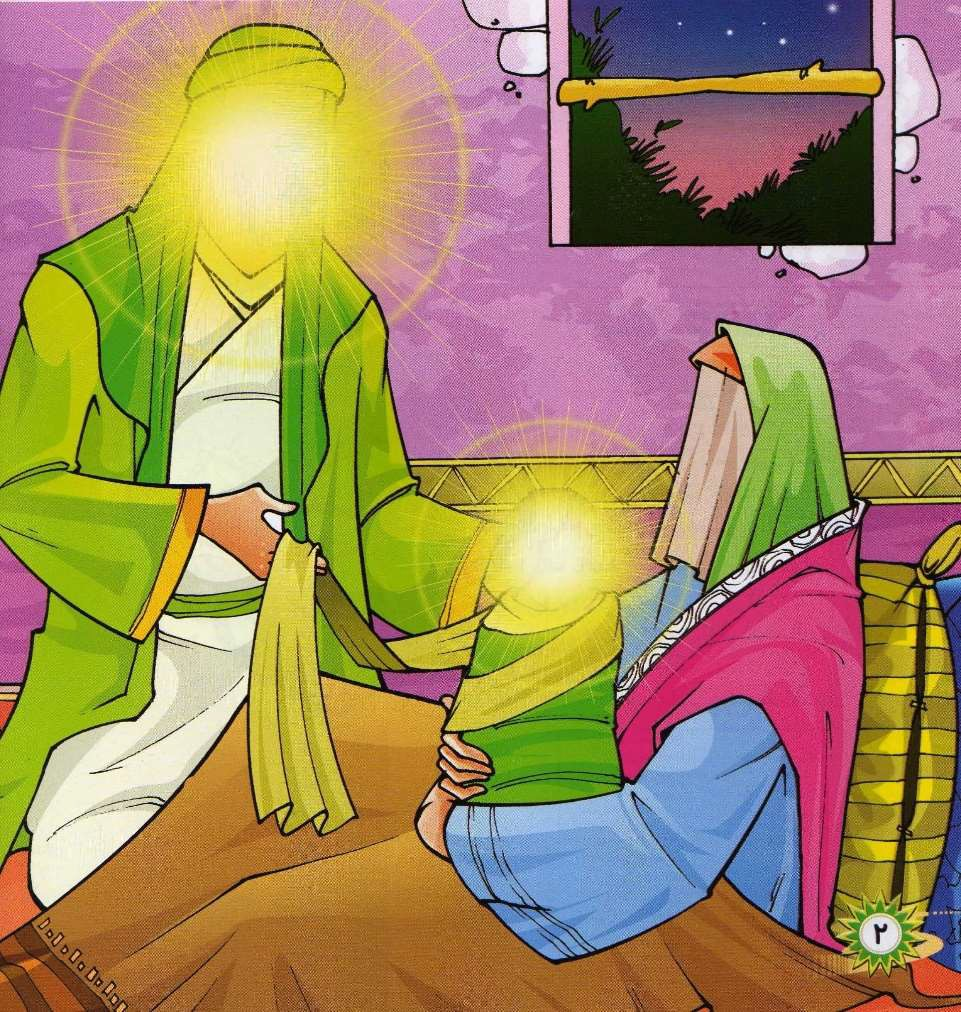
\includegraphics[width=6.3in,height=4.20208in]{media/image4.jpeg}

Selon la théologie musulmane, l'islam est la religion originelle de
l'humanité.VICTOR MOUSSA - STOCK.ADOBE.COM

\subsection{► Que dit la tradition ?}

Selon la théologie musulmane, l'islam est la religion originelle de
l'humanité.~\emph{« Tout homme est né musulman »,}~dit un hadith
attribué
au~\href{https://www.la-croix.com/sacralite-prophete-lislam-2020-11-06-1101123195}{\underline{prophète
Mohammed}}. L'homme est né pour adorer Dieu : certes, il a reçu une
dignité plus haute que les autres créatures, mais celle-ci est
conditionnée à sa soumission au Dieu unique. Plus un homme applique la
loi divine (\emph{charia}), plus il devient humain. Quant au « mécréant
» (\emph{kâfir}), qui refuse de suivre la charia, il se situe en quelque
sorte à un degré inférieur d'humanité.

Cette sévérité envers les non-musulmans s'appuie sur la lecture du texte
coranique qui s'est imposée à partir du IX\textsuperscript{e}~siècle,
lors de la transformation de l'islam en un empire soucieux de se
légitimer. Confortée par des hadiths rédigés à cette époque, elle
dépeint une vérité unique et non négociable. Elle insiste sur les
versets du Coran particulièrement virulents envers les polythéistes,
païens ou idolâtres, qualifiés d'\emph{« associateurs
»}~(\emph{mouchrikoun}) car ils « associent » à Dieu d'autres divinités.

Quant aux athées,~\emph{« ils appartiennent, selon la théologie
musulmane, à une catégorie de mécréance encore inférieure aux
polythéistes, aux juifs et aux chrétiens »,~}explique l'islamologue
Abdessamad Belhaj, chercheur au Centre interdisciplinaire d'études de
l'islam dans le monde contemporain de l'Université catholique de
Louvain. Même si des institutions comme le Haut Conseil des oulémas du
Maroc ou la Maison de la fatwa en Égypte considèrent que les apostats ne
peuvent plus être condamnés à mort, cette peine reste appliquée dans une
dizaine de pays, comme l'Afghanistan ou
la~\href{https://www.la-croix.com/Monde/Afrique/prisons-Mauritanie-calvaire-dun-apostat-2019-09-30-1201051050}{\underline{Mauritanie}}.

\subsection{ Pourquoi juifs et chrétiens bénéficient-ils d'un statut
spécifique ?}

Selon la tradition musulmane, chrétiens et juifs font l'objet d'un
traitement différent des autres non-musulmans : ils bénéficient dans le
droit islamique d'une protection juridique particulière (\emph{dhimma})
toutefois accompagnée d'injonctions humiliantes, comme l'interdiction de
monter à cheval ou de construire des lieux de culte dépassant ceux des
musulmans.
 

\emph{« Le Coran est très ambivalent au sujet des ``gens du Livre''
»,~}rappelle
l'historien~\href{https://www.la-croix.com/Culture/Livres-et-idees/historiens-decryptent-Coran-avant-lislam-2019-11-27-1201063090}{\underline{Guillaume
Dye}}, professeur à l'Université libre de Bruxelles (1). Selon la
sourate 5, juifs et chrétiens ne doivent pas être pris pour~\emph{«
alliés »~}(5, 51) mais, quelques versets plus loin, on lit qu'ils ne
seront~\emph{« point affligés »~}(5, 69). Les chrétiens se voient
reprocher de nier l'unicité de Dieu mais du respect est exprimé pour les
prêtres et les moines, qui~\emph{« ne s'enflent pas d'orgueil ».}

Selon une théologie dite de la falsification (\emph{tahrif}), les juifs
et les chrétiens ont altéré le message transmis par leurs prophètes
respectifs (Moïse, Jésus), message qui n'était autre que l'islam. Le
Coran, lui, corrige cette déviation en transmettant fidèlement le
message révélé à un ultime prophète, Mohammed. À Médine, celui-ci aurait
signé une~\emph{« Constitution »~}disposant que les juifs, notamment,
pouvaient pratiquer leur religion en sécurité, mais ces relations se
sont rapidement détériorées.

\subsection{► Quelles pistes pour une « théologie du pluralisme » ?}

Les attentats visant des « mécréants » en terrasse à Paris, les
persécutions contre les Yézidis ou les chrétiens en Irak, sont autant de
conséquences d'une lecture littéraliste du Coran encouragée par l'essor
du salafisme saoudien à partir des années 1970. D'autres lectures ont
pourtant existé dès les premiers siècles de l'islam. Contrairement à la
doctrine sunnite traditionnelle, l'exégèse rationaliste a par exemple
conclu très tôt à une~\emph{« égalité entre tous les êtres humains, tous
étant dotés de la même raison les rendant aptes à comprendre la parole
de Dieu »,~}rappelle l'islamologue Pierre Lory, directeur d'études à
l'École pratique des hautes études (EPHE).

Pour Abdessamad Belhaj, tout l'enjeu est aujourd'hui de refonder le
rapport à l'altérité sur la base de l'éthique, et de\emph{~« mettre
l'homme au cœur de la théologie »}. Pour cela, certaines valeurs
présentes dans l'islam gagneraient à être redécouvertes, comme celles du
soin, du don et du service à l'humanité, longtemps éclipsées selon lui
par l'autorité et la loyauté à la communauté musulmane ou à la tribu.

(1) Il a codirigé avec Mohammad Ali Amir-Moezzi, Le Coran des
historiens, 2019, Éd. du Cerf, 3~408~p., 89~€.

Faudra-t-il sauver les salafistes ?

Le gouvernement français a voulu lancer en octobre 2019 une offensive
contre l'islamisme et les courants radicaux, rapidement relayée par un
emballement médiatique qui a échappé à tout contrôle. Or, l'ennemi
désigné n'a nullement été identifié selon des termes juridiques, pas
plus que ses torts. On lui reproche sa piété rigoureuse, son voile, sa
pratique du jeûne de Ramadan, sa barbe fournie, son refus de toucher les
femmes, ce qui le rapproche dangereusement de n'importe quel fidèle
conservateur.

L'offensive vise donc une manière de concevoir la piété musulmane, et
nullement une qualification criminelle ou une atteinte à l'ordre public.
C'est dire que nous sommes confrontés à un « délit de sale gueule »,
lequel échappe à la tradition juridique républicaine, délit qui est
indiscernable, sans limite, extensible, mais politiquement pratique
auprès d'une opinion chauffée à blanc par les attentats et
l'immigration.

\subsection{Un engagement d'abord religieux}

Si l'islamiste ainsi décrit ressemble évidemment
au~\href{https://www.la-croix.com/Religion/Islam/Quest-salafisme-2018-10-14-1200975866}{\underline{salafiste}},
c'est oublier un peu vite que l'écrasante majorité des~\emph{salafi~}--
ceux qui sont attachés au modèle des « anciens » (les~\emph{salaf}),
c'est-à-dire les compagnons du Prophète -- se veulent quiétistes : leur
mode d'action est la prédication et l'action missionnaire
(la~\emph{da`wa}). Le salafiste souhaite d'abord vivre un islam épuré et
intégriste -- au sens d'intégral -- dans le cadre de sa famille et de sa
communauté.

Ce mouvement est distinct d'un engagement politique, de sorte que les
salafistes sont rarement liés aux Frères musulmans, qui eux forment un
mouvement politique. Si la matrice religieuse et idéologique du
salafisme imprègne les mentalités djihadistes, elle ne se confond pas
avec celles-ci, ni dans la pensée, ni dans les faits. La radicalisation
concerne donc à des degrés différents et sous des formes incomparables
les sympathisants du salafisme et les partisans du djihadisme de Daech.
Les premiers ont un engagement d'abord religieux, tandis que les autres
sont mus à la fois par la volonté de puissance, des facteurs politiques,
sociaux et religieux.

\subsection{L'autodidacte de l'islam présente plus de risques que le
salafiste}

L'hostilité des salafistes envers les courants djihadistes a été prouvée
à de nombreuses reprises par des déclarations publiques et surtout en
fournissant du renseignement de qualité auprès des services de police.
Le meilleur ennemi du terroriste est souvent le~\emph{salafi}, et
l'autodidacte de l'islam présente plus de risques que le salafiste.

En outre, le salafisme n'a pas été désavoué par les représentants du
culte musulman pour la simple raison que ce courant n'est pas une
idéologie : il faudrait donc lui enlever son~\emph{isme}~final et
l'appeler, selon la tradition religieuse, la~\emph{salafiya~}; il s'agit
d'un vieux courant légitime de l'islam, qui a fourni des générations
d'imams et de lettrés attachés au sens littéral du Coran et de la Sunna.

\subsection{Un « écosystème » étroit mais rassurant}

Il est évident que le salafisme représente une alternative culturelle et
sociale au modèle français, modèle égalitaire, inclusif, ouvert (au
moins en théorie). Les quelques salafi que j'ai connus -- des convertis
à 25 ou 30 \% d'entre eux -- vivaient dans un étroit triangle
géographique. Parce qu'ils souhaitent faire les cinq prières à leur
heure, sans les décaler, et ce dans une salle de prière, ils sont
contraints de vivre et de travailler non loin d'une mosquée. Ils passent
ainsi de leur habitation au lieu de travail et à la salle de prière,
lesquels se situent nécessairement dans un « écosystème » étroit mais
rassurant. Ils ne peuvent guère être exigeants sur le plan
professionnel.

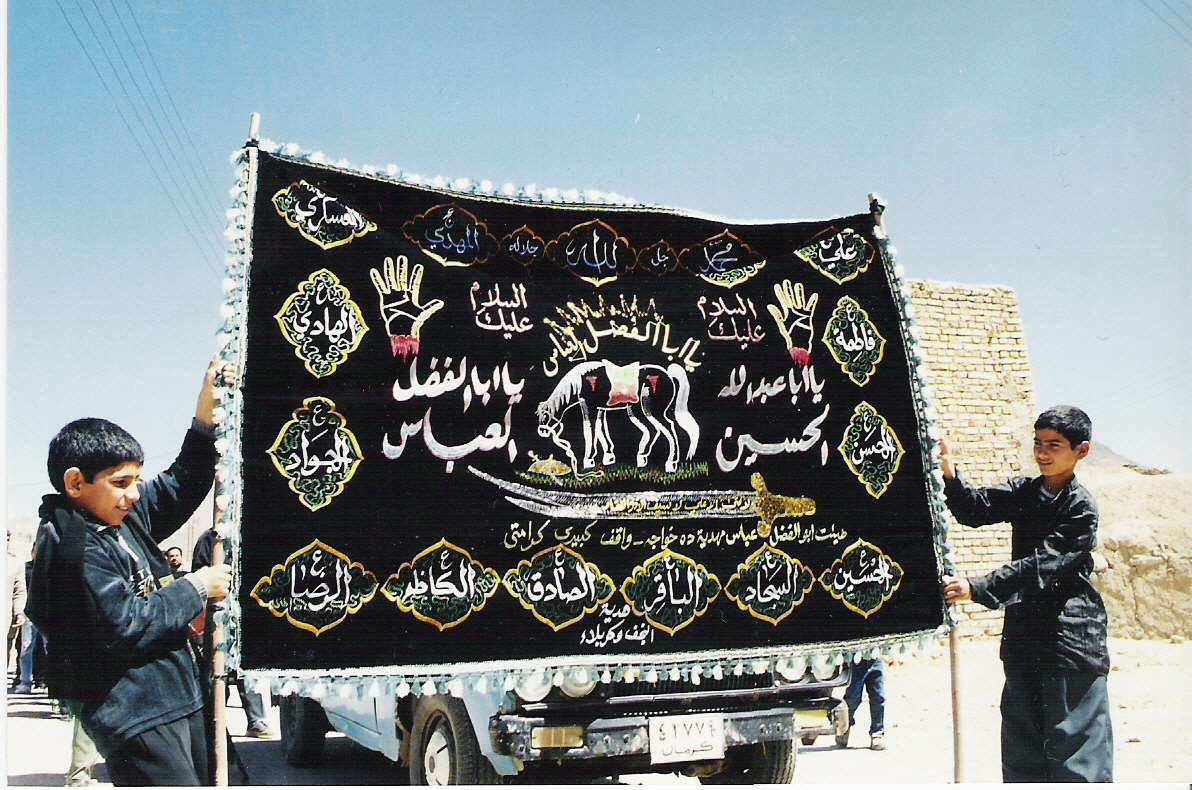
\includegraphics[width=1.97917in,height=1.40972in]{media/image6.jpeg}

\href{https://www.la-croix.com/Religion/Le-Coran-peut-etre-interprete-2021-01-25-1201136852}{Le
Coran peut-il être interprété ?}

Le salafisme, qui représente au moins 40 000 individus, est socialement
dangereux car il impose l'auto-ségrégation, le refus des contacts avec «
ceux qui n'en sont pas ». C'est la raison pour laquelle les spécialistes
des questions de sécurité se refusent à les impliquer dans la lutte
contre le djihadisme. Salafistes et terroristes participeraient à une
même matrice intellectuelle, celle du bien contre le mal, une sorte de
vision sectaire du monde. La différence vient du rapport à la violence :
assumé chez les djihadistes, rejeté chez les salafistes. Leur
fondamentalisme présente l'avantage d'une certaine forme de morale : à
Sartrouville les quartiers salafisés ont vu s'effondrer la toxicomanie
et la délinquance, avec le soutien de la mairie.

\subsection{Confondre l'approche culturelle avec la lutte contre le
terrorisme}

Ces courants ne peuvent être incriminés sur le plan sécuritaire. On
confond donc l'approche culturelle avec la lutte contre le terrorisme. À
moins de changer tout le droit européen, la première doit être menée par
l'éducation, la philosophie, la raison, le débat ; quant à la seconde
elle doit s'appuyer sur le droit et sur des qualifications pénales, et
non sur de vagues impressions de « radicalisation », notion qui n'a
toujours pas été appréhendée de façon rigoureuse en termes sociologiques
et psychologiques.

Comme la guerre d'Algérie nous l'enseigne, une telle manière de
concevoir l'action politique va aboutir à l'effet inverse de celui
recherché : le renforcement de la méfiance collective, le repli
communautaire du côté musulman, l'action violente du côté des « anti »,
et, finalement, la fragmentation sociale et l'insécurité.

\subsection{Islam : les fumées de la radicalisation}

Olivier Hanne, médiéviste (université de Poitiers), chercheur en
islamologie, estime qu'il est très difficile de définir le parcours type
d'une personne radicalisée. Le dernier de trois articles consacrés à
l'islam en France. 
 

Qui parle d'islam aujourd'hui pense aussitôt à la radicalisation. En
2015, on estimait entre 8 000 et 10 000 le nombre de Français
radicalisés. Leurs profils sont si variés qu'il est difficile de donner
des catégories fixes : les mineurs représentent 25 \% des cas, les
femmes 27 \%, les personnes signalées sont plutôt jeunes (entre 16 et 30
ans), leur niveau scolaire est généralement faible, même si l'on
rencontre des diplômés.

La plupart travaillent. Internet représente pour tous ces individus un
passage obligé, même s'il se concrétise différemment : terrain initial
de la radicalisation, facteur de renforcement ou vecteur unique de
l'expression radicale, le partage des contenus djihadistes sur Internet
n'a pas du tout la même fonction chez une adolescente connectée, un
salafiste convaincu et un combattant expérimenté déjà parti en Syrie.

\subsection{Les autorités font feu de tout bois}

De toute évidence, l'attraction pour la radicalité religieuse n'est pas
nécessairement liée à un phénomène de rupture sociale. Les failles de la
société contemporaine (éclatement des familles, déclin des autorités et
des idéologies, chômage, ghettoïsation) créent un terreau facilitateur,
mais nullement déterminant. La frustration individuelle alimente le
recours à des convictions extrêmes, voire le passage à l'acte
terroriste, mais n'est qu'un facteur parmi tant d'autres.

Les autorités font feu de tout bois pour tenter de faire face à une
radicalisation multiforme. En avril 2015, le premier ministre français,
Manuel Valls, annonçait l'ouverture d'une dizaine de centres de
prévention de la radicalisation, dont la plupart furent un échec. Des
sites Internet officiels sont créés et proposent des fiches techniques
contre la radicalisation et le terrorisme, dont le contenu est souvent
simple, voire binaire. Ainsi sur le site
français~\emph{stop-djihadisme.gouv.fr}, un bandeau intitulé «
Radicalisation djihadiste, les premiers signes qui peuvent alerter »
énonce pêle-mêle : « ils se méfient des anciens amis qu'ils considèrent
maintenant comme des impurs » ; « ils changent brutalement leurs
habitudes alimentaires » ; « ils arrêtent d'écouter de la musique car
elle les détourne de leur mission » ; « ils ne regardent plus la
télévision et ne vont plus au cinéma ». Autant de signes extérieurs qui
se rapprochent de l'adolescente anorexique\ldots{} L'efficacité de ces
dispositifs a d'ailleurs été très contestée dès 2015.

\subsection{L'État, tenté d'être omniprésent}

Toute l'entreprise de déradicalisation définit en creux le modèle
positif occidental : monde de loisirs, de consommation, d'épanouissement
personnel et professionnel. Le vocabulaire de la radicalisation masque
le rejet de ce modèle culturel. Et les pouvoirs publics d'hésiter à
appeler leur objectif par son vrai nom : le reconditionnement mental.

Le danger de la déradicalisation se situe dans l'élargissement des
intrusions de l'État : en voulant réinsérer, l'État pénètre dans
l'intimité des individus afin de redéfinir le religieux et lui redonner
une place acceptable. Or, l'État a-t-il compétence pour définir ce
qu'est l'islam, le « bon » islam ? Ne sachant cerner la menace, l'État
est tenté d'être omniprésent, sans en avoir la capacité légale. La
déradicalisation pourrait relever de la posture intellectuelle.

Le problème vient sans doute des hésitations du vocabulaire. Car,
après-tout, qu'est-ce que la radicalisation ? Au
XIX\textsuperscript{e}~le mot anglais~\emph{radical}~était employé pour
désigner les partis politiques britanniques exigeant une réforme
démocratique libérale. Transféré tel quel en France, on l'appliqua aux
partis de gauche, laïques et libéraux qui voulaient réformer la société.

\subsection{Réactions épidermiques}

Le verbe « radicaliser » fut employé régulièrement dans les années
1960-1970 dans une acception politique avec l'idée de « devenir plus
intransigeant, se durcir » ou « plus extrême ». Le premier sens était
donc politique et pas nécessairement négatif. Se déradicaliser était un
synonyme pour « se compromettre ». Appliqué à l'islamisme, le verbe
impose une redéfinition complète des termes : à partir de quand
juge-t-on l'islam intransigeant ou extrême ? par rapport à quelle norme
? à quelle moyenne ?

Les réactions épidermiques qui ont suivi le meurtre de l'enseignant de
Conflans-Sainte-Honorine en octobre 2020 sont tristement révélatrices :
les imams doivent s'exprimer ! les musulmans doivent désavouer le
terrorisme et faire allégeance à la France ! Mais quand ils le font,
c'est encore insuffisant, déloyal et mensonger. Le gouvernement proposa
même qu'ils prient pour la République au cours de la prière collective
du vendredi. Nos références sur la question religieuse restent
tragiquement celles de la Révolution française : comme il y eut les «
prêtres jureurs », adhérant à la loi, contre les « prêtres réfractaires
», obstinés dans leur obéissance à Rome, de la même façon il nous faut
des « imams jureurs », intimement républicains. L'État se retrouve donc
juge des reins et des cœurs.

%\bibliography{Theo}
%\bibliographystyle{siam}
\printbibliography

\listoftheorems[ignoreall,show={Def}]
%Les courants contemporains de l’islam Glossaire général

\mn{Vérifier les termes}

bid‘a : innovation ; pratique « déviante ».

da‘wa : invitation ; prédication – appel à la conversion (dans les deux sens).

fasiq : pécheur ; mauvais musulman.

fiqh : compréhension ; corpus du droit musulman.

fitna: discorde, querelle ; conflit interne au monde musulman.

hadith : récit d’un dire ou faire du Prophète, rapporté par ses compagnons.

hajj : pèlerinage annuel à La Mecque.

hijra (héjire) : « exode » - départ de Mahomet pour Médine (622).

‘ibadat : culte ; partie du droit traitant du culte.

ijma‘ : consensus ; consensus des ulama sur un point de droit.

ijtihad : effort ; effort d’interprétation du Coran.

imam : chef suprême de la communauté musulmane ; successeur du Prophète, utilisé communément par les chiites pour Ali et ses descendants.

islah : réforme.

isnad : chaîne ; chaîne de transmission des hadiths.

jihad : lutte ; soit intérieure, contre ses propres faiblesses ; soit extérieure, contre les ennemis de la communauté musulmane.

ka‘aba : monument cubique noir situé au centre de la grande mosquée de La Mecque ; selon les musulmans, désigne l’emplacement du premier autel élevé par Abraham pour le Dieu unique. Point vers lequel se dirigent les musulmans pour prier.

kafir : infidèle, mécréant

khalifa (calife) : successeur, représentant ; successeur du Prophète et chef de la communauté musulmane (sunnisme).

madrasa : école ; lieu où est assuré la transmission du savoir religieux.

mihrab : niche indiquant la direction de La Mecque dans une mosquée.
 
mu‘amalat : relations ; partie du droit traitant des relations humaines.

qibla : orientation de la prière rituelle (salat), correspondant à la direction de La Mecque.

qiyas : raisonnement par analogie (domaine du droit)

salat : prière rituelle.

seyyed : prince, chef ; descendant du Prophète par Hossein ou Hassan, fils d’Ali.

shari‘a : sentier, voie ; loi divine.

sheykh (cheykh) : vieil homme ; chef d’une tribu ; chef religieux ; personne à la tête d’une congrégation soufie, ayant la capacité de guider ses disciples.

shirk : associationnisme : fait d’adorer d’autres êtres en dehors de Dieu.

shura : principe de consultation soufi : mystique musulman sourate : chapitre du Coran
sunna : coutume ; pratiques du Prophète et de la première communauté musulmane, faisant autorité pour guider le mode de vie des croyants et déterminer la loi religieuse.

tafsir : commentaire du Coran.

tajdid : renouveau (=>mujaddidi : qui renouvelle)

taqlid : imitation ; imitation stérile des anciens (par opposition à l’ijtihad).

tariqa : voie : confrérie soufie.

tawhid : unicité (divine). Dogme fondamental de l’islam.

ulama (oulémas) : terme collectif pour désigner les lettrés musulmans.

umma : peuple ou communauté ; communauté islamique dans son ensemble.

waqf : bien immobilier ou foncier dit « de-main-morte », dépendant des institutions religieuses.

zakat : aumône rituelle, obligatoire pour les croyants.

%\listoftheorems


\end{document}